\documentclass[12pt,twoside]{book}

%Para identar as sub-fases do cap�tulo de 'Metodologia de Trabalho':
\makeatletter
\newenvironment{fase}
               {\list{}{\listparindent 2em%
                        \itemindent    0em%                     
% Se quiser identar a margem direita tamb�m, colocar aqui:  \rightmargin   \leftmargin
                        \parsep        \z@ \@plus\p@}%
                \item[]}
               {\endlist}
\makeatother


\usepackage[brazil]{babel}
\usepackage{multirow}
\usepackage{colortbl}
\usepackage{xcolor}

%para figura composta
\usepackage{subfigure}



%%% bibliografia
\usepackage{natbib}

\usepackage{setspace}

\usepackage{array}

%%% referencias com p�gina \vref
\usepackage[brazil]{varioref}

%%% identa primeiro par�grafo
\usepackage{indentfirst}

%%% definir t�tulos de se��o
\usepackage[sf,sl,outermarks]{titlesec}
%\usepackage{placeins}

%%% lista de abreviaturas
\usepackage{acronym}

%%% boxes
\usepackage{fancybox}

\usepackage[pdftex]{hyperref}

%%% somente na vers�o PDF

%%% Para inclus�o de gr�ficos
\usepackage[pdftex]{graphicx}

%%% dimens�es do documento
\usepackage[pdftex]{geometry}
  \geometry{a4paper,left=3cm,right=2cm,top=2.0cm,bottom=2.0cm,twoside}

%%% cria links no arquivo .pdf
%%% comentar as linhas na vers�o para impressao
\usepackage{hyperref}

%Incluindo algoritmos no texto:
\usepackage[chapter]{algorithm}
\usepackage{algorithmic}

%%% propriedades do arquivo .pdf
\hypersetup{
    pdftitle = {},
    pdfsubject = {},
    pdfkeywords = {},
    pdfauthor = {}
    }



%\hypersetup{colorlinks=true,linkcolor=blue,citecolor=blue}
\hypersetup{colorlinks=true,linkcolor=black,citecolor=black}

%%fonte
\usepackage{ae}
\usepackage[T1]{fontenc}


\DeclareFixedFont{\numberfont}{T1}{phv}{bx}{n}{2cm}

%%% redefine o formato do t�tulo
\titleformat{\chapter}[display]
  {\normalfont\Large\sffamily
  }
  {%\titlerule[3pt]%
   \filright
   \rule[32pt]{.7\linewidth}{4pt}
   \hspace{-11pt}
   \shadowbox{
   \begin{minipage}{.18\linewidth}
     \begin{center}
       \textsc{\Large\chaptertitlename}\\
       \vspace{1ex}
       {\numberfont\color[gray]{0.5} \thechapter}\\
       \vspace{1ex}
     \end{center}
   \end{minipage}}
  }
  {0pt}
  {\filcenter
   \Huge
   }
  [\hfill\rule{.8\textwidth}{0.5pt}]


%%% macro para destacar a(s) primeira(s) letra do texto
%%% � necess�rio ter a fonte courier instalada
%
%  um texto do tipo:
%
%  \begin{document}
%    \versal{IN} THE beginning God created the heaven and the earth.  Now the
%    earth was unformed and void, and darkness was upon the face of the
%    deep; and the spirit of God hovered over the face of the waters.
%  \end{document}
%
%  ir� produzir algo como:
%
%  I I\  I THE beginning God  created the heaven and  the earth.
%  I I \ I Now the earth was unformed and void, and darkness was
%  I I  \I upon the face of the deep; and the spirit of God hov-
%  ered over the face of the waters.

\font\largefont= pzcmi scaled 6500

\newcommand{\versal}[1]{{\noindent
    \setbox0\hbox{\largefont #1 }%
    \count0=\ht0                   % height of versal
    \count1=\baselineskip          % baselineskip
    \divide\count0 by \count1      % versal height/baselineskip
    \dimen1 = \count0\baselineskip % distance to drop versal
    \advance\count0 by 1\relax     % no of indented lines
    \dimen0=\wd0                   % width of versal
    \global\hangindent\dimen0      % set indentation distance
    \global\hangafter-\count0      % set no of indented lines
    \hskip-\dimen0\setbox0\hbox to\dimen0{\raise-\dimen1\box0\hss}%
    \dp0=0in\ht0=0in\box0}}

\definecolor{violet}{rgb}{0.8,0.2,0.5}
\newcommand{\violet}[1]{\textcolor{violet}{#1}}
\newcommand{\PosProcessamento}{P�s-Processamento }



\begin{document}

\frontmatter{}

\pagestyle{empty}
\pagenumbering{roman}

%%% insere a capa
%%% edite os campos para t�tulo, data, orientador e nome

\begin{titlepage}

\setlength{\parindent}{0pt}
\sffamily

\vspace*{3cm}

\rule{.75\linewidth}{.3mm}\par
\Large \textbf{Solu��o interativa para EaD em TV digital} \par
\large \textbf{Parte 1 - Entendendo o problema} \par
\rule{.75\linewidth}{.3mm}\par

\vspace*{2cm}
\textbf{Alunos:} \par
Francisco Belda\\
Marco Aur�lio Graciotto Silva \\
Rodrigo Eduardo Botelho Franciso \\


\vspace*{2cm}
\textbf{Disciplina:} \\
SCE 5812 - Intera��o Usu�rio-Computador \par
\textbf{Prof�.:} \\
Dr�. Maria da Gra�a Campos Pimentel



\vspace{3cm}
USP - S�o Carlos \\
Outubro/2007

\vfill

\cleardoublepage
\end{titlepage}



\onehalfspacing %Para um espa�amento de 1,5

%%% insere o resumo
%%% edite para colocar o seu resumo

\thispagestyle{empty}
\chapter*{Dedicat�ria}
\thispagestyle{empty}

%\addcontentsline{toc}{chapter}{Dedicat�ria}

\vspace*{15cm}
%\begin{titlepage}

\begin{flushright}

\textit{\textit{Aos meus amados pais,\\
				Lindinalva e Conrado.\\
				\vspace{2em}}}

\end{flushright}

\cleardoublepage

\thispagestyle{empty}
\chapter*{\centering{Agradecimentos}}

\rule{\linewidth}{2pt} \vspace{0.2cm}

A Deus, por iluminar o meu caminho.

� minha m�e, por seu amor incondicional, por ter me ensinado a batalhar pelos sonhos e a ser forte perante as dificuldades.  

� minha irm� pela amizade, pelo imenso amor que tem por mim, pelo companheirismo e por me apoiar sempre.

Aos meus irm�os, pelo carinho.

� minha orientadora, professora Dra. Renata Pontin de Mattos Fortes, pelos ensinamentos, pelas partilhas e, sobretudo, pela amizade e pela confian�a que depositou em mim como sua primeira aluna de doutorado. 

� professora Dra. Rosely Sanches pelas in�meras e valiosas contribui��es durante o desenvolvimento do trabalho, pelo carinho e por transmitir uma energia t�o positiva.

Ao professor Dr. Jos� Carlos Maldonado, pelas excelentes sugest�es e cr�ticas em rela��o ao trabalho, pela disponibilidade em colaborar e pela amizade.  

Aos meus familiares que sempre me incentivaram e apoiaram.  

Aos v�rios amigos e colegas, pessoas muito especiais, com as quais convivi nesse per�odo. Aprendi muito com voc�s! Obrigada por terem ajudado a renovar a esperan�a nos momentos dif�ceis e por terem compartilhado os momentos alegres. 

A todos que fizeram e fazem parte do grupo de pesquisa, pela amizade, pelas discuss�es e trocas de experi�ncias t�o enriquecedoras. Em especial ao Andr� Pimenta Freire, pelas expressivas contribui��es. 

Aos professores, funcion�rios e estudantes do Departamento de Computa��o e Estat�stica da Universidade Federal de Mato Grosso do Sul, por terem me recebido com tanto carinho.

A todos aqueles que participaram dos estudos de caso realizados, pelas importantes contribui��es.

Ao ICMC-USP pela oportunidade e � CAPES pelo aux�lio financeiro.



\cleardoublepage

%{\huge{\textbf{Resumo}}}

%\hspace{-0.5cm}\rule{\linewidth}{2pt}

%\vspace{3cm}

%\chapter*{\centering{Resumo}}

%\ renata -- Debora, acho que o resumo est� muito sucinto, assim eu dei algumas sugestoes de melhor contextualizar.... inclui as linhas iniciais para falar de processos pois a definicao de processos nem sempre � obvia para os leitores, dai achei melhor dizer que os processos sao os relacionados com a engenharia de software.. uma definicao de processo que acho bem popular � a da wikipeadia: Na ci�ncia da computa��o, processo pode ter v�rios significados:  * Na Engenharia de Software, processo � um conjunto de passos parcialmente ordenados, cujo objetivo � atingir uma meta: entregar um produto de software de maneira eficiente, previs�vel e que atinja as necessidades de neg�cio. Geralmente inclui an�lise de requisitos, programa��o, testes, entre outras tarefas.  Ver tamb�m: processos da ger�ncia de projetos.  * Em Sistemas Operacionais, processo � um m�dulo execut�vel �nico, que corre concorrentemente com outros m�dulos execut�veis. Por exemplo, em um ambiente multi-tarefa (como o Unix) que suporta processos, um processador de texto, um navegador e um sistema de banco de dados s�o processos separados que podem rodar concomitantemente.  ****** Debora, tambem achei que  voce foi muito resumida com relacao a TUDO que voce fez... os levantamentos, e estudos de caso, mas, voce acha que deve ser mesmo bem conciso o resumo?? Ah, porque eu nao sei se os leitores sabem sobre design rationale, eu coloquei um inicio sobre isso ta?

O volume crescente de projetos de pesquisa que envolvem software motiva a realiza��o de an�lises sobre os processos utilizados no desenvolvimento desses projetos, considerando-se as atividades cumpridas, os resultados obtidos e a aplica��o de recursos. Na �rea de Engenharia de Software, processos t�m sido propostos nos �ltimos anos com o objetivo de contribuir para o desenvolvimento de projetos de pesquisa que envolvem software.
Busca-se, de forma geral, auxiliar o gerenciamento dos diversos artefatos que podem ser gerados, por exemplo, modelos, c�digo fonte, relat�rios t�cnicos e artigos cient�ficos. As solu��es apresentadas na literatura come�aram a ser propostas recentemente e, portanto, os estudos realizados nessa �rea apresentam-se em est�gio bastante inicial. %Observa-se que as solu��es cobrem parcialmente um conjunto de requisitos referentes a processos para desenvolvimento de projetos de pesquisas. 
Dessa forma, o objetivo deste trabalho foi definir um processo para o desenvolvimento de projetos de pesquisa envolvendo software, que esteja de acordo com um conjunto de requisitos identificado e que possa contribuir para a evolu��o desses projetos. Para refor�ar a continuidade dos projetos, foi estudada a abordagem de {\it design rationale}, com o objetivo de oferecer meios para que as decis�es de projeto sejam capturadas e registradas em fases espec�ficas do desenvolvimento. O processo de documenta��o foi enfatizado, ou seja, foi investigado como a abordagem de {\it design rationale} poderia ser utilizada para melhorar a documenta��o dos projetos de pesquisa. Como um resultado obtido, um modelo para representa��o de {\it design rationale} foi definido, implementado em uma ferramenta CASE e avaliado em um experimento.

%\anterior, da debora:
%Processos t�m sido propostos nos �ltimos anos com o objetivo de contribuir para o desenvolvimento de projetos de pesquisa que envolvem software. A principal motiva��o � auxiliar o gerenciamento dos diversos artefatos que podem ser gerados, por exemplo, modelos, c�digo fonte, relat�rios t�cnicos e artigos cient�ficos. As solu��es apresentadas na literatura come�aram a ser propostas recentemente e, dessa forma, os estudos realizados nessa �rea apresentam-se em est�gio bastante inicial. Com isso, p�de ser observado que as solu��es cobrem parcialmente um conjunto de requisitos referentes a processos para desenvolvimento de projetos de pesquisas que foi identificado. O objetivo deste trabalho foi, portanto, definir um processo para desenvolvimento de projetos de pesquisa envolvendo software que possa contribuir para a evolu��o desses projetos. O processo de documenta��o foi enfatizado, ou seja, foi investigado como a abordagem de {\it design rationale} poderia ser utilizada para melhorar a documenta��o dos projetos de pesquisa. Como resultado, foi obtido um modelo para representa��o de {\it design rationale}, que foi implementado em uma ferramenta CASE e avaliado em um experimento.   
 
 %l�m disso, observou-se, a partir de relaos apresentados na literatura, que muitos pesquisadores t�m dificuldades em dar continuidade aos projetos de pesquisa, devido a fraca motiva��o para a atividade de documenta��o. Assim, 
\cleardoublepage

\chapter*{Abstract}
\thispagestyle{empty}

% \addcontentsline{toc}{section}{Abstract}

\versal{T}he task of term extraction in textual domains, which is a subtask of the text pre-processing in Text Mining, can be used for many purposes in knowledge extraction processes. These terms must be carefully extracted since their quality will have a high impact in the results. In this work, the quality of these terms involves both representativity in the specific domain and comprehensibility. Considering this high importance, in this work the effects produced in the comprehensibility and representativity of terms were evaluated when different term simplification techniques are utilized in text collections in Portuguese. The term extraction process follows the methodology presented in this work and the techniques used were radicalization, lematization and substantivation. To support this metodology, a term extraction tool  was developed and is presented as ExtraT. In order to guarantee the quality of the extracted terms, they were evaluated in an objective and subjective way. The subjective evaluations, assisted by domain specialists, analyze the representativity of the terms in related documents, the comprehensibility of the terms with each technique, and the specialist's opinion. The objective evaluations, which are assisted by TaxEM and by Thesagro (National Agricultural Thesaurus), consider the number of extracted terms by each technique and their representativity in the related documents. This objective evaluation of the representativity uses the CTW measure (Context Term Weight) as support. Eight real collections of the agronomy domain were used in the experimental evaluation. As a result, some positive and negative characteristics of each techniques were pointed out, showing that the best technique selection for this domain depends on the main pre-established goal, which can involve obtaining better comprehensibility terms for the user or reducing the quantity of extracted terms.

\cleardoublepage

\setcounter{page}{1}


\addcontentsline{toc}{section}{Sum�rio}
\tableofcontents


\cleardoublepage

%Para colocar lista de Figuras e de Tabelas na mesma p�gina:
%\chapter*{\listfiguretablename{}}


\listoffigures
\addcontentsline{toc}{section}{Lista de Figuras}
\cleardoublepage

\listoftables
\addcontentsline{toc}{section}{Lista de Tabelas}
\cleardoublepage

\listofalgorithms
\addcontentsline{toc}{section}{Lista de Algoritmos}
\cleardoublepage

%\chapter*{Lista de Abreviaturas}

\addcontentsline{toc}{chapter}{Lista de Abreviaturas}

\begin{acronym}[IESystem~]
	
	\acro{API}{\textit{Application Programming Interface}}
	\acro{DF}{\textit{Document Frequency}}
	\acro{EMBRAPA}{Empresa Brasileira de Pesquisa Agropecu�ria}
	\acro{ICMC}{Instituto de Ci�ncias Matem�ticas e de Computa��o}
	\acro{LABIC}{Laborat�rio de Intelig�ncia Computacional}
	\acro{MT}{Minera��o de Textos}
	\acro{NILC}{N�cleo Interinstitucional de Ling��stica Computacional}
	\acro{NSP}{\textit{Ngram Statistics Package}}
	\acro{PreText}{Ferramenta para Pr�-Processamento de Textos}
	\acro{Thesagro}{\textit{Thesaurus} Nacional Agr�cola}
	\acro{TopTax}{Metodologia de extra��o de taxonomias de t�picos}
	
\end{acronym}
%\cleardoublepage

%%% inserir resumo
%%{\huge{\textbf{Resumo}}}

%\hspace{-0.5cm}\rule{\linewidth}{2pt}

%\vspace{3cm}

%\chapter*{\centering{Resumo}}

%\ renata -- Debora, acho que o resumo est� muito sucinto, assim eu dei algumas sugestoes de melhor contextualizar.... inclui as linhas iniciais para falar de processos pois a definicao de processos nem sempre � obvia para os leitores, dai achei melhor dizer que os processos sao os relacionados com a engenharia de software.. uma definicao de processo que acho bem popular � a da wikipeadia: Na ci�ncia da computa��o, processo pode ter v�rios significados:  * Na Engenharia de Software, processo � um conjunto de passos parcialmente ordenados, cujo objetivo � atingir uma meta: entregar um produto de software de maneira eficiente, previs�vel e que atinja as necessidades de neg�cio. Geralmente inclui an�lise de requisitos, programa��o, testes, entre outras tarefas.  Ver tamb�m: processos da ger�ncia de projetos.  * Em Sistemas Operacionais, processo � um m�dulo execut�vel �nico, que corre concorrentemente com outros m�dulos execut�veis. Por exemplo, em um ambiente multi-tarefa (como o Unix) que suporta processos, um processador de texto, um navegador e um sistema de banco de dados s�o processos separados que podem rodar concomitantemente.  ****** Debora, tambem achei que  voce foi muito resumida com relacao a TUDO que voce fez... os levantamentos, e estudos de caso, mas, voce acha que deve ser mesmo bem conciso o resumo?? Ah, porque eu nao sei se os leitores sabem sobre design rationale, eu coloquei um inicio sobre isso ta?

O volume crescente de projetos de pesquisa que envolvem software motiva a realiza��o de an�lises sobre os processos utilizados no desenvolvimento desses projetos, considerando-se as atividades cumpridas, os resultados obtidos e a aplica��o de recursos. Na �rea de Engenharia de Software, processos t�m sido propostos nos �ltimos anos com o objetivo de contribuir para o desenvolvimento de projetos de pesquisa que envolvem software.
Busca-se, de forma geral, auxiliar o gerenciamento dos diversos artefatos que podem ser gerados, por exemplo, modelos, c�digo fonte, relat�rios t�cnicos e artigos cient�ficos. As solu��es apresentadas na literatura come�aram a ser propostas recentemente e, portanto, os estudos realizados nessa �rea apresentam-se em est�gio bastante inicial. %Observa-se que as solu��es cobrem parcialmente um conjunto de requisitos referentes a processos para desenvolvimento de projetos de pesquisas. 
Dessa forma, o objetivo deste trabalho foi definir um processo para o desenvolvimento de projetos de pesquisa envolvendo software, que esteja de acordo com um conjunto de requisitos identificado e que possa contribuir para a evolu��o desses projetos. Para refor�ar a continuidade dos projetos, foi estudada a abordagem de {\it design rationale}, com o objetivo de oferecer meios para que as decis�es de projeto sejam capturadas e registradas em fases espec�ficas do desenvolvimento. O processo de documenta��o foi enfatizado, ou seja, foi investigado como a abordagem de {\it design rationale} poderia ser utilizada para melhorar a documenta��o dos projetos de pesquisa. Como um resultado obtido, um modelo para representa��o de {\it design rationale} foi definido, implementado em uma ferramenta CASE e avaliado em um experimento.

%\anterior, da debora:
%Processos t�m sido propostos nos �ltimos anos com o objetivo de contribuir para o desenvolvimento de projetos de pesquisa que envolvem software. A principal motiva��o � auxiliar o gerenciamento dos diversos artefatos que podem ser gerados, por exemplo, modelos, c�digo fonte, relat�rios t�cnicos e artigos cient�ficos. As solu��es apresentadas na literatura come�aram a ser propostas recentemente e, dessa forma, os estudos realizados nessa �rea apresentam-se em est�gio bastante inicial. Com isso, p�de ser observado que as solu��es cobrem parcialmente um conjunto de requisitos referentes a processos para desenvolvimento de projetos de pesquisas que foi identificado. O objetivo deste trabalho foi, portanto, definir um processo para desenvolvimento de projetos de pesquisa envolvendo software que possa contribuir para a evolu��o desses projetos. O processo de documenta��o foi enfatizado, ou seja, foi investigado como a abordagem de {\it design rationale} poderia ser utilizada para melhorar a documenta��o dos projetos de pesquisa. Como resultado, foi obtido um modelo para representa��o de {\it design rationale}, que foi implementado em uma ferramenta CASE e avaliado em um experimento.   
 
 %l�m disso, observou-se, a partir de relaos apresentados na literatura, que muitos pesquisadores t�m dificuldades em dar continuidade aos projetos de pesquisa, devido a fraca motiva��o para a atividade de documenta��o. Assim, 
%
%\newpage

%%% corpo do texto

\mainmatter{}
\pagenumbering{arabic}
\pagestyle{plain}
%%% inclua os seu arquivos a partir daqui
%Introdu��o com exemplo de cita��o \cite{Pressman2000}.

A Figura \ref{fig} � um exemplo de inser��o de figura.

\begin{figure}[!ht]
\centering
  
\includegraphics[width=.4\textwidth]{figura.jpg}
  \caption{\label{fig}Exemplo de inser��o de figura.}
\end{figure}


A Tabela \ref{tab} � um exemplo de tabela.

\begin{table}[!hb]
\centering
\label{tab}
\caption{Frequency of Special Characters}
\begin{tabular}{|c|c|l|} \hline
Non-English or Math&Frequency&Comments\\ \hline
\O & 1 in 1,000& For Swedish names\\ \hline
$\pi$ & 1 in 5& Common in math\\ \hline
\$ & 4 in 5 & Used in business\\ \hline
$\Psi^2_1$ & 1 in 40,000& Unexplained usage\\
\hline
\end{tabular}
\end{table}

% T�tulos dos cap�tulos:
%\chapter{Introducao}
Introdu��o com exemplo de cita��o \cite{Pressman2000}.

A Figura \ref{fig} � um exemplo de inser��o de figura.

\begin{figure}[!ht]
\centering
  
\includegraphics[width=.4\textwidth]{figura.jpg}
  \caption{\label{fig}Exemplo de inser��o de figura.}
\end{figure}


A Tabela \ref{tab} � um exemplo de tabela.

\begin{table}[!hb]
\centering
\label{tab}
\caption{Frequency of Special Characters}
\begin{tabular}{|c|c|l|} \hline
Non-English or Math&Frequency&Comments\\ \hline
\O & 1 in 1,000& For Swedish names\\ \hline
$\pi$ & 1 in 5& Common in math\\ \hline
\$ & 4 in 5 & Used in business\\ \hline
$\Psi^2_1$ & 1 in 40,000& Unexplained usage\\
\hline
\end{tabular}
\end{table}
%\input {Introdu��o}
%\versal{I}ntrodu��o


\chapter{Processo de Minera��o de Textos}
\label{pre_processamento}

%	2.1 Considera��es Iniciais
%	2.2 Processo de Minera��o de Textos
%	2.3 Pr�-Processamento de Documentos
%	2.4 Trabalhos Relacionados
% 	2.4.1 TopTax - Topic Taxonomy Environment
% 	2.4.2 Exemplos de Aplica��es da Minera��o de Textos
%	2.5 Considera��es Finais

%%%%%%%%%%%%%%%%%%%%%%%%%%%%%%%%%%%%%%%%%%%%%%%%%%%%%%%%%%%%%%%%%
%	Considera��es Iniciais
%%%%%%%%%%%%%%%%%%%%%%%%%%%%%%%%%%%%%%%%%%%%%%%%%%%%%%%%%%%%%%%%%

\section{Considera��es Iniciais}
O processo de Minera��o de Textos (MT) � utilizado para descobrir padr�es e co\-nhe\-ci\-men\-to �til em um conjunto de dados textuais. As bases textuais utilizadas no processo de Minera��o de Textos s�o cole��es de documentos em linguagem natural, sem formato predefinido para seus conte�dos \citep{AraujoTarapanoff:2006}. Os textos que n�o obedecem a um padr�o de formata��o s�o chamados \textbf{n�o-estruturados}; os que seguem algum padr�o, como textos cient�ficos que s�o divididos em t�picos pr�-definidos e livros divididos em cap�tulos, s�o denominados textos \textbf{semi-estruturados}. Neste trabalho, tratamos os textos representados em uma linguagem de marca��o como \textbf{textos estruturados}.

A Minera��o de Textos foi ins\-pi\-ra\-da na Minera��o de Dados e por vezes considerada uma sub�rea da mesma. A Mi\-ne\-ra\-��o de Dados pode ser definida como a extra��o de conhecimento impl�cito, previamente desconhecido e potencialmente �til, ou a busca por rela��es e padr�es globais existentes em bases de dados \citep{Frawley:1992}. Minera��o de Textos � uma �rea interdisciplinar, relativamente nova, que engloba: processamento de l�ngua natural, mais particularmente a ling��stica computacional; aprendizado de m�quina; recupera��o de informa��o; mi\-ne\-ra\-��o de dados; estat�stica e visualiza��o de informa��o. A MT oferece a possibilidade de se trabalhar com dados textuais n�o estruturados, enquanto a Minera��o de Dados trabalha com dados estruturados.

O foco deste trabalho � a extra��o de termos (atributos, caracter�sticas), atividade desenvolvida na etapa de Pr�-Processamento do processo de Minera��o de Textos, na qual s�o executadas as transforma��es necess�rias para a adequa��o do formato dos textos dispon�veis para a extra��o de conhecimento.

A seguir, s�o descritas as etapas do processo de Minera��o de Textos.

%%%%%%%%%%%%%%%%%%%%%%%%%%%%%%%%%%%%%%%%%%%%%%%%%%%%%%%%%%%%%%%%%
%	Processo de Minera��o de Textos
%%%%%%%%%%%%%%%%%%%%%%%%%%%%%%%%%%%%%%%%%%%%%%%%%%%%%%%%%%%%%%%%%

\section{Etapas do Processo de Minera��o de Textos}

A Minera��o de Textos � dividida em cinco grandes etapas: Identifica��o do Problema, Pr�-Processamento, Extra��o de Padr�es, P�s-Processamento e Utiliza��o do Conhecimento, conforme ilustrado na Figura ~\ref{fig:md}. Este processo pode ser instanciado de acordo com o objetivo pr�-estabelecido. Cada etapa � discutida a seguir, bem como as defini��es e conceitos necess�rios � sua compreens�o.

\begin{figure}[h]
	\centering
		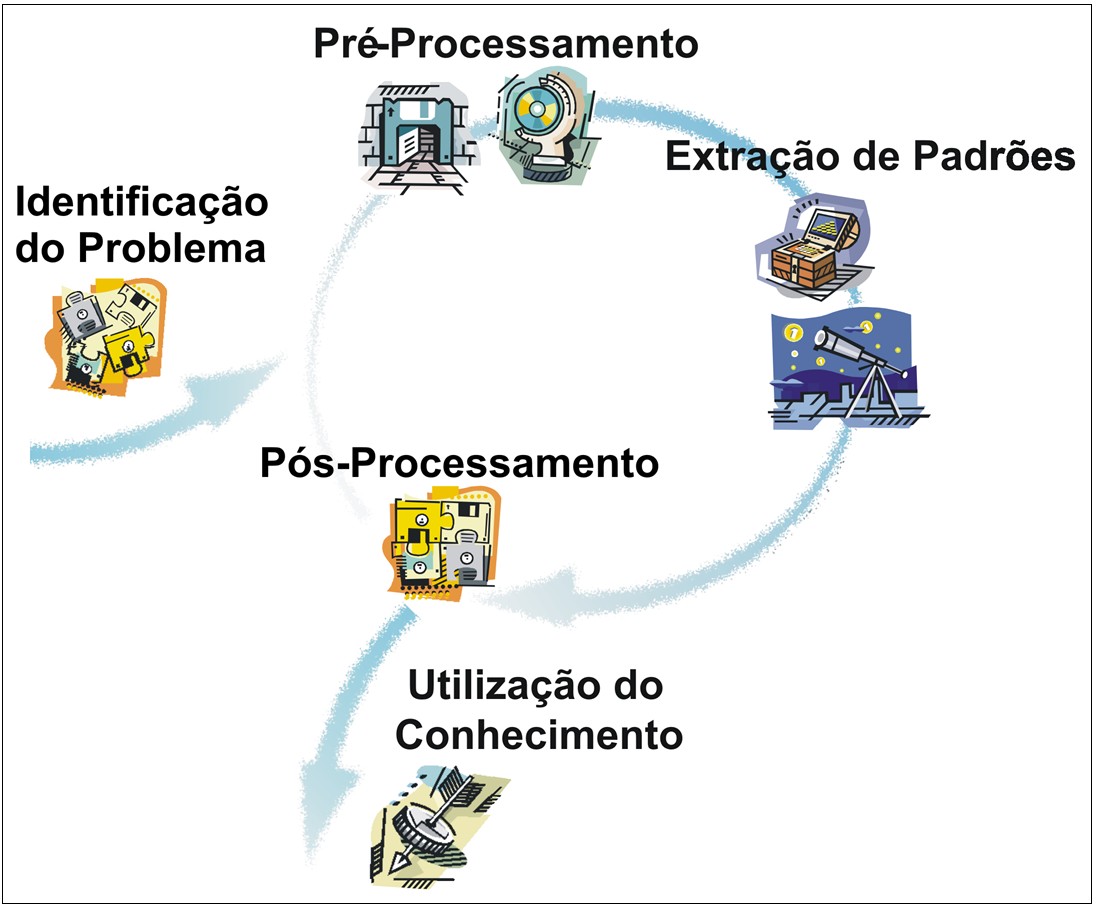
\includegraphics[width=0.75\textwidth]{figuras/md.png}
	\caption{Etapas do processo de Minera��o de Textos \citep{Rezende:2003a}}
	\label{fig:md}
\end{figure}



%----------------------------------------------------------------
%	Identifica��o do Problema
%----------------------------------------------------------------
\subsection{Identifica��o do Problema}

A Identifica��o do Problema � uma etapa muito importante, dado que n�o existe descoberta de conhecimento sem demanda pelo mesmo. Nesta etapa o especialista do dom�nio identifica e delimita o problema, o subdom�nio do problema, a cole��o de textos a ser analisada ou sua fonte de busca, a exist�ncia de algum conhecimento pr�vio de dom�nio que possa ser utilizado na an�lise, o que se espera obter e como os resultados poder�o ser utilizados. � uma etapa que demanda muito esfor�o tanto do especialista do dom�nio quanto do especialista em Minera��o de Textos, pois a mesma fornece subs�dios a todo o processo, permitindo identificar requisitos e poss�veis ferramentas para cada passo.

%----------------------------------------------------------------
%	Pr�-Processamento
%----------------------------------------------------------------
\subsection{Pr�-Processamento}

Na etapa de Pr�-Processamento encontra-se a principal diferen�a entre o processo de Minera��o de Dados e o de Minera��o de Textos. Nos dois casos, o problema resume-se ao fato dos dados n�o estarem sempre em um formato adequado para a Extra��o de Padr�es; � necess�rio adequ�-los para um formato manipul�vel por algoritmos de extra��o de conhecimento, al�m de aplicar-lhes um processo de tratamento, limpeza e, em geral, redu��o do volume de textos, sempre lhes preservando as caracter�sticas necess�rias para que os objetivos do processo de minera��o sejam cumpridos \citep{Batista:2003}.

Nessa etapa, a partir da cole��o de textos, ocorre a prepara��o dos textos para poder extrair os termos importantes da cole��o. Estes termos devem discriminar a cole��o de textos que, por sua vez, � representada na forma matriz atributo-valor, conforme ilustrado na Figura ~\ref{fig:preProc} e detalhado a seguir.

\begin{figure}[h]
    \centering
        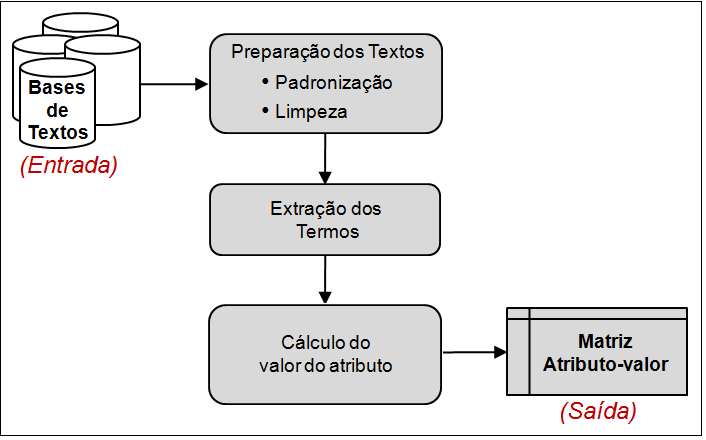
\includegraphics[scale=0.75]{figuras/preProc.png}
    \caption{Etapas do Pr�-Processamento da cole��o de textos - Adaptada de \citet{Moura:2006}}
    \label{fig:preProc}
\end{figure}

Os dados de entrada correspondem � cole��o de documentos de in\-te\-res\-se (\textbf{cole��o de textos}). Esta cole��o pode estar em diferentes formatos, como documentos hipertextos ou formatos \textit{.pdf}. Dependendo de como os documentos foram armazenados ou gerados, h� a necessidade de padronizar as formas em que se encontram. Na \textbf{padroniza��o dos textos}, geralmente, os documentos s�o convertidos para o forma de texto plano sem formata��o.

Em seguida, na \textbf{limpeza dos textos}, elimina-se dos mesmos as {\textit{stopwords}, que s�o aquelas palavras que nada acrescentam � representatividade dos termos ou que sozinhas nada significam, como artigos, pronomes e adv�rbios. Sua defini��o depende dos objetivos estabelecidos e do dom�nio do conhecimento, e seu uso pode ser considerado como uma ``forma de sele��o inicial de termos, pois ajuda a reduzir a dimens�o final do vocabul�rio eliminando termos n�o significativos para a an�lise'' \citep{Moura:2006}. O conjunto de \textit{stopwords} � chamado de \textit{stoplist}. Segundo \citet{ManningRagSchutze:2008}, tal elimina��o reduz significativamente a quantidade de palavras que s�o armazenadas, podendo-se deduzir que a quantidade de palavras que s�o processadas e o tempo gasto para isto tamb�m s�o reduzidos.

%vantagens da utiliza��o de bag of words em RT  N� 205 da Carolina Monard et al p.3
O n�mero de termos que comp�em os textos da cole��o ap�s a remo��o das \textit{stopwords} pode ainda ser muito grande e, em geral, alguns termos se referem ao mesmo conceito. Assim, na \textbf{extra��o dos termos}, faz-se necess�ria a busca por padr�es que simplifiquem as diversas formas de apresenta��o de termos com o mesmo significado essencial. Entre as t�cnicas mais utilizadas para este fim, encontram-se a radicaliza��o, a lematiza��o e a substantiva��o.  Al�m disso, a partir dos termos simplificados, existe a possibilidade de extrair termos compostos e um vocabul�rio controlado, como explicado na Se��o \ref{tecnicasSimplif} do Cap�tulo \ref{extracaoTermos}.

Uma vez extra�dos os termos que representam a cole��o, passa-se � estrutura��o da cole��o textual em uma representa��o que seja manipul�vel por algoritmos utilizados na etapa de Extra��o de Padr�es. A representa��o mais comumente aplicada � cole��o de textos, em tarefas de Mi\-ne\-ra\-��o de Textos com �nfase em m�todos estat�sticos, leva � forma matricial dos documentos \citep{Weiss:2005}. Esta forma matricial dos documentos engloba os termos utilizados e algum \textbf{valor do atributo}, sendo que este valor pode ser, ba\-si\-ca\-men\-te, bin�rio (presen�a ou aus�ncia do termo no texto) ou freq��ncia de ocorr�ncias do termo na cole��o de textos, entre outras \citep{Weiss:2005}. A escolha e c�lculo desse valor do atributo depende do objetivo, e possibilita calcular a re\-pre\-sen\-ta\-ti\-vi\-da\-de de cada termo em seu respectivo documento e/ou na cole��o de textos.%(p�g.29 Moura:2006)

Normalmente, os termos extra�dos de uma cole��o textual s�o tratados como um conjunto desordenado de palavras independentes - conhecido como \textit{bag of words}. A principal limita��o dessa representa��o � considerar apenas a co-ocorr�ncia dos termos. Por exemplo, polissemias (ocorr�ncias de termos cuja grafia � id�ntica ou muito pr�xima), mas cujo significado depende do contexto, s�o tratadas como termos �nicos e si\-n�\-ni\-mos como termos independentes \citep{Dupret:2005}, n�o obtendo, portanto, uma descri��o fiel do conte�do do documento. O efeito negativo das ocorr�ncias de polissemias na cole��o de textos pode ser bastante reduzido quando a cole��o vem de um {\textit{corpus de es\-pe\-ci\-a\-li\-da\-de}, ou seja, de uma cole��o de textos proveniente de um dom�nio de conhecimento espec�fico. %O foco deste trabalho � o tratamento de documentos de um dom�nio espec�fico.

%Baseado no exemplo de \citep{Martins:2003}
A representa��o \textit{bag of words} pode ser estruturada por meio da \textbf{matriz atributo-valor}. Um exemplo dessa representa��o pode ser observado na Tabela \ref{tab:matriz} \citep{Martins:2003}, na qual $d_{i}$ corresponde ao i-�simo documento, $t_{j}$ representa o j-�simo atributo (termo), $a_{ij}$ � o valor do j-�simo atributo no i-�simo documento. O $y_{i}$, que representa a classe do i-�simo documento, n�o est� presente na matriz quando a cole��o de textos � n�o-rotulada.

\begin{table}[h] 
\footnotesize \centering
\begin{tabular}{c|c c c c|c} 
\hline
         & $t_1$    &  $t_2$    & \ldots & $t_M$    & $Y$\\ \hline \hline
  $d_1$  & $a_{11}$ &  $a_{12}$ & \ldots & $a_{1M}$ & $y_{1}$\\
  $d_2$  & $a_{21}$ &  $a_{22}$ & \ldots & $a_{2M}$ & $y_{2}$\\
 $\vdots$& $\vdots$ &  $\vdots$ &$\ddots$& $\vdots$ & $\vdots$ \\
  $d_N$  & $a_{N1}$ &  $a_{N2}$ & \ldots & $a_{NM}$ & $y_{N}$\\ \hline
\end{tabular}
\caption{Padr�o de matriz atributo-valor} \label{tab:matriz}
\end{table}

A matriz atributo-valor � caracteristicamente esparsa e possui alta dimensionalidade, dado que cada palavra presente nos documentos � candidata a a\-tri\-bu\-to da tabela. Entretanto, v�rias dessas palavras n�o est�o presentes em todos os documentos, fazendo com que seus valores internos sejam nulos - ou inexistentes. %N�o diz nada este par�grafo: Ainda, o n�mero de documentos da cole��o e de termos que os descrevem est�o diretamente relacionados � qualidade dos resultados obtidos.

Essa representa��o (matriz atributo-valor) permite o emprego de um grande leque de ferramentas de aprendizado de m�quina, aplicadas ao contexto de Minera��o de Textos.

Ap�s a representa��o matricial dos documentos, pode-se, ainda, diminuir a quantidade de termos a ser trabalhada utilizando abordagens de sele��o de termos, como o m�todo de Luhn, Salton, \textit{Term Variance}. Estes m�todos s�o detalhados no trabalho de \citet{NogueiraDissert:2009}.

Deve-se ressaltar, que esta etapa de Pr�-Processamento pode ser redefinida e ent�o repetida ap�s as pr�ximas etapas, uma vez que a descoberta de alguns padr�es pode levar a estabelecer melhorias a serem empregadas sobre o valor do atributo utilizado na matriz atributo-valor. Por exemplo, o uso de algum fator de pondera��o - estabelecido a partir da presen�a ou aus�ncia de um conjunto de atributos no texto; o uso de algum tipo de taxonomia ap�s a descoberta da mesma; o descarte ou inclus�o de algum voc�bulo ou combina��o deles.


%----------------------------------------------------------------
%	Extra��o de Padr�es
%----------------------------------------------------------------
\subsection{Extra��o de Padr�es}

Na etapa de Extra��o de Padr�es s�o definidas as tarefas a serem realizadas de acordo com o objetivo do processo. Essas tarefas podem ser preditivas ou descritivas.

As \textbf{tarefas preditivas} consistem na generaliza��o de exemplos ou experi�ncias passadas com respostas co\-nhe\-ci\-das.  Essas tarefas utilizam os chamados modelos de aprendizado de m�quina supervisionado, uma vez que as categorias s�o sempre pr�-conhecidas e dispon�veis junto aos dados. Estes modelos podem ser divididos em tarefas de classifica��o, referente ao processo em que o atributo classe tem valor categ�rico, e tarefas de regress�o, na qual busca-se predizer valores de vari�veis que possuem valores cont�nuos.

Por exemplo, a partir da sele��o de uma cole��o de artigos sobre esportes e outros de uma �rea diferente, pode-se inferir um modelo de classifica��o para artigos da �rea de esporte, que � dito uma tarefa de classifica��o. Deve-se observar que a categoria ou classe, nesse caso, � um atributo discreto e que os dados s�o mapeados em um n�mero finito de categorias, no qual cada categoria corresponde a um r�tulo.
J� como exemplo de uma tarefa de regress�o, pode-se considerar a predi��o do ganho ou da perda de produ��o em uma cultura, com base no estudo de diferentes aduba��es no qual a medida de produtividade � um atributo cont�nuo.

Quando apenas parte dos exem\-plos s�o rotulados, podem ser aplicados modelos de aprendizado de m�quina semi-supervisionados, em que a informa��o dos rotulados ajuda a gerar modelos para rotular os dados n�o rotulados, ou aplica-se um m�todo n�o supervisionado para gerar r�tulos e ent�o um classificador para tentar melhorar a rotula��o, repetindo-se o processo enquanto algum crit�rio de avalia��o do mesmo indicar que houve melhora \citep{Matsubara:2003,BrefeldScheffer:2004}.

As \textbf{tarefas descritivas}, por sua vez, consistem na identifica��o de comportamentos intr�nsecos da cole��o de textos, sendo que esses dados s�o exemplos n�o rotulados ou tratados como n�o rotulados. Nestas tarefas, s�o utilizados modelos de aprendizado de m�quina n�o-super\-vi\-siona\-do, e as principais tarefas s�o regras de associa��o, agrupamento (\textit{clustering}), sumariza��o e visualiza��o. 

Nesta etapa de Extra��o de Padr�es, os resultados gen�ricos podem ser validados por m�tricas objetivas ou, ainda, por julgamento subjetivo de especialistas do dom�nio em quest�o, o que pode auxiliar na condu��o da an�lise desses resultados. As valida��es sob esses resultados gen�ricos podem indicar a necessidade de repetir passos do Pr�-Processamento ou mesmo refaz�-lo.     

%----------------------------------------------------------------
%	P�s-Processamento
%----------------------------------------------------------------
\subsection{P�s-Processamento e Utiliza��o do Conhecimento}

O P�s-Processamento � a etapa de valida��o das descobertas efetuadas. � a etapa de avalia��o do conhecimento obtido e a apresenta��o do mesmo, seja por ferramentas de visualiza��o ou simplesmente por tabelas de resultados. A an�lise minuciosa dos resultados obtidos permite que se valide a sua u\-ti\-li\-da\-de e at� mesmo o pr�prio processo, determinando a necessidade de retomar passos anteriores e reestruturando-os se necess�rio. Nesta etapa o especialista do dom�nio e o de Minera��o de Textos devem trabalhar juntos, procurando responder a quest�es como: representatividade do conhecimento obtido;  o que h� de novo nos resultados encontrados;  de que maneira o co\-nhe\-ci\-men\-to do especialista difere do obtido;  valida��o dos resultados obtidos; identifica��o da adequa��o de procedimentos nas etapas anteriores para tentar melhorar os resultados; e de que maneira os resultados obtidos devem ser utilizados.

Na etapa de Utiliza��o do Conhecimento os resultados est�o validados e aptos a serem utilizados. Dessa forma, o conhecimento extra�do pode ser aplicado para apoiar algum processo de tomada de decis�o, conforme objetivo pr�-estabelecido na etapa de Identifica��o do Problema. 



%%%%%%%%%%%%%%%%%%%%%%%%%%%%%%%%%%%%%%%%%%%%%%%%%%%%%%%%%%%%%%%%%
%	Algumas aplica��es da Minera��o de Textos
%%%%%%%%%%%%%%%%%%%%%%%%%%%%%%%%%%%%%%%%%%%%%%%%%%%%%%%%%%%%%%%%%
\section{Algumas aplica��es da Minera��o de Textos}

%arrumar: rever itens, citando exemplo e as respectivas refer�ncias:
Minera��o de Textos tem como principal fun��o identificar, nos mesmos, informa��es singulares, e n�o necessariamente informa��es principais, como � o caso da recupera��o e preserva��o da id�ia central. Todavia, ela pode ser aplicada para diversos fins, como em algumas das aplica��es listadas a seguir.
\begin{itemize}
	\item \textbf{Sumariza��o para documentos n�o estruturados} corresponde a gera��o de sum�rio, um resumo, com o objetivo de transmitir ou comunicar somente o que � importante de uma fonte textual de informa��o \citep{RinoPardo:2003};
%arrumar: verificar o ano do artigo!!!
	\item \textbf{Classifica��o de textos} consiste em classificar novos textos (documentos) pertencentes a um conjunto de documentos pr�-definido em uma ou mais categorias ou classes \citep{Sebastiani:2006}; %consiste em ``induzir um classificador a partir de uma cole��o de documentos de treinamento rotulados, com o objetivo de classificar novos textos (documentos) com uma boa precis�o'' \citep{MartMatsubMon:2003};
	%\item \textbf{Recupera��o de informa��o} visa produzir uma cole��o de documentos relevantes, sem necessariamente condens�-los \citep{RinoPardo:2003};
	\item \textbf{Recupera��o de informa��o} tem como objetivo encontrar documentos que contenham uma determinada informa��o procurada a partir de uma cole��o de textos \citep{ManningEtAl:2008};
%	\item \textbf{Extra��o de informa��o}, que n�o necessariamente tem a condensa��o de informa��o como restri��o fundamental;
	\item \textbf{Extra��o de informa��o} consiste em extrair a partir de documentos alguma informa��o relevante \citep{TurmoEtAl:2006}; %visa extrair a partir de documentos apenas os dados relevantes ao usu�rio; \citep{prudencio:2005};
	\item \textbf{Indexa��o} visa identificar termos convenientes para a recupera��o de informa��o.
	%Tirado Ara�jo J�nior e Tarapanoff 2006
No trabalho de \cite{AraujoTarapanoff:2006} foi feita uma compara��o entre indexa��o manual e indexa��o utilizando uma ferramenta de Minera��o de Textos, por meio da an�lise do �ndice de precis�o de resposta no processo de busca e recupera��o da informa��o.
	\item \textbf{Agrupamento de documentos} almeja descobrir agrupamentos naturais e, ent�o, apresentar as poss�veis classes em uma cole��o de textos \citep{AndFox:2007}.
\end{itemize}



%%%%%%%%%%%%%%%%%%%%%%%%%%%%%%%%%%%%%%%%%%%%%%%%%%%%%%%%%%%%%%%%%
%   Exemplo de instancia��o da Minera��o de Textos: Metodologia TopTax
%%%%%%%%%%%%%%%%%%%%%%%%%%%%%%%%%%%%%%%%%%%%%%%%%%%%%%%%%%%%%%%%%
\section{Exemplo de instancia��o da Minera��o de Textos: Metodologia TopTax}
\label {toptax}

Como exemplo de um processo instanciado de Minera��o de Textos, pode-se citar a metodologia para extra��o de taxonomia de t�picos TopTax (\textit{Topic Taxonomy Environment}) \citep{Moura:2006,ConradoWTI:2008}. Esta metodologia tem como objetivo auxiliar especialistas de um dom�nio espec�fico a organizar e manter a informa��o do mesmo. Tal organiza��o � poss�vel devido � cria��o de uma taxonomia de t�picos. A taxonomia considerada � uma classifica��o hier�rquica de t�picos extra�dos de uma cole��o de textos, na qual os t�picos superiores s�o \textit{pais} dos inferiores, ou seja, os inferiores s�o especializa��es dos t�picos superiores. Al�m disso, a cada n�vel da taxonomia pode-se associar recursos da base textual referentes ao seu dom�nio, facilitando, assim, a organiza��o da informa��o sob essa taxonomia.

Para isto, � necess�rio analisar o conhecimento do dom�nio e construir a hierarquia dos t�picos espec�ficos do dom�nio, isto �, uma taxonomia de t�picos sobre o conhecimento do dom�nio representado pela cole��o de textos, ou os metadados sobre outros tipos de recursos, bem como fornecer crit�rios que possibilitam aos especialistas decidirem sobre o crescimento da cole��o de textos (o limite do aumento da quantidade de textos na taxonomia existente). 

Pode-se haver algumas confus�es em rela��o a defini��o de taxonomia e ontologia. Para a comunidade de Intelig�ncia Artificial, ontologia � ``uma especifica��o de uma conceitua��o'' \citep{Gruber:1995}, isto �, � uma especifica��o expl�cita, com um vocabul�rio formal e regida por axiomas, dos conceitos em um dom�nio e as rela��es entre eles. Considera-se como axiomas as regras pertinentes ao dom�nio em quest�o. Neste sentido, uma taxonomia pode se tornar uma ontologia com a inclus�o de axiomas.

A TopTax, para atingir seus objetivos, conforme mostrado na Figura ~\ref{fig:toptax}, segue as etapas do processo de Minera��o de Textos.

\begin{figure}[ht]
    \centering
        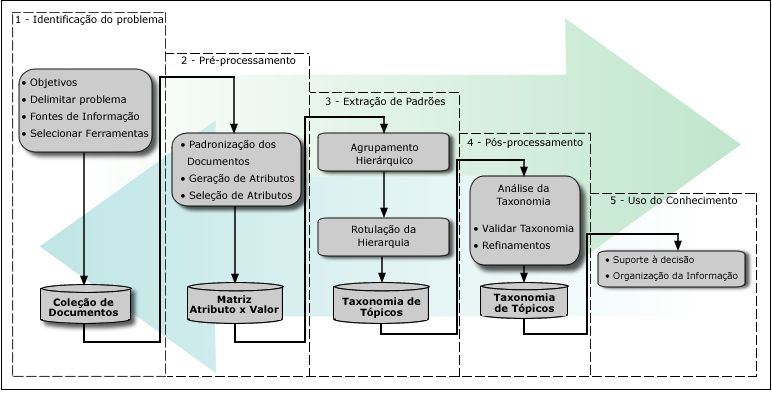
\includegraphics[scale=0.78]{figuras/toptax.png}
    \caption{TopTax - Metodologia de extra��o de taxonomias de t�picos \citep{ConradoWTI:2008}}
    \label{fig:toptax}
\end{figure}

A etapa de Identifica��o do Problema visa delimitar o problema a ser abordado, que no caso � fornecer aux�lio aos especialistas de um dom�nio espec�fico a organizar e manter a informa��o do mesmo. A partir deste problema, pretende-se encontrar uma solu��o para o mesmo, tra�ando o objetivo a ser alcan�ado para que este problema possa ser resolvido, que no caso � a constru��o de uma taxonomia de t�picos do dom�nio em quest�o. Ap�s a defini��o do problema e do objetivo, pode-se, ent�o, com a ajuda de especialistas do dom�nio, recuperar os documentos do mesmo que formar�o a base de textos a ser trabalhada, considerando que esses documentos podem vir de bases e formatos distintos. Al�m disso, nesta etapa s�o selecionadas as ferramentas que auxiliar�o no processo de Minera��o de Textos.

J� na etapa do Pr�-Processamento, os documentos da base de textos obtida s�o preparados para servirem de entrada para as ferramentas que ser�o utilizadas. Esta prepara��o abrange as atividade de limpeza, padroniza��o, extra��o de termos e c�lculo do valor do atributo que ser� utilizado na matriz atributo-valor. Durante a padroniza��o, os documentos que n�o estiverem em formato textual ser�o descartados, mas os que estiverem em fontes de informa��o em formato de figuras e filmes, ser�o considerados seus metadados, caso existam. Na atividade de extra��o de termos que descrevem a base de textos, os termos s�o representados em uma matriz atributo-valor. Mas como a quantidade de termos � muito elevada, utilizam-se t�cnicas que simplifiquem tais termos, o que diminuir� a dimensionalidade dessa matriz, facilitando o seu processamento e, como conseq��ncia, na compreens�o dos termos. Mesmo assim, a dimensionalidade da matriz que representa tais termos pode continuar elevada. Neste caso, a TopTax sugere utilizar m�todos de sele��o de termos, com o objetivo de diminuir a quantidade de termos a ser trabalhada. Como exemplos desses m�todos, pode-se citar os m�todos de Luhn, Salton, e \textit{Term Variance}, que s�o detalhados no trabalho de \citet{NogueiraDissert:2009}.

Em seguida, na etapa de Extra��o de Padr�es, visando a constru��o de uma taxonomia de t�picos, efetua-se o processo de agrupamento hier�rquico de documentos. % para agrupar documentos com conte�dos semelhantes.
Para isso, aplicam-se m�todos de agrupamento hier�rquico, como o \textit{complete linkage}, \textit{average likage} ou \textit{single linkage} \citep{MardiaEtAl:1979}.

Com a hierarquia, os agrupamentos obtidos ret�m t�picos ou sub t�picos aos quais os documentos se referem. Em seguida, conforme descrito em \citet{ConradoWTI:2008}, gera-se os r�tulos para cada grupo encontrado pela obten��o dos termos mais significativos, sendo poss�vel adicionar a cada n� recursos de informa��o de t�picos, como documentos, v�deos e imagens associadas. Por fim, na etapa do P�s-Processamento, esta hierarquia obtida � visualizada e validada para que a mesma possa ser utilizada para dar suporte �s decis�es e organiza��o da informa��o ali contida. Tal visualiza��o e valida��o � apoiada pela ferramenta TaxTools \citep{MarcaciniRezende:2008}.


%%%%%%%%%%%%%%%%%%%%%%%%%%%%%%%%%%%%%%%%%%%%%%%%%%%%%%%%%%%%%%%%%
%	Considera��es Finais
%%%%%%%%%%%%%%%%%%%%%%%%%%%%%%%%%%%%%%%%%%%%%%%%%%%%%%%%%%%%%%%%%

\section{Considera��es Finais}
Neste cap�tulo foram abordados alguns conceitos das etapas do processo de Minera��o de Textos, com �nfase na etapa de Pr�-Processamento, que � o foco deste trabalho. Al�m disso, destacou-se a elevada import�ncia da representa��o dos documentos neste processo.

Foram apresentadas algumas das aplica��es da Minera��o de Textos, bem como um resumo da metodologia TopTax, que � um exemplo de processo instanciado de Minera��o de Textos. Deve-se ressaltar que os passos da metodologia de extra��o de termos apresentada neste trabalho (detalhada no Cap�tulo \ref{abordExtracao}), al�m de outros fins, s�o utilizados na etapa de Pr�-Processamento da TopTax. A metodologia proposta neste trabalho � semi-au\-to\-ma\-ti\-za\-da j� que em determinados momentos ocorre intera��o com especialistas.

No decorrer do desenvolvimento deste trabalho, poder-se-� notar que a escolha de alguns procedimentos serve, tamb�m, para amenizar o pro\-ble\-ma do espa�o de dimens�o muito alta no processo de Minera��o de Textos. Como exemplo desses procedimentos, pode-se citar a limpeza da base de textos, que acarreta na diminui��o do espa�o de armazenamento dos dados trabalhados mantendo a qualidade, visando melhorar o tempo de processamento e o espa�o de armazenamento necess�rio para os dados.

No cap�tulo a seguir � detalhada uma das tarefas do Pr�-Processamento da Minera��o de Textos, que � a Extra��o de Termos.
%\versal{M}inera��o de Textos
%\subsection{Dados, Informa��o e Conhecimento} 

% Ver trabalho do slide 12 da Tati da apresentacao feita pra Solange e Heloisa.

\chapter{Extra��o de Termos para a Minera��o de Textos}
\label{extracaoTermos}
%   3.1 Considera��es Iniciais
%		3.2 Termos Simples e Compostos (tirei)
%   3.3 Identifica��o dos Termos
%		3.4 T�cnicas de simplifica��o de termos
%       3.4.1 Radicaliza��o
%       3.4.2 Lematiza��o
%				3.4.3 Substantiva��o
%   3.5 Extra��o de Termos Simples e Compostos
%		3.6 Vocabul�rio Controlado
%		3.7 Trabalhos Relacionados com a Extra��o de Termos
%   3.7 Ferramentas para Extra��o de termos (onde??)
%   3.8 Considera��es Finais


%%%%%%%%%%%%%%%%%%%%%%%%%%%%%%%%%%%%%%%%%%%%%%%%%%%%%%%%%%%%%%%%%
%   Considera��es Iniciais
%%%%%%%%%%%%%%%%%%%%%%%%%%%%%%%%%%%%%%%%%%%%%%%%%%%%%%%%%%%%%%%%%
\section{Considera��es Iniciais}
O resultado da etapa do \textbf{Pr�-Processamento}, no processo de Minera��o de Textos, � uma re\-pre\-sen\-ta\-��o da cole��o de textos a ser analisada em um formato adequado � etapa de Extra��o de Padr�es. A qualidade dos resultados depende principalmente do trabalho realizado nesta etapa, mais especificamente nas tarefas de sele��o e extra��o dos termos.

%% D�VIDA: como irei tratar qdo o doc que apresenta caracteres inv�lidos ou palavras com erros gramaticais?? Salton (1983) diz pra usar Dictionary lookup.

O \textbf{termo}, tamb�m chamado de \textbf{caracter�stica} ou \textbf{atributo}, pode ser uma palavra simples ou composta. Quando o termo � composto por apenas uma palavra, este � denominado de \textit{unigrama} ou termo simples, e quando � composto por mais de uma palavra, � chamado de \textit{n-grama} (termo composto ou combina��o). Como exemplos de termos simples, pode-se citar: \textit{inteligencia}, \textit{artificial}, \textit{processo}; j� como exemplos de termos compostos, t�m-se: \textit{inteligencia\_artificial} e \textit{processo\_mineracao\_textos}. Deve-se ressaltar que o significado sem�ntico desses termos pode diferenciar quando s�o compostos de uma �nica palavra, como \textit{inteligencia} e quando s�o compostos de mais de uma palavra, como \textit{inteligencia artificial}.

Na etapa de Pr�-Processamento, deve-se extrair termos (simples e/ou compostos) que conceitualmente melhor representam tais cole��es. Isso ajudar� a reduzir o n�mero de termos utilizados, restringindo-os a um conjunto mais representativo da cole��o, a fim de que o processamento desses dados seja uma tarefa computacionalmente mais simples e semanticamente adequada ao dom�nio de conhecimento.

Ressalta-se que alguns pesquisadores da �rea consideram a extra��o de termos como sin�nimo para gera��o de termos, por�m, neste trabalho, estas palavras s�o consideradas como distintas. A gera��o de termos � o processo de obter um conjunto de palavras com significado importante para a cole��o de textos de um determinado dom�nio, sendo que estas palavras n�o s�o modificadas e, sim somente obtidas da cole��o. J� a extra��o de termos, que � o caso deste trabalho, est� relacionado � cria��o de um novo conjunto de termos que possua significado importante para a cole��o de textos de um determinado dom�nio, como termos radicalizados, lematizados ou substantivados.

A etapa de Pr�-Processamento, na qual a atividade de extra��o de termos ocorre, exige um cuidadoso planejamento e acompanhamento. Esse processo � interativo e bastante trabalhoso, e pode ter alto custo computacional.


%%%%%%%%%%%%%%%%%%%%%%%%%%%%%%%%%%%%%%%%%%%%%%%%%%%%%%%%%%%%%%%%%
%   T�cnicas de Simplifica��o de Termos
%%%%%%%%%%%%%%%%%%%%%%%%%%%%%%%%%%%%%%%%%%%%%%%%%%%%%%%%%%%%%%%%%
\section{T�cnicas de Simplifica��o de Termos}
\label{tecnicasSimplif}

A extra��o de termos, que visa reconhecer os candidatos a termos em uma cole��o de textos, pode ser auxiliada por meio de buscas por padr�es que simplifiquem as diversas formas de apresenta��o de termos com o mesmo significado essencial ou termos que utilizados em conjunto mo\-di\-fi\-quem o significado dos mesmos isoladamente. Entre os padr�es ou simplifica��es mais utilizados encontram-se as t�cnicas de radicaliza��o, lematiza��o e substantiva��o, al�m da possibilidade de utilizar termos compostos e vocabul�rio controlado, como explicado a seguir.

%----------------------------------------------------------------
%   Radicaliza��o = Stemmiza��o
%----------------------------------------------------------------
\subsection{Radicaliza��o} %arrumar: falar na p�g 347 da Solange

A radicaliza��o, tamb�m conhecida como ``Stemmiza��o'' ou \textit{Stemming}, � uma t�cnica antiga muito utilizada. O primeiro trabalho encontrado na literatura sobre esta t�cnica � o de \citet{Lovins:1968}. A radicaliza��o tem como objetivo reduzir as palavras �s suas formas inflexion�veis e �s vezes reduzir �s suas deriva��es \citep{ManningRagSchutze:2008}. Para isto, a radicaliza��o reduz cada palavra do texto ao seu prov�vel radical, ou seja, palavra raiz (\textit{stem}), em que cada palavra � analisada isoladamente. Segundo \citet{Aranha:2007}, a radicaliza��o pode ser vista como \textit{radicaliza��o inflexional}, em que se considera apenas as remo��es de flex�es verbais, ou \textit{radicaliza��o para a raiz}, na qual se realiza a remo��o de todas as formas de prefixos e sufixos dos termos, sendo esta �ltima a forma mais agressiva de radicaliza��o. A seguir � mostrado um exemplo de radicaliza��o para a raiz.

\begin{center}
Frase exemplo: Brasileiros pesquisam perfil do estudante.
\end{center}

Considerando a remo��o de \textit{stopwords}, como resultado da radicaliza��o para este exemplo tem-se:

\begin{center}
brasil pesquis perfil estudant
\end{center}

O processo de radicaliza��o pode depender da linguagem, por normalmente necessitar de conhecimento ling��stico \citep{SillaKaestner:2002}. No entanto, deve-se atentar aos poss�veis erros resultantes de an�lise incorreta do sentido das palavras, j� que tais algoritmos ignoram o significado dos termos resultando possivelmente em alguns erros.

%arrumar: Preciso pegar o artigo do Porter (1980) e do Lovins (1968), pois s� tenho as refer�ncias.
Os algoritmos de radicaliza��o realizam a elimina��o de prefixos e sufixos das palavras ou a transforma��o de um verbo para sua forma infinitiva. Por�m, durante este processo, podem ocorrer dois tipos de erros: \textit{overstemming} e \textit{understemming}. O \textit{\textbf{overstemming}} acontece quando a parte removida da palavra n�o � um sufixo, e sim parte do seu radical. Este erro pode acarretar na possibilidade da combina��o de palavras n�o relacionadas. J� o erro de \textit{\textbf{understemming}} acontece quando n�o se remove completamente um sufixo da palavra. Ao contr�rio do \textit{overstemming}, quando ocorre \textit{understemming} pode-se fazer com que n�o haja a combina��o de palavras relacionadas. Por exemplo, o \textit{stem} correto da palavra \textit{inteligencia} � \textit{intelig}, mas quando ocorre o erro de \textit{overstemming}, o resultado da aplica��o da t�cnica de radicaliza��o pode ser \textit{intel}; e quando ocorre o erro de \textit{understemming} o resultado pode ser \textit{inteligenc}.

Como mostrado na Tabela \ref{tab:algRadic}, existem v�rios algoritmos de radicaliza��o destinados a diferentes l�nguas. Dentre os mais conhecidos na literatura, podem-se citar o M�todo de Lovins \citep{Lovins:1968}, o M�todo de Porter (\textit{Porter Stemming Algorithm}) \citep{Porter:1980} e o M�todo \textit{Stemmer} S \citep{Harman:1991}. Sendo estes m�todos desenvolvidos para a L�ngua Inglesa.



\begin{table}[!ht]
\centering
\begin{tabular}{|l|c|c|c|}
\hline
\raisebox{0.0ex}[0pt][0pt]{\bf \it \textbf{L�ngua}} & {\bf \it \textbf{Algoritmo}} & {\bf \it \textbf{Autoria}}\\
\hline \hline
\multirow{7}{*}{Ingl�s} &	Dawson & Dawson\\
& Stemmer S &	Harman\\
& Lovins &	Lovins\\
& KStem &	Krovetz\\
& Paice/Husk &	Paice e Husk\\
& Porter &	Porter\\
& Porter 2 &	Porter\\
\hline
\multirow{3}{*}{Portugu�s} & STEMBR & Alvares\\
& Pegastemming & Gonzalez\\
& PortugueseStemmer &	Orengo\\
&	Porter - Portugu�s & Porter\\
\hline
\multirow{2}{*}{Alem�o} &	Porter - Alem�o &	Porter\\
& Porter - Alem�o - Varia��o &	Porter\\
\hline
Am�rico (et�ope) & Alemayehu-Willett &	Alemayehu e Willett\\
\hline
B�lgaro &	BulStem &	Nakov\\
\hline
Dinamarqu�s &	Porter - Dinamarqu�s &	Porter\\
\hline
Esloveno &	Popovic-Willett &	Popovic e Willett\\
\hline
\multirow{2}{*}{Espanhol} & Honrado et al. & Honrado et al.\\
&	Porter - Espanhol &	Porter\\
\hline
Finland�s &	Porter - Finland�s &	Porter\\
\hline
Franc�s &	Porter - Franc�s &	Porter\\
\hline
Galego &	Galician stemmer &	Brisaboa\\
\hline
\multirow{2}{*}{Holand�s} & Kraaij-Pohlmann &	Kraaij e Pohlmann\\
&	Porter - Holand�s &	Porter\\
\hline
Italiano &	Porter - Italiano &	Porter\\
\hline
Latim &	Schinke et al. &	Schinke et al.\\
\hline
\multirow{2}{*}{Noruegu�s} & Carlberger et al. &	Carlberger et al.\\
&	Porter - Noruegu�s &	Porter\\
\hline
Russo &	Porter - Russo &	Porter\\
\hline
Sueco &	Porter - Sueco &	Porter\\
\hline
Turco &	Ekmek�ioglu et al. &	Ekmek�ioglu et al.\\
\hline
\end{tabular}
\caption{Algoritmos para radicaliza��o - Adaptada de \citet{VieraVirgil:2007}} \label{tab:algRadic}
\end{table}


%arumar: pesquisar algo mais sobre estes m�todos
O \textbf{m�todo de Lovins} � executado em um �nico passo, removendo no m�ximo um sufixo por palavra (o sufixo mais longo). Este m�todo � considerado mais agressivo do que os m�todos de Porter e \textit{Stemmer} S.

O \textbf{M�todo de Porter} foi originalmente proposto para a forma��o de radicais para a L�ngua Inglesa, isto �, gera��o dos radicais a partir da remo��o dos sufixos das palavras. � considerado um algoritmo simples e muito eficiente para a radicaliza��o de termos. Enquanto o M�todo de Lovins � executado em um �nico passo, este m�todo � executado em cinco passos, sendo que cada passo realiza uma transforma��o sobre o termo alvo. Cada passo � formado por um conjunto de regras do tipo: \textit{se um termo $\textbf{t}$ possui mais do que $\textbf{s}$ s�labas e termina com o sufixo \textbf{SUFIX}, o sufixo \textbf{SUFIX} � substitu�do por \textbf{SUF}}. Ao final dessas substitui��es, espera-se obter o radical do termo. %arrumar: ver qual parte deste par�grafo � de qual ref: PUC Rio Certifica��o Digital 0210681/CA e livro da Solange p. 348, 2003)

\textbf{\textit{Stemmer} S} � considerado um m�todo simples, conservador e raramente surpreende o usu�rio, pois somente remove alguns finais de palavras, como \textit{ies}, \textit{es} e \textit{s}.

J� para a L�ngua Portuguesa, pode-se citar os algoritmos: Porter - Portugu�s, \textit{PortugueseStemmer}, \textit{Pegastemming} e STEMBR.

\textbf{Porter - Portugu�s} foi desenvolvido na linguagem de programa��o \textit{Snowball}\footnote{\textit{Snowball} - http://snowball.tartarus.org/index.php} em 2005, pelo mesmo autor do algoritmo de Porter para a L�ngua Inglesa, sendo baseado em regras de remo��o de sufixos.

\textbf{\textit{PortugueseStemmer}}, desenvolvido por Viviane Orengo e Christian Huyck \citep{Orengo:2001}, mesmo n�o sendo baseado no algoritmo de Porter, utiliza regras para a remo��o de sufixos. Al�m disso, o \textit{PortugueseStemmer} trata palavras exce��es por meio do uso de um dicion�rio de 32 (trinta e dois) mil termos.

O \textbf{\textit{Pegastemming}}\footnote{\textit{Pegastemming} - \url{http://www.inf.pucrs.br/~gonzalez/ri/pesqdiss/analise.htm}}, desenvolvido por Gonzalez, realiza a remo��o simples de sufixos comuns, sem se preocupar com artigos, preposi��es e conjun��es.

O \textbf{STEMBR} \citep{AlvaresEtAl:2005}, mesmo n�o sendo baseado no m�todo de Porter, tamb�m trabalha com conjunto de regras para a extra��o do \textit{stem}. O STEMBR remove os prefixos e sufixos das palavras por meio do tratamento baseado em estudo estat�stico das freq��ncias das palavras contidas em p�ginas Web at� o ano de 2005.

Como exemplos de aplica��es dos algoritmos descritos, pode-se citar o Stemmer \citep{CaldImaRezende:2001}, PreTexT \citep{Matsubara:2003} e Lucene \citep{Lucene:2005}.

A ferramenta \textbf{Stemmer} \citep{CaldImaRezende:2001} foi desenvolvida no LABIC\footnote{LABIC - http://labic.icmc.usp.br/} (Laborat�rio de Intelig�ncia Computacional do ICMC/USP) baseada no algoritmo de Porter e extrai \textit{stems} de palavras do portugu�s do Brasil, para isso a ferramenta remove os sufixos e termina��es destas palavras.

A ferramenta \textbf{PreTexT}, desenvolvida no LABIC inicialmente por \citet{Matsubara:2003} e posteriormente atualizada por \citet{pretext2:2008} (PreTexT II), tem como objetivo au\-xi\-li\-ar na etapa de Pr�-Processamento de uma cole��o de documentos, apresentando facilidades para reduzir a dimensionalidade do conjunto de termos. Para isso, possui uma implementa��o do algoritmo do Porter utilizando o paradigma de orienta��o a objetos em Perl. Tal implementa��o possibilita extrair \textit{stems} de palavras nas L�nguas Portuguesa, Espanhola e Inglesa. O algoritmo da PreTexT verifica se os sufixos da palavra possuem comprimento m�nimo estabelecido, considerando algumas regras pr�-estabelecidas. Caso possuem, estes sufixos s�o eliminados da palavra. Por�m, devido �s l�nguas provenientes do latim terem formas verbais conjugadas em sete tempos, cada uma com seis termina��es diferentes, foi necess�rio um tratamento para estas termina��es. Ent�o, para as L�nguas Portuguesa e Espanhola, caso n�o seja poss�vel eliminar, de acordo com essas regras, nenhum desses sufixos, as termina��es verbais da palavra s�o analisadas. A ferramenta disponibiliza tamb�m uma lista de \textit{stopwords} que pode ser incrementada manualmente pelo usu�rio. Quanto ao uso de termos, a PreTexT possibilita gerar os termos simples (\textit{unigrama}) ou compostos (mais de \textit{unigrama}) e, tem como sa�da v�rios arquivos com informa��es �teis para o usu�rio, como freq��ncia dos \textit{stems}, o quanto cada documento � esparso, freq��ncia das palavras que originam os \textit{stems} e outros. Al�m disso, permite, tamb�m, o uso de m�todos de sele��o de termos, como os cortes de Luhn \citep{Luhn:1958}. %, \textit{Term Frequency-Inverse Document Frequency - tf-idf} \citep{SaltonBuc:1987}, \textit{Term Frequency - tf}, \textit{Term Frequency Linear - tf-linear} \citep{Matsubara:2003}.
Para aplic�-los, a PreTexT oferece uma op��o de utilizar somente os \textit{stems} que est�o em um determinado intervalo de freq��ncia ou usar os pontos de corte superior e inferior que s�o encontrados empiricamente pelo usu�rio \citep{MartMatsubMon:2003}.

%tirado no artigo que eu revisei n�53171 do Semish, no qual cita refer�ncia do Lucene como sendo: Gospodnetic, O.; Hatcher, E. Lucene In Action: A guide to the Java search engine. Manning Publications Co. 2005.
O \textbf{Lucene} \citep{Lucene:2005} � uma API que cont�m classes desenvolvidas utilizando a linguagem de programa��o Java que executam atividades de Minera��o de Textos. Dentre estas classes h� duas espec�ficas para realizar a radicaliza��o em textos na L�ngua Portuguesa, a \textit{BrazilianStemFilter} e a \textit{BrazilianStemmer}, que s�o baseadas no algoritmo de Porter.

 
%----------------------------------------------------------------
%   Lematiza��o
%----------------------------------------------------------------
\subsection{Lematiza��o}

A t�cnica de lematiza��o, tamb�m conhecida como Redu��o � Forma Can�nica, tem como objetivo agrupar as variantes de um termo em um �nico lema, ou seja, transformar verbos para sua forma no infinitivo, e substantivos e adjetivos para o masculino singular. Pode-se observar um exemplo da redu��o das palavras ao seu lema na Tabela~\ref{tab:exe-Lema}, no qual s�o mostrados os lemas e exemplos de flex�es das mesmas.

\begin{table}[!ht] \footnotesize \centering
\begin{tabular}{|c|c|c|c|} \hline
 $Lema$                      & $Singular Fem.$           & $Plural Fem.$         & $Plural Masc.$\\ \hline \hline
 $\texttt{brasileiro}$ & $\texttt{brasileira}$ & $\texttt{brasileiras}$ & $\texttt{brasileiros}$\\
 $\texttt{pesquisa}$   & $\texttt{pesquisa}$   & $\texttt{pesquisas}$   & $\texttt{pesquisas}$\\
 $\texttt{perfil}$     & $\texttt{perfil}$       & $\texttt{perfis}$        & $\texttt{perfis}$\\
 $\texttt{estudante}$  & $\texttt{estudante}$  & $\texttt{estudantes}$  & $\texttt{estudantes}$\\ \hline
\end{tabular}
\caption{Exemplos de lematiza��o} \label{tab:exe-Lema}
\end{table}


Para a L�ngua Portuguesa, foram encontrados alguns etiquetadores morfossint�ticos que podem auxiliar no processo de lematiza��o. No processo de etiquetagem cada termo de um texto � associado � uma etiqueta (\textit{tag}), que corresponde a sua classe gramatical, como verbo, substantivo e adjetivo. Segundo \citet{HonoratoMonard:2008}, o processo de etiquetagem, normalmente, tem custo de tempo alto e est� sujeito � erros. Os etiquetadores encontrados s�o: o etiquetador de BRILL \citep{Brill:1995} e o MXPOST \citep{Ratn:1996}.

O \textbf{etiquetador de BRILL} � um marcador morfossint�tico de palavras de um texto baseado em aprendizado computacional, ou seja, o aprendizado de uma s�rie de regras contextuais que s�o utilizadas na etiquetagem.

O \textbf{MXPOST} (\textit{Maximum entropy pos tagger}) \citep{Ratn:1996} � um etiquetador morfossint�tico dispon�vel na Web para uso n�o comercial e foi implementado, usando a linguagem de programa��o Java (JDK 1.1), por um grupo de pesquisadores da Universidade da Pensilv�nia. Seu objetivo � fazer uma an�lise sint�tica, colocando em arquivos textos as marca��es \textit{tag} que identificam a classifica��o gramatical da palavra dentro da frase. 

Ap�s a identifica��o das classes gramaticais dos termos a partir do processo de etiquetagem, � poss�vel, ent�o, reduzir tais palavras ao seu lema. Existem ferramentas de lematiza��o encontradas na literatura, que s�o descritas a seguir, como a TreeTagger \citep{Schmid:1994}, o Lematizador de Nunes \citep{Nunes:1996}, o FLANOM \citep{flanom:1999}, a FORMA \citep{GonzalezLima:2006} e o \textbf{Sphinx}\footnote{Sphinx - http://www.sphinxbrasil.com.br/}.

O \textbf{TreeTagger}\footnote{TreeTagger - http://www.ims.uni-stuttgart.de/projekte/corplex/TreeTagger/} \citep{Schmid:1994} foi desenvolvido por Helmut Schmid em 1994 para o Projeto TC do Instituto para Computa��o Ling��stica da Universidade de Stuttgart. � uma ferramenta para etiquetagem morfossint�tica e um lematizador, podendo ser utilizado para as L�nguas Alem�, B�lgara, Chinesa, Espanhola, Francesa, Grega, Holandesa, Inglesa, Italiana, Portuguesa e Russa.

O \textbf{Lematizador de Nunes} � uma ferramenta dispon�vel gratuitamente desenvolvida por Nunes e seus colaboradores \citep{Nunes:1996} direcionado � L�ngua Portuguesa.

O \textbf{FLANOM} (\textit{Flexionador y lematizador autom�tico de formas nominales}) � um lematizador de palavras na L�ngua Espanhola desenvolvido por \citet{flanom:1999}.

A ferramenta \textbf{FORMA}\footnote{FORMA - http://www.inf.pucrs.br/~gonzalez/tr+/forma/}, desenvolvida por \citet{GonzalezLima:2006}, tamb�m � direcionada � L�ngua Portuguesa. Essa ferramenta primeiramente \textit{toqueniza} as palavras do texto, em seguida, as etiqueta morfologicamente para, ent�o, lematiz�-las.

O software propriet�rio \textbf{Sphinx}, vers�o 4, possibilita a aplica��o da t�cnica de lematiza��o nos textos das L�nguas Francesa e Inglesa.



%----------------------------------------------------------------
%   Substantiva��o
%----------------------------------------------------------------
\subsection{Substantiva��o}
� um processo, tamb�m conhecido por ``Nominaliza��o'', na qual as palavras passam a exibir um comportamento sint�tico/sem�ntico semelhante �quele pr�prio de um nome\footnote{Texto sobre Gram�tica Tradicional e Categoriza��o Lexical - \\ http://www.dacex.ct.utfpr.edu.br/paulo3.htm}. Deve-se ressaltar que a maioria das palavras do portugu�s podem ser nominalizadas com o uso de artigos. A seguir, � mostrado um exemplo de substantiva��o.

\begin{center}
Frase exemplo: T�cnicas relacionadas � Intelig�ncia Artificial.
\end{center}

Considerando a remo��o de \textit{stopwords} e limpeza do texto, tem-se como resultado da substantiva��o para este exemplo:

\begin{center}
tecnica relacionar inteligencia artificial
\end{center}

Para a L�ngua Portuguesa, pode-se citar a combina��o das ferramentas CHAMA e FORMA, desenvolvidas por \cite{GonzalezLima:2006}. A ferramenta FORMA tem como objetivo \textit{toquenizar} e etiquetar morfologicamente as palavras dos textos, resultando em palavras lematizadas. Este resultado serve como entrada para a ferramenta CHAMA que � respons�vel pela nominaliza��o de adjetivos, adv�rbios e verbos nos textos, ou seja, a transforma��o destas palavras em substantivos.


%%%%%%%%%%%%%%%%%%%%%%%%%%%%%%%%%%%%%%%%%%%%%%%%%%%%%%%%%%%%%%%%%
%   Extra��o de Termos Simples e Compostos
%%%%%%%%%%%%%%%%%%%%%%%%%%%%%%%%%%%%%%%%%%%%%%%%%%%%%%%%%%%%%%%%%
\section{Extra��o de Termos Simples e Compostos}
%Exemplo: Brasileiro pesquisa perfil do estudante.

A extra��o de termos consiste em, a partir da extra��o de palavras de documentos de um dom�nio, obter um novo conjunto de termos que representam tal dom�nio a ser trabalhado. A extra��o de termos, de acordo com \citet{Teline:2003}, possui tr�s abordagens principais, que s�o: estat�stica, ling��stica e h�brida.

A abordagem \textbf{Estat�stica} utiliza somente m�todos baseados em conhecimento estat�stico e � utilizada sobre a forma de representa��o de termos \textit{bag of words}, nos quais os termos s�o tratados como um conjunto desordenado de palavras independentes. Assim, termos s�o considerados independentes entre si e todas as infer�ncias s�o realizadas sobre algum valor dado a esses termos, como por exemplo, suas respectivas freq��ncias na cole��o de textos.

A abordagem \textbf{Ling��stica} utiliza m�todos baseados em conhecimento ling��stico. Estes m�todos podem fazer uso de recursos que cont�m diferentes informa��es ling��sticas para a extra��o dos termos, como informa��es lexicogr�ficas (dicion�rios de termos e \textit{stoplist}), informa��es morfol�gicas (padr�es de estrutura interna das palavras), informa��es morfossint�ticas (categorias morfossint�ticas e fun��es sint�ticas), informa��es sem�nticas (classifica��es sem�nticas) e informa��es pragm�ticas (representa��es tipogr�ficas e informa��es de disposi��o do termo no texto). E, por fim, a abordagem \textbf{H�brida} faz uso das duas abordagens (estat�stica e ling��stica).

Independente da abordagem escolhida para ser utilizada, a atividade de extra��o de termos � completada quando se tem somente os termos que representam a cole��o de textos ou a maioria destes. Estes termos podem ser termos simples ou combina��es de termos, ou seja, seq��ncias de duas ou mais palavras que possuem caracter�sticas sint�ticas e sem�nticas de uma unidade.

O significado exato e desamb�guo ou conota��o destas palavras n�o pode ser diretamente derivado dos significados ou conota��es de seus componentes. Deve-se, portanto, considerar o comportamento e sentido especial destas palavras consecutivas \citep {Choueka:1988}. Para melhor entendimento, pode-se observar os diferentes significados das combina��es a seguir: \textit{inteligencia}, \textit{inteligencia emocional}, \textit{inteligencia artificial}, \textit{inteligencia policial}, \textit{inteligencia musical} e \textit{inteligencias multiplas}. Um m�todo simples para encontrar essas combina��es em um texto � a contagem de ocorr�ncia das mesmas. Este m�todo con\-si\-de\-ra que se duas palavras ocorrem juntas diversas vezes, ent�o � evidente que elas tenham um significado especial juntas, que n�o � o mesmo quando separadas. Deve-se notar que esse processo � puramente estat�stico, pois as combina��es das palavras s�o encontradas em um processo estoc�stico de co-ocorr�ncia.

Entretanto, deve-se assumir que somente selecionando os \textit{n-gramas} (seq��ncia de `n' \textit{tokens}) mais freq�entes, n�o levar� a um resultado completamente satisfat�rio, pois pode haver, por exemplo, uma alta freq��ncia das palavras ``\textit{e o}'', que dependendo do objetivo, n�o significar� nada. Por isso, no processo de limpeza dos textos, anteriormente citado, � interessante elaborar uma lista de \textit{stopwords}, para eliminar palavras com menos significado. Outra solu��o in\-te\-res\-san\-te � combinar um pouco de conhecimento ling��stico, que pode auxiliar a correta identifica��o das fun��es sint�ticas de cada termo \citep {ManniSchut:2001}.

Ressalta-se tamb�m que, ao escolher a quantidade m�xima de \textit{gramas} que compor� o termo, deve-se levar em considera��o que tal quantidade � proporcional ao n�mero de possibilidades de combina��es entre termos simples (\textit{unigramas}) e, conseq�entemente, proporcional ao n�mero de termos extra�dos.

Para a obten��o de \textit{n-gramas}, pode-se utilizar a ferramenta PreTexT, anteriormente citada, ou o pacote NSP.
%arrumar: conferir a defini��o de token para este trabalho!!
O pacote NSP (\textit{Ngram Statistics Package}) \citep{Pedersen:2003} foi implementado na linguagem de programa��o Perl e tem sido apoiado pela \textit{National Science Foundation Faculty Early Career Development Program} (CAREER). Em vers�es anteriores (v0.1, v0.3, v0.4), este pacote era conhecido como \textit{\textbf{Bigram} Statistics Package} (BSP), mas com o aumento da capacidade de trabalhar com \textit{n-gramas} e n�o mais somente \textit{Bigramas}, seu nome foi alterado para \textit{N-gramas}. Este pacote � composto por um conjunto de programas que auxilia na an�lise de \textit{n-gramas} em arquivos textos, ou seja, permite a identifica��o de \textit{n-gramas} nesses arquivos.    

Esses \textit{n-gramas} correspondem aos candidatos a termos da cole��o de textos. Como a quantidade de candidatos a termos � muito elevada, faz-se necess�rio utilizar algum m�todo para escolher os que devem ser removidos. H� alguns testes estat�sticos que podem ser utilizados para este fim. A id�ia fundamental � testar a depend�ncia entre as palavras consideradas como partes do \textit{n-grama}. Para isso considera-se a freq��ncia de ocorr�ncia de cada grama e de todas as suas combina��es. Para testar a hip�tese de depend�ncia o estimador mais utilizado � o qui-quadrado, no entanto, para dados bastante esparsos, o estimador mais adequado � o logaritmo da raz�o de verossimilhan�a \citep{ManniSchut:2001}.   

%\textcolor{violet}{O teste \textit{t} (de Student) � um exemplo, no qual considera que as palavras da cole��o (a hip�tese) possuem uma distribui��o normal. J� o teste $\chi^2$ (chi-quadrado) de Pearson pode ser utilizado sem assumir a normalidade da distribui��o da vari�vel medida. H� tamb�m o teste da raz�o de m�xima verossimilhan�a (\textit{likelihood ratio}) que � uma abordagem para testar hip�teses n�o assumindo normalidade da distribui��o} \citep{ManniSchut:2001}.



%%%%%%%%%%%%%%%%%%%%%%%%%%%%%%%%%%%%%%%%%%%%%%%%%%%%%%%%%%%%%%%%%
%   Vocabul�rio Controlado (Categorias)
%%%%%%%%%%%%%%%%%%%%%%%%%%%%%%%%%%%%%%%%%%%%%%%%%%%%%%%%%%%%%%%%%
\newpage
\section{Vocabul�rio Controlado}
\label{vocabControlado}
Uma poss�vel t�cnica de redu��o do n�mero de termos em uma cole��o de textos � o reconhecimento de sin�nimos ou termos hierarquicamente superiores ou inferiores aos termos analisados, bem como a substitui��o dos termos analisados por esses, ou melhor, o uso de taxonomias ou \textit{thesaurus}. Considera-se que dois termos s�o sin�nimos se existir algum contexto em que ambos puderem ser substitu�veis sem provocar altera��o substancial do significado \citep{Cruse:1986}.

Uma taxonomia � uma cole��o de vocabul�rios controlados e organizados hierarquicamente (\citet {KilgaYallop:2000} apud \citet {Moura:2006}), enquanto um \textit{thesaurus} pode ser definido como um vocabul�rio controlado que representa si\-n�\-ni\-mos, hierarquias e re\-la\-cio\-na\-men\-tos as\-so\-ciativos entre termos.

O \textit{thesaurus} utiliza listas pr�-compiladas de termos importantes para um determinado contexto, em que cada termo da lista � representado pela liga��o (seja por rela��es de equival�ncia, hierarquia e/ou associa��o) com v�rios outros. Dessa forma, o seu uso facilita aos usu�rios encontrar as informa��es que necessitam, mesmo que fa�am v�rias consultas com termos distintos (que estejam ligados), obtendo os mesmos resultados devido �s rela��es dos termos. Al�m disso, o \textit{thesaurus} diminui a quantidade de termos-�ndices quando utilizado no processo de normaliza��o (como ocorre na t�cnica de radicaliza��o).

Pode-se fazer uma compara��o do \textit{thesaurus} com a t�cnica de simplifica��o de termos observando o resultado final de ambos. O \textit{thesaurus} resume v�rias palavras em apenas um termo, substituindo essas palavras por termos ligados entre si (como sin�nimos). E t�cnicas de simplifica��o de termos, como por exemplo a radicaliza��o, tamb�m resumem v�rias palavras em apenas um termo no momento em que substitui estas palavras por seus radicais.
%falar das taxonomias
%Exemplo: Brasileiro pesquisa perfil do estudante.

Como exemplos de \textit{thesaurus}, pode-se citar o Thesagro, o \textit{Thesaurus} da L�ngua Portuguesa do Brasil e o Tep.

%O \textbf{Thesagro}\footnote{Thesagro - \\ http://www.agricultura.gov.br/portal/page?\_pageid=33,959135\&\_dad=portal\&\_schema=PORTAL} (\textit{Thesaurus} Nacional Agr�cola) � um aperfei�oamento do \textit{thesaurus} constru�do para indexa��o e recupera��o da literatura agr�cola brasileira e publicado em junho de 1979 pela BINAGRI (Biblioteca Nacional de Agricultura, �rg�o da Secretaria de Executiva do Minist�rio da Agricultura, Pecu�ria e Abastecimento). A constru��o do Thesagro seguiu as diretrizes da UNESCO (normas estabelecidas pela \textit{United Nations Information System}) e atualmente cont�m 9.351 termos.

O \textbf{Thesagro} (\textit{Thesaurus} Nacional Agr�cola), publicado pela BINAGRI\footnote{BINAGRI - http://www.agricultura.gov.br/} (Biblioteca Nacional de Agricultura, �rg�o da Secretaria de Executiva do Minist�rio da Agricultura, Pecu�ria e Abastecimento), � o �nico \textit{thesaurus} brasileiro especializado em literatura agr�cola, al�m disso, cont�m informa��es sobre as rela��es hier�rquicas dos seus termos, que s�o explicadas a seguir. Para exemplificar essas rela��es, s�o utilizados alguns termos extra�dos do Thesagro\footnote{Thesagro - \\ http://www.agricultura.gov.br/portal/page?\_pageid=33,959135\&\_dad=portal\&\_schema=PORTAL}. A \textbf{rela��o de associa��o} (\textit{related term} (\textit{RT}) - termo relacionado) � empregado para estabelecer associa��o entre um termo cujo significado se relaciona semanticamente com outro termo, mas sem nenhuma liga��o hier�rquica entre si. Como exemplo, pode-se citar o termo \textit{enologia} cujo termo relacionado � \textit{vinho}. A \textbf{rela��o de equival�ncia} (\textit{USE}) � utilizada para indicar o termo correto a ser utilizado. Por exemplo: para o termo \textit{abacaxizeiro} deve-se usar (USE) o termo \textit{abacaxi}. A \textbf{rela��o hier�rquica gen�rica} (\textit{broader term} (\textit{BT}) - termo gen�rico) � empregado para indicar um termo mais amplo, mais abrangente. Para o termo \textit{inseticida}, por exemplo, o termo gen�rico correspondente � \textit{defensivo}. A \textbf{rela��o hier�rquica espec�fica} (\textit{narrower term} (\textit{NT}) - termo espec�fico) � utilizado para indicar termos mais definidos. Para o termo \textit{intoxica��o}, por exemplo, tem-se como termos espec�ficos a \textit{intoxica��o animal} e a \textit{intoxica��o vegetal}.


O \textbf{\textit{Thesaurus} da L�ngua Portuguesa do Brasil}\footnote{\textit{Thesaurus} da L�ngua Portuguesa do Brasil - http://alcor.concordia.ca/~vjorge/Thesaurus/} foi constru�do manualmente no ano de 2000 por Valdir Jorge e disponibilizado livremente na Web.


O \textbf{TeP} (\textit{Thesaurus} Eletr�nico para o Portugu�s do Brasil) foi desenvolvido por \citet{Dias-da-Silva:2000} e posteriormente detalhado no trabalho de \citet{Dias-da-silva:2003}. � considerado um \textit{thesaurus} eletr�nico para o portugu�s do Brasil, sendo considerado um dicion�rio eletr�nico de sin�nimos e ant�nimos, composto por substantivos, adjetivos, verbos e adv�rbios. A base de dados lexicais do TeP \citep{MazieroEtAl:2008} foi desenvolvida para servir como ponto de partida da rede WordNet, sendo, portanto, feita segundo o modelo da rede WordNet para o portugu�s do Brasil (WordNet.Br).

Na obten��o de sin�nimos e ant�nimos, quando um determinado verbete � buscado na base de dados lexicais do TeP, caso este esteja presente, s�o retornados os conjuntos de sin�nimos e ant�nimos do mesmo. Por exemplo: para a entrada (verbete) \textit{recordar}, � retornado seu conjunto correspondente, que � \textit{\{lembrar, recordar\}}, sendo \textit{lembrar} considerado como seu sin�nimo. Caso o verbete ainda n�o exista na base do TeP, o mesmo � inserido como entrada na base, possibilitando a gera��o autom�tica de novos verbetes, incluindo os seus conjuntos de sin�nimos e de ant�nimos, se houver.

A base de dados lexicais do TeP possui mais de 19 mil conjuntos, que indexam 44 mil entradas distribu�das em 17 mil substantivos, 15 mil adjetivos, 11 mil verbos e 1 mil adv�rbios. Essa base � utilizada na \textbf{WordNet.Br} (WordNet para o Portugu�s do Brasil) \citep{Dias-da-Silva:2004} o que possibilita substituir palavras sin�nimas em diversas frases do texto. Por exemplo, quando deseja-se evocar em um texto o sentido de ``\textit{examinar cuidadosamente}'', a WordNet.Br procura no pr�prio texto frases que contenham este sentido, como, por exemplo, os verbos: \textit{fiscalizar}, \textit{patrulhar}, \textit{policiar} e r\textit{ondar}.


%%%%%%%%%%%%%%%%%%%%%%%%%%%%%%%%%%%%%%%%%%%%%%%%%%%%%%%%%%%%%%%%%
%   Trabalhos Relacionados com a Extra��o de Termos
%%%%%%%%%%%%%%%%%%%%%%%%%%%%%%%%%%%%%%%%%%%%%%%%%%%%%%%%%%%%%%%%%
\section{Trabalhos Relacionados com a Extra��o de Termos}
Devido a import�ncia de se extrair termos nas mais diversas l�nguas, v�rias ferramentas e algoritmos de extra��o de termos t�m sido desenvolvidos. Como exemplo, pode-se citar o trabalho de \citet{Smad:1993} no qual foi desenvolvida uma ferramenta lexogr�fica (Xtract) para extrair coloca��es da L�ngua Inglesa e, posteriormente, estendida com o nome CXtract, para a L�ngua Chinesa no trabalho de \citet{Fung:1998}. J� \citet{DagChu:1994} desenvolveram uma ferramenta que tem como objetivo auxiliar os terminologistas na identifica��o e tradu��o de termos t�cnicos.

No trabalho de \citet{HonoratoMonard:2008} foi desenvolvido um ambiente para extrair terminologia de forma h�brida a partir de laudos m�dicos, denominado \textit{Term Pattern Discover} (TP-Discover). Tal ambiente, resumidamente, seleciona palavras e frases que aparecem com uma determinada freq��ncia e, para isso, a t�cnica de lematiza��o foi aplicada utilizando o lematizador TreeTagger \citep{Schmid:1994}. Ent�o, selecionam-se os termos com uma determinada propriedade sint�tica.

J� como algoritmos de extra��o de termos que combinam a abordagem h�brida (t�cnicas estat�sticas e conhecimento ling��stico), pode-se citar o algoritmo proposto por \citet{EkWille:1998}. O trabalho de \citet{MayAnan:1999} tamb�m utilizou a abordagem h�brida, atribuindo peso aos candidatos a termo de acordo com sua classe gramatical; j� no ano de 2000, para extra��o de termos, esses autores consideraram o termo candidado e o termo de contexto (termo que aparece dentro de uma janela de tamanho fixo), utilizando tr�s tipos de informa��o de contexto: sint�tica (atribui pesos para as diferentes classes gramaticais a que o termo candidato pertence), terminol�gica (atribui um peso ao termo candidato baseando-se nos termos de contexto dele) e sem�ntica (mede a similaridade entre o termo candidato e os termos de contexto) \citep{MayAna:2000}.

No trabalho de \citet{LuccaNunes:2002}, as diferen�as te�ricas existentes entre as t�cnicas de lematiza��o e radicaliza��o s�o ressaltadas. Os autores afirmam que a lematiza��o existe puramente no contexto lexicogr�fico, pois esta representa os adjetivos e substantivos por seu masculino singular e os verbos por seus infinitivos. J� a radicaliza��o n�o existe puramente no contexto lexicogr�fico, pois esta remove os sufixos do radical, segundo o algoritmo de Porter. Mesmo assim, eventualmente, estas duas t�cnicas podem gerar resultados graficamente semelhantes.

\citet{Chaves:2003} fez uma an�lise de precis�o de dois algoritmos de radicaliza��o de palavras pertencentes � L�ngua Portuguesa. Para tal an�lise, foram considerados os algoritmos \textit{Pegastemming} e \textit{PortugueseStemmer}, e 500 \textit{stems} de palavras diversas foram obtidas manualmente para, em seguida, aplicar o processo autom�tico de radicaliza��o nestas mesmas palavras utilizando, separadamente, cada um desses algoritmos. Considerando que cada algoritmo foi desenvolvido para aplica��es espec�ficas conforme a necessidade de seu respectivo autor, foram apresentados diversos resultados positivos e negativos de cada algoritmo. Como por exemplo, o algoritmo \textit{Pegastemming} apresentou uma melhor precis�o quando processadas palavras da categoria substantivo, por�m o \textit{PortugueseStemmer} obteve a melhor precis�o quando processados adv�rbios.

No trabalho de \citet{KorEtAl:2004}, 5.000 artigos publicados em jornais na L�ngua Finlandesa foram agrupados por quatro m�todos de agrupamento hier�rquico aglomerativo e, durante este processo, as t�cnicas de radicaliza��o e lematiza��o foram aplicadas. Foram obtidos melhores resultados quando utilizada a t�cnica de lematiza��o, por outro lado, com o uso da radicaliza��o a similaridade entre os documentos aumentou devido a jun��o maior de diferentes palavras quando utilizada esta t�cnica, j� que o n�mero de palavras discriminantes aumentou.

\citet{Santos:2005} desenvolveu um lematizador somente para verbos a partir do Banco de Conjuga��es de Verbos da L�ngua Portuguesa em sua vers�o 1.1, que faz parte do software livre Conjugue\footnote{Conjugue - \url{http://www.ime.usp.br/~ueda/br.ispell/}}. Este lematizador foi aplicado aos verbos da base de textos a fim de uniformizar as regras aprendidas para as tarefas de classifica��o. Como resultado, a aplica��o do lematizador nos verbos obteve uma redu��o do tempo de treinamento e aumentou a abrang�ncia do conjunto de regras aprendidas, mas acarretou em uma contribui��o pouco significativa em termos de efic�cia no resultado da aplica��o das regras aprendidas.

No trabalho de \citet{GonzalezLima:2006}, foram apresentados a t�cnica de substantiva��o e um novo lematizador, ambos voltados para a L�ngua Portuguesa e implementados pelos autores nas ferramentas FORMA e CHAMA. Estas t�cnicas foram comparadas � radicaliza��o com foco na recupera��o de informa��o, sendo que para a radicaliza��o utilizou-se o algoritmo \textit{PortugueseStemmer} \citep{Orengo:2001}. Nesta compara��o, o uso da t�cnica de substantiva��o obteve diferen�a significativa positiva em rela��o �s t�cnicas de radicaliza��o e lematiza��o.


Pode-se citar tamb�m a OntoLP \citep{Ribeiro:2008} que � um \textit{plug-in} desenvolvido para auxiliar de forma semi-autom�tica os engenheiros de ontologias de L�ngua Portuguesa, mostrando sugest�es de termos, conceitos e de organiza��o de hierarquias da ontologia, com base no conhecimento contido em base textual ou corpus de um dom�nio espec�fico. Este \textit{plug-in} serve para ser utilizado no editor de ontologias Prot�g� \citep{GennariEtAl:2002}, que oferece suporte � constru��o de ontologias, seguindo as tecnologias da Web Sem�ntica, como a constru��o de ontologias OWL \textit{Web Ontology Language}. 


%??
%1 defini��es sobre lematiza��o: EM BUSCA DE UMA AN�LISE LEXICOGR�FICA: ESTUDOS DE TEXTOS DE CONTOS MACHADIANOS %(C:\Mel\Projeto\bases usadas\EM BUSCA DE UMA AN�LISE LEXICOGR�FICA.pdf

%2. sobre a express�o ``extra��o autom�tica de palavras-chaves'': EXTRA��O AUTOM�TICA DE PALAVRAS-CHAVE NA L�NGUA PORTUGUESA APLICADA A DISSERTA��ES E TESES DA �REA DAS ENGENHARIAS %(C:\Mel\Projeto\bases usadas\Dias,MariaAbadiaLacerda.pdf

%3.ver se tem mais trabalhos relacionados no site do NILC


%%%%%%%%%%%%%%%%%%%%%%%%%%%%%%%%%%%%%%%%%%%%%%%%%%%%%%%%%%%%%%%%%
%   Considera��es Finais
%%%%%%%%%%%%%%%%%%%%%%%%%%%%%%%%%%%%%%%%%%%%%%%%%%%%%%%%%%%%%%%%%
\section{Considera��es Finais}
Durante a atividade de extra��o de termos a partir de cole��es textuais, que foi abordada neste cap�tulo, pode-se utilizar combina��es das t�cnicas de simplifica��o dos termos, a fim de melhorar a representa��o dos mesmos na cole��o de textos, conseq�entemente melhorar o resultado final do objetivo proposto pelo usu�rio.

Deve-se ressaltar que a op��o pelo uso de formas de simplifica��o depende das metas pr�-estabelecidas e tem como benef�cio melhor representar a cole��o em quest�o, bem como auxiliar na redu��o da dimensionalidade da forma de representa��o dos termos extra�dos, que no caso � a matriz atributo-valor. Dessa forma, pode-se minimizar um dos maiores problemas que � o de trabalhar com uma enorme quantidade de termos. Al�m de melhorar relativamente a busca de uma palavra pelo usu�rio em uma cole��o de textos, pois possibilita retornar como resultado, n�o mais somente uma forma desta palavra, devido suas varia��es (plurais, formas de ger�ndio, sufixos), e sim uma combina��o entre uma palavra da consulta e uma palavra do documento, aumentando, portanto, a gama de busca deste usu�rio.

Com os conceitos apresentados neste cap�tulo, nota-se a necessidade de se escolher adequadamente t�cnicas de simplifica��es dos termos para o dom�nio e/ou o uso de algum \textit{thesaurus} para serem utilizadas na atividade de extra��o de termos.%, confirmando, portanto, o objetivo principal deste trabalho.

%\textcolor{red}{Thiago: nao entendi: ``Trabalhos relacionados do NILC/ICMC?''}

%A extra��o de termos feita pelo OntoLP diferencia deste trabalho, pois tem seu foco na ling��stica e n�o utiliza t�cnicas de simplifica��o de termos, enquanto este trabalho faz uso de tais t�cnicas al�m de utilizar m�todos estat�sticos para auxiliar na extra��o de termos.
%\versal{I}dentifica��o dos Termos para Representa��o da Cole��o de Textos


\chapter{Metodologia para a Utiliza��o de Diferentes Formas de Extra��o de Termos a partir de Cole��es Textuais}
\label{abordExtracao}
% 4 Vis�o Geral da Abordagem para a utiliza��o de Diferentes Formas de Extra��o de Termos a partir de Cole��es Textuais
%		4.1 Considera��es Iniciais
%		4.2 Descri��o da Abordagem para a Aplica��o de Diferentes Formas de Extra��o de Termos
%		4.3 Considera��es Finais

%%%%%%%%%%%%%%%%%%%%%%%%%%%%%%%%%%%%%%%%%%%%%%%%%%%%%%%%%%%%%%%%%
%   Considera��es Iniciais
%%%%%%%%%%%%%%%%%%%%%%%%%%%%%%%%%%%%%%%%%%%%%%%%%%%%%%%%%%%%%%%%%

\section{Considera��es Iniciais}
Neste cap�tulo � descrita a metodologia para a utiliza��o de diferentes formas de extra��o de termos a partir de cole��es textuais de dom�nio espec�fico. Essas diferentes formas englobam a utiliza��o de tr�s t�cnicas que simplificam os termos extra�dos: a radicaliza��o, a substantiva��o e a lematiza��o. Tal metodologia, al�m de poder ser utilizada para outros fins, visa apoiar a metodologia proposta por \citet{Moura:2006} e \citet{ConradoWTI:2008}, denominada TopTax, descrita na Se��o \ref{toptax} do Cap�tulo \ref{pre_processamento}. % Al�m disso, neste cap�tulo ser�o descritos cada experimento feito de extra��o de termos com a metodologia proposta e sua respectiva forma de avalia��o, juntamente com os resultados.


%%%%%%%%%%%%%%%%%%%%%%%%%%%%%%%%%%%%%%%%%%%%%%%%%%%%%%%%%%%%%%%%%
%   Descri��o da metodologia para a Aplica��o de Diferentes Formas de Extra��o de Termos
%%%%%%%%%%%%%%%%%%%%%%%%%%%%%%%%%%%%%%%%%%%%%%%%%%%%%%%%%%%%%%%%%
\section{Descri��o da Metodologia para a Utiliza��o de Diferentes Formas de Extra��o de Termos}
O impacto das t�cnicas de extra��o de termos � bem percept�vel em tarefas de organiza��o de informa��o em que a compreensibilidade, representatividade e o n�mero de termos extra�dos t�m impacto direto na interpretabilidade dos modelos gerados. Assim, neste trabalho avalia-se a extra��o de termos, para que estes sejam utilizados, principalmente, no contexto de extra��o de taxonomias de t�picos, como no Projeto TopTax\footnote{TopTax - http://labic.icmc.usp.br/projects/researchproject.2008-06-04.9415524093}, o qual tem por objetivo auxiliar especialistas de um dom�nio espec�fico a organizar e manter a informa��o do mesmo, por meio da cria��o e atualiza��o de uma taxonomia de t�picos para dom�nios espec�ficos.

A metodologia para aplica��o de diferentes formas de extra��o de termos divide-se em duas principais fases, a saber: prepara��o dos textos e extra��o de termos. Primeiramente, � necess�rio delimitar os textos nos quais ir�o trabalhar, sendo que estes podem prover de diferentes reposit�rios (bases de textos). Ap�s a obten��o dos textos, deve-se condens�-los em uma base de textos e garantir a qualidade desta base por meio da \textbf{prepara��o dos textos} para posteriormente realizar a \textbf{extra��o de termos} importantes do dom�nio desta base textual.


%----------------------------------------------------------------
%	Fase 1: Prepara��o dos Textos
%----------------------------------------------------------------
\subsection{Fase 1: Prepara��o dos Textos}

A prepara��o dos textos para a extra��o de termos, mostrada na Figura \ref{fig:fase1}, afeta o resultado final da metodologia de extra��o de termos caso suas atividades n�o sejam cuidadosamente executadas.

\begin{figure}[h]
\centering
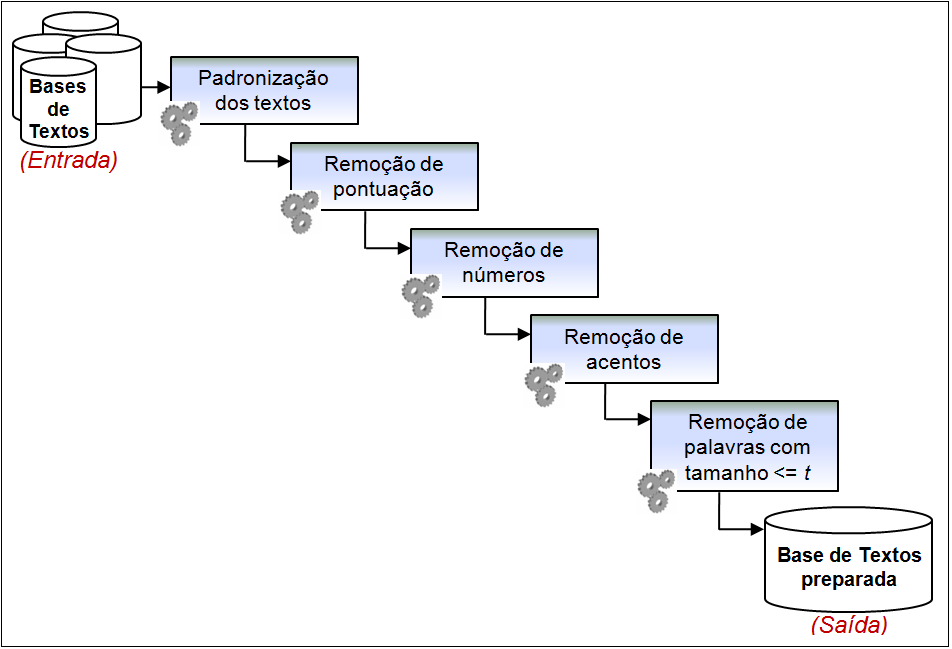
\includegraphics[scale=0.5]{figuras/fase1.png}
\caption{Prepara��o dos textos para a metodologia de extra��o de termos}
\label{fig:fase1}
\end{figure}

Considerando que os documentos podem vir de bases distintas, pode haver formatos diferentes de arquivos, sendo necess�rio a \textbf{padroniza��o dos textos}, colocando a base padronizada a ser trabalhada em um �nico reposit�rio.

A padroniza��o dos textos consiste em transformar todo o conte�do destes documentos para sua forma min�scula e padronizar os documentos para o formato de texto plano. Alguns documentos podem n�o permitir tal padroniza��o, por exemplo, o documento pode estar protegido contra c�pias ou estar em formato de figuras e imagens. Sendo assim, deve-se analisar subjetivamente o n�mero de documentos n�o danificados e, caso este n�mero seja considerado insuficiente, deve-se buscar por mais documentos. Todo o processo pode ser repetido at� se obter uma cole��o textual satisfat�ria para atingir os objetivos pr�-estabelecidos.
 
Em seguida, � realizada a \textbf{remo��o de pontua��o} dos textos, dado que a pontua��o somente aumentaria a quantidade de termos extra�dos, j� que os algoritmos utilizados na extra��o de termos n�o diferenciam pontua��o de palavras, extraindo, assim, termos compostos por pontua��es.

Pode-se tamb�m realizar a \textbf{remo��o de n�meros} dependendo do objetivo, ou seja, quando n�o � necess�rio trabalhar com n�meros nos textos. J� para a melhor compreens�o e jun��o das palavras iguais por t�cnicas pr�prias (como a radicaliza��o, a lematiza��o e a substantiva��o), � feita a \textbf{remo��o de acentos} das palavras dos textos.

\textbf{Remo��o de palavras com tamanho \textit{<= t}}, sendo \textit{t} o n�mero de caracteres de uma palavra. Tal remo��o � �til quando se tem caracteres sem nenhum significado, como por exemplo os caracteres \textit{z}, \textit{u} e \textit{rc}.

Na Tabela \ref{tab:doc_orig}, para melhor exemplificar as atividades da prepara��o dos textos, s�o mostrados dois par�grafos de um documento original da base de textos utilizada, como exemplo, neste trabalho. Na Tabela \ref{tab:doc_exe} s�o mostrados esses par�grafos preparados para serem utilizados, ou seja, o resultado dos mesmos ap�s a prepara��o dos textos seguindo os passos da fase 1 e ap�s a remo��o de \textit{stopwords}. Mesmo para apenas dois par�grafos de um documento, pode-se notar a redu��o do tamanho do mesmo, o que afeta a dimensionalidade da matriz atributo-valor. \\ \\

\begin{table}[!ht] \footnotesize \centering
\begin{tabular}{|c|} \hline
\\
\textit{``Em virtude dos bons resultados com animais em crescimento, os fazendeiros passaram} \\
\textit{alimentar com mistura de cana e ur�ia as vacas em lacta��o durante o per�odo seco do ano.''} \\ \\

\textit{``Nestes sistemas de pastejo extensivo de produ��o de leite, em que as vacas s�o} \\
\textit{alimentadas com cana-de-a��car e ur�ia, espera-se uma produ��o de leite elevada,} \\
\textit{n�o considerando o leite mamado pelo bezerro, al�m de ao final do per�odo seco} \\
\textit{as vacas apresentarem boa condi��o corporal e fertilidade adequada.''} \\ \\
\hline
\end{tabular}
\caption{Par�grafos retirados de um documento original da base de textos} \label{tab:doc_orig}
\end{table}



\begin{table}[!ht] \footnotesize \centering
\begin{tabular}{|c|} \hline
\\
\textit{virtude bons resultados animais crescimento fazendeiros passaram}\\ 
\textit{alimentar mistura cana ureia vacas lactacao periodo seco ano} \\  \\ 

\textit{sistemas pastejo extensivo producao leite vacas alimentadas cana acucar} \\ 
\textit{ureia esperase producao leite elevada considerando leite mamado bezerro} \\ 
\textit{final periodo seco vacas apresentarem boa condicao corporal fertilidade adequada} \\ \\
\hline
\end{tabular}
\caption{Par�grafos, referentes aos par�grafos mostrados na Tabela \ref{tab:doc_orig}, preparados para serem utilizados na metodologia de extra��o de termos} \label{tab:doc_exe}
\end{table}


Ap�s este passo, a base de textos a ser trabalhada � considerada preparada, permitindo, ent�o, efetuar a extra��o de termos de um dom�nio, que � explicada na Fase 2.



%----------------------------------------------------------------
%	Fase 2: Extra��o dos Termos
%----------------------------------------------------------------
\subsection{Fase 2: Extra��o dos Termos}
\label{extracao}

Dado o objetivo deste trabalho, que � avaliar o efeito do uso de diferentes formas de extra��o de termos, o processo proposto aqui faz uso de tr�s t�cnicas de simplifica��o de termos, descritas conceitualmente no Cap�tulo \ref{extracaoTermos}: a radicaliza��o por meio da ferramenta PreTexT II; a lematiza��o, usando a base de lemas do Lematizador de Nunes; e a substantiva��o, utilizando as ferramentas FORMA e CHAMA. Este processo pode ser estendido para outras diferentes t�cnicas.

O processo de extra��o de termos proposto, conforme ilustrado na Figura \ref{fig:fase2}, inicia-se com a base de textos considerada preparada para ser utilizada.

\begin{figure}[h]
\centering
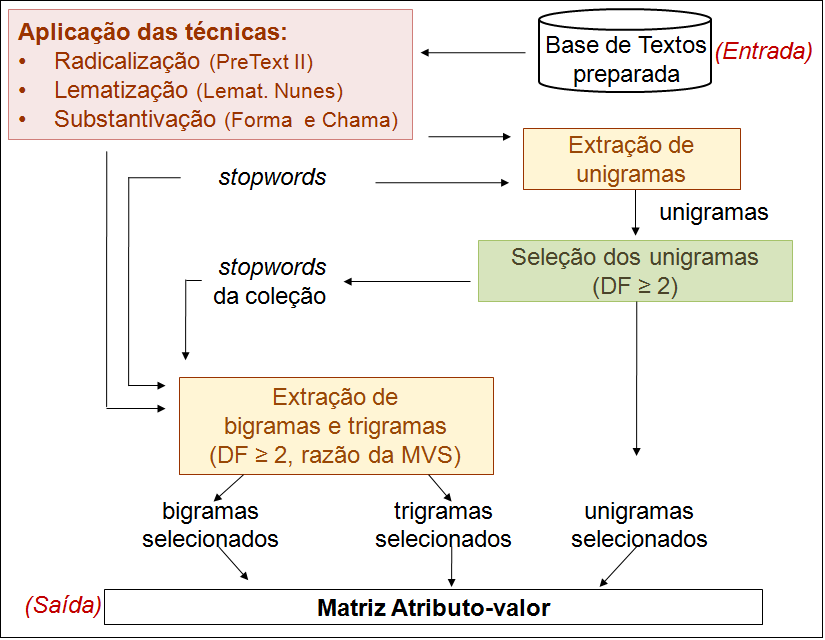
\includegraphics[width=1\textwidth]{figuras/fase2_v2.png}
\caption{Extra��o de termos}
\label{fig:fase2}
\end{figure}

O usu�rio pode escolher se deseja aplicar alguma t�cnica de simplifica��o de termos durante esta fase. Caso positivo, deve escolher qual t�cnica mais contribui para seu objetivo final. A seguir, s�o mostrados exemplos de palavras ap�s a aplica��o de cada uma destas t�cnicas, considerando como base os par�grafos de um documento mostrados na Tabela \ref{tab:doc_exe}.


Quando a t�cnica de radicaliza��o � aplicada, todas as palavras da cole��o de textos s�o transformadas em unigramas radicalizados com o uso da ferramenta PreTexT II. Essa transforma��o pode ser vista nas palavras que se encontram radicalizadas, que � mostrada na Tabela \ref{tab:palavras_radic}.%, sendo essas mostradas a seguir. \\ \\ \\

%\textit{\textbf{Palavras radicalizadas:}}

%\textit{virtud bom result anim cresciment fazende pass aliment mistur can ure vac lactaca period sec ano}

%\textit{sistem pastej extens produca leit vac aliment can acuc ure esperas produca leit elev consider leit mam bezerr final period sec vac apresent boa condica corporal fertil adequ} \\ \\

\begin{table}[!ht] \footnotesize \centering
\begin{tabular}{|c|} \hline
\\
\textit{virtud bom result anim cresciment fazende pass}\\ 
\textit{aliment mistur can ure vac lactaca period sec ano} \\  \\ 

\textit{sistem pastej extens produca leit vac aliment can acuc} \\ 
\textit{ure esperas produca leit elev consider leit mam bezerr} \\ 
\textit{final period sec vac apresent boa condica corporal fertil adequ} \\ \\
\hline
\end{tabular}
\caption{Palavras radicalizadas} \label{tab:palavras_radic}
\end{table}

Para a aplica��o da t�cnica de lematiza��o, utiliza-se a base de lemas do Lematizador de Nunes, que � composta por palavras na L�ngua Portuguesa e seus respectivos lemas. Como resultado, obt�m-se todas as palavras da cole��o de textos transformadas em palavras lematizadas, conforme mostrado na Tabela~\ref{tab:palavras_lemat}.%no exemplo a seguir. \\ \\


%\textit{\textbf{Palavras lematizadas:}}

%\textit{virtude resultado animal crescimento fazendeiro passar alimentar misturar cana ureia vaca lactacao periodo seco ano}

%\textit{sistema pastejo extensivo producao leite vaca alimentar cana acucar ureia esperase producao leite elevar considerar leite mamar bezerro alar final periodo seco vaca apresentar condicao corporal fertilidade adequar} \\ \\

\begin{table}[!ht] \footnotesize \centering
\begin{tabular}{|c|} \hline
\\
\textit{virtude resultado animal crescimento fazendeiro passar}\\ 
\textit{alimentar misturar cana ureia vaca lactacao periodo seco ano} \\  \\ 

\textit{sistema pastejo extensivo producao leite vaca alimentar cana acucar} \\ 
\textit{ureia esperase producao leite elevar considerar leite mamar bezerro} \\ 
\textit{alar final periodo seco vaca apresentar condicao corporal fertilidade adequar} \\ \\
\hline
\end{tabular}
\caption{Palavras lematizadas} \label{tab:palavras_lemat}
\end{table}

J� para a aplica��o da t�cnica de substantiva��o s�o utilizadas as ferramentas FORMA e CHAMA. Como resultado, tem-se todas as palavras transformadas para seus substantivos correspondentes, conforme mostrado na Tabela~\ref{tab:palavras_subst}.% A seguir, � mostrado um dessa transforma��o. \\ \\


%\textit{\textbf{Palavras substantivadas:}}

%\textit{virtude resultados animais crescimento fazendeiros passagem alimentar mistura cana ureia vacas lactacao periodo secura ano}

%\textit{sistemas pastejo extensividade producao leite vacas alimentacao cana acucar ureia esperase producao leite elevacao consideracao leite mamacao bezerro final periodo secura vacas apresentacao bondade condicao corporal fertilidade adequacao} \\ \\

\begin{table}[!ht] \footnotesize \centering
\begin{tabular}{|c|} \hline
\\
\textit{virtude resultados animais crescimento fazendeiros passagem}\\ 
\textit{alimentar mistura cana ureia vacas lactacao periodo secura ano} \\  \\ 

\textit{sistemas pastejo extensividade producao leite vacas alimentacao cana acucar} \\ 
\textit{ureia esperase producao leite elevacao consideracao leite mamacao bezerro} \\ 
\textit{final periodo secura vacas apresentacao bondade condicao corporal fertilidade adequacao} \\ \\
\hline
\end{tabular}
\caption{Palavras substantivadas} \label{tab:palavras_subst}
\end{table}

Para a obten��o de um documento substantivado, conforme mostrado na Figura \ref{fig:exe_forma_chama2}, na qual utiliza como exemplo de entrada as palavras \textit{vaca}, \textit{alimentadas} e \textit{cana}, primeiramente efetua-se a (a) aplica��o das ferramentas FORMA e CHAMA em cada palavra do texto. Esta aplica��o resulta em: \textit{<palavra\_original> <lema> <substantivo\_abstrato> <substantivo\_concreto> <classe\_gramatical>}. Cada palavra original do texto (indicada por \textit{<palavra\_original>}) � transformada para seu lema (\textit{<lema>}), bem como � gerado, a partir dessa palavra original, o substantivo abstrato correspondente a essa palavra (indicado por \textit{<substantivo\_abstrato>}). Gera-se tamb�m o correspondente substantivo concreto (\textit{<substantivo\_concreto>}) e indica-se a classe gramatical (<classe\_gramatical>) a qual a palavra original pertence.

Al�m disso, � colocada uma \textit{tag} em cada palavra original, sendo que neste caso as \textit{tags} colocadas foram: \_SUB (indica substantivo) e \_AP (indica partic�pio passado). O procedimento para a obten��o das palavras substantivadas desenvolvido neste trabalho e detalhado no Algoritmo \ref{ALG:meu_subst}, (b) considera como palavra substantivada o substantivo abstrato da palavra original, caso n�o possua, � considerado o substantivo concreto. Se as ferramentas n�o encontrarem nenhum destes substantivos, ent�o, � considerado o lema, j� que a substantiva��o de algumas das palavras originais corresponde ao seu pr�prio lema, como o caso das palavras \textit{vaca} e \textit{cana}.


\begin{figure} [h]
\centering
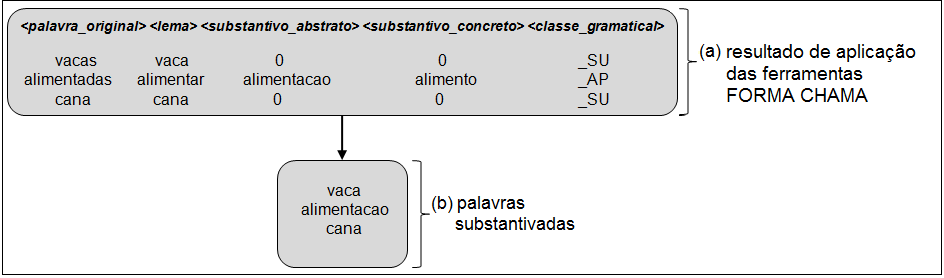
\includegraphics[width=1\textwidth]{figuras/exe_forma_chama2.png}
\caption{Exemplo da obten��o das palavras substantivadas}
\label{fig:exe_forma_chama2}
\end{figure}


\begin{algorithm}[h!]
\floatname{algorithm}{Algoritmo}	
	\caption{Substantiva��o das palavras da cole��o de textos}
	\label{ALG:meu_subst}
	\algsetup{indent=2em}
	\begin{algorithmic}[1]
	\REQUIRE cole��o de documentos original  $D$ $\{d_ 1, d_ 2,\ldots, d_ n\}$
	\ENSURE cole��o de documentos com palavras substantivadas  $Ds$
	\STATE $D \leftarrow \{d_ 1, d_ 2,\ldots, d_ n\}$
	\STATE $Ds \leftarrow \{ \}$
	
		\FORALL {$d_ i$  $\epsilon$  $D$}			
			\STATE $d'_ i \leftarrow$ aplica ferramentas FORMA e CHAMA $(d_ i)$
			\STATE $ds_ i \leftarrow$ pega palavras substantivadas $(d'_ i)$
		\ENDFOR
		
	\end{algorithmic}
\end{algorithm}




Ap�s a aplica��o das t�cnicas supra citadas, s�o geradas tr�s cole��es de textos contendo palavras simplificadas, uma cole��o para cada t�cnica. Para a obten��o de uma lista de unigramas a partir dessas palavras simplificadas, uma lista para cada cole��o textual, aplica-se, separadamente, a ferramenta PreTexT II, com a op��o de n�o radicalizar as palavras contidas nos documentos dessas cole��es.

Mesmo com a lista de unigramas contendo somente termos simplificados de acordo com cada t�cnica (uma lista para cada t�cnica separadamente) tem-se um elevado n�mero de unigramas, por�m nem todos representam positivamente os documentos. Para a \textbf{extra��o dos unigramas} mais representativos e os correspondentes \textit{n-gramas} que deles s�o derivados, pode-se considerar apenas os termos que aparecem, no m�nimo, em \textit{d} documentos na cole��o textual (\textit{\textbf{Document Frequency} - DF}), sendo que \textit{d} � fornecido pelo usu�rio e corresponde � quantidade m�nima de documentos no qual o termo deve aparecer. Al�m disso, remove-se uma lista de \textbf{\textit{stopwords}} padr�o para portugu�s (com artigos, interjei��es, etc). Ap�s a remo��o dos unigramas a partir da utiliza��o da \textit{Document Frequency} e da remo��o das \textit{stopwords}, obt�m-se os \textbf{unigramas selecionados}.

Em seguida, efetua-se a \textbf{extra��o dos \textit{n-gramas}} (bigramas e trigramas). Para isso, os unigramas que foram removidos a partir da \textit{Document Frequency} (ou qualquer outra medida que o usu�rio aplicar para remover os unigramas n�o representativos da cole��o) formam uma nova lista de termos, denominada \textbf{\textit{\-stoplist\-} da cole��o} - lista de \textit{stopwords} da cole��o.

A \textit{stoplist} da cole��o visa remover as palavras dos documentos que n�o s�o indicadas para formarem bons bigramas e trigramas, j� que estas palavras foram removidas na forma��o dos unigramas, o que indica que tal palavra n�o contribui para a representa��o da cole��o.

Assim, cada uma das t�cnicas de simplifica��o ter� uma lista de \textbf{bigramas} e uma lista de \textbf{trigramas selecionados}. Para exemplificar a diferen�a do uso de cada t�cnica na obten��o dessas combina��es (\textit{n-gramas}), a seguir s�o mostrados os trigramas extra�dos dos par�grafos de um documento exemplo apresentados na Tabela \ref{tab:doc_exe}. Os trigramas obtidos utilizando a t�cnica de radicaliza��o a partir desses par�grafos s�o mostrados na Tabela \ref{tab:tri_radic}.


\begin{table}[!ht] \footnotesize \centering
\begin{tabular}{|c c c|} \hline
& & \\
virtud\_bom\_result 			& period\_sec\_ano 				& elev\_consider\_leit \\
bom\_result\_anim 				& sistem\_pastej\_extens 	& consider\_leit\_mam \\
result\_anim\_cresciment 	& pastej\_extens\_produca & leit\_mam\_bezerr \\
anim\_cresciment\_fazende & extens\_produca\_leit 	& mam\_bezerr\_final \\
cresciment\_fazende\_pass & produca\_leit\_vac 			& bezerr\_final\_period \\
fazende\_pass\_aliment 		& leit\_vac\_aliment 			& final\_period\_sec \\
pass\_aliment\_mistur 		& vac\_aliment\_can 			& period\_sec\_vac \\
aliment\_mistur\_can 			& aliment\_can\_acuc 			& sec\_vac\_apresent \\
mistur\_can\_ure 					& can\_acuc\_ure 					& vac\_apresent\_boa \\
can\_ure\_vac 						& acuc\_ure\_esperas 			& apresent\_boa\_condica \\
ure\_vac\_lactaca 				& ure\_esperas\_produca 	& boa\_condica\_corporal \\
vac\_lactaca\_period 			& esperas\_produca\_leit 	& condica\_corporal\_fertil \\
lactaca\_period\_sec 			&  produca\_leit\_elev 		& corporal\_fertil\_adequ \\
													& leit\_elev\_consider & \\
& & \\
\hline
\end{tabular}
\caption{Trigramas obtidos com a t�cnica de radicaliza��o a partir dos par�grafos de um documento exemplo mostrados na Tabela \ref{tab:doc_orig}} \label{tab:tri_radic}
\end{table}



J� na Tabela \ref{tab:tri_lemat}, s�o apresentados os trigramas obtidos com a aplica��o da t�cnica de lematiza��o. Nota-se que as palavras \textit{\textbf{bons}} e \textit{\textbf{boa}}, ap�s a lematiza��o, correspondem a palavra \textit{\textbf{bom}}, sendo esta eliminada pela lista de \textit{stopwords} padr�o. Com isso os trigramas \textit{virtud\_bom\_result}, \textit{bom\_result\_anim}, \textit{vac\_apresent\_boa}, \textit{apresent\_boa\_condica} e \textit{boa\_condica\_corporal} n�o s�o constru�dos para a lematiza��o e sim, formam-se diferentes trigramas com a remo��o da palavra \textit{\textbf{bom}}, que s�o: \textit{virtude\_resultado\_animal} e \textit{apresentar\_condicao\_corporal}.


\begin{table}[!ht] \footnotesize \centering
\begin{tabular}{|c c c|} \hline
& & \\
virtude\_resultado\_animal 			& sistema\_pastejo\_extensivo		& leite\_elevar\_considerar \\
resultado\_animal\_crescimento	& pastejo\_extensivo\_producao	& elevar\_considerar\_leite \\
animal\_crescimento\_fazendeiro	& extensivo\_producao\_leite		& considerar\_leite\_mamar \\
crescimento\_fazendeiro\_passar	& producao\_leite\_vaca					& leite\_mamar\_bezerro \\
fazendeiro\_passar\_alimentar		& leite\_vaca\_alimentar				& mamar\_bezerro\_final \\
passar\_alimentar\_misturar			& vaca\_alimentar\_cana					& bezerro\_final\_periodo \\
alimentar\_misturar\_cana				& alimentar\_cana\_acucar				& final\_periodo\_seco \\
misturar\_cana\_ureia						& cana\_acucar\_ureia						& periodo\_seco\_vaca \\
cana\_ureia\_vaca								& acucar\_ureia\_esperase				& seco\_vaca\_apresentar \\
ureia\_vaca\_lactacao						& ureia\_esperase\_producao			& vaca\_apresentar\_condicao \\
vaca\_lactacao\_periodo					& esperase\_producao\_leite			& apresentar\_condicao\_corporal \\
lactacao\_periodo\_seco					& producao\_leite\_elevar				& condicao\_corporal\_fertilidade \\
periodo\_seco\_ano							&																& corporal\_fertilidade\_adequar \\
& & \\
\hline
\end{tabular}
\caption{Trigramas obtidos com a t�cnica de lematiza��o a partir dos par�grafos de um documento exemplo mostrados na Tabela \ref{tab:doc_orig}} \label{tab:tri_lemat}
\end{table}


Na Tabela \ref{tab:tri_subst}, � mostrado um exemplo dos trigramas obtidos utilizando a t�cnica de substantiva��o.


\begin{table}[!ht] \footnotesize \centering
\begin{tabular}{|c c c|} \hline
& & \\
virtude\_bons\_resultados 					& periodo\_secura\_ano							& elevacao\_consideracao\_leite \\
bons\_resultados\_animais						& sistemas\_pastejo\_extensividade	& consideracao\_leite\_mamacao \\
resultados\_animais\_crescimento		& pastejo\_extensividade\_producao	& leite\_mamacao\_bezerro \\
animais\_crescimento\_fazendeiros		& extensividade\_producao\_leite		& mamacao\_bezerro\_final \\
crescimento\_fazendeiros\_passagem	& producao\_leite\_vacas						& bezerro\_final\_periodo \\
fazendeiros\_passagem\_alimentar		& leite\_vacas\_alimentacao 				& final\_periodo\_secura \\
passagem\_alimentar\_mistura				& vacas\_alimentacao\_cana					& periodo\_secura\_vacas \\
alimentar\_mistura\_cana						& alimentacao\_cana\_acucar					& secura\_vacas\_apresentacao \\
mistura\_cana\_ureia								& cana\_acucar\_ureia 							& vacas\_apresentacao\_bondade \\
cana\_ureia\_vacas									& acucar\_ureia\_esperase						& apresentacao\_bondade\_condicao \\
ureia\_vacas\_lactacao							& ureia\_esperase\_producao					& bondade\_condicao\_corporal \\
vacas\_lactacao\_periodo						& esperase\_producao\_leite					& condicao\_corporal\_fertilidade \\
lactacao\_periodo\_secura						& producao\_leite\_elevacao					& corporal\_fertilidade\_adequacao \\
																		& leite\_elevacao\_consideracao			& \\
& & \\
\hline
\end{tabular}
\caption{Trigramas obtidos com a t�cnica de substantiva��o a partir dos par�grafos de um documento exemplo mostrados na Tabela \ref{tab:doc_orig}} \label{tab:tri_subst}
\end{table}


Devido ao elevado n�mero de combina��es obtidas (bigramas e trigramas) com a aplica��o de cada uma das t�cnicas de simplifica��o de termos, na tentativa de eliminar as combina��es que n�o representam muito a cole��o, s�o extra�das somente as combina��es de palavras que contenham na lista de unigramas finais. Para isso, � utilizada a \textit{stoplist} da cole��o, que � a lista de palavras eliminadas no processo de constru��o dos unigramas finais da cole��o. % ?? colocar exemplo da stoplist da cole��o ??

Mesmo assim, quando se trata de cole��es de textos de tamanhos elevados, o n�mero dessas combina��es (bigramas e trigramas) � ainda alto e grande parte delas n�o tem significado sem�ntico. Neste sentido, � necess�rio aplicar-lhes \textbf{m�todos estat�sticos}, como a medida (\textbf{\textit{Document Frequency} - DF}) e o \textbf{teste da raz�o de m�xima verossimilhan�a - MVS}.

O teste da raz�o de m�xima verossimilhan�a, dispon�vel no pacote NSP, visa detectar se as combina��es s�o mais do que simples co-ocorr�ncias casuais nos documentos, fornecendo, para isso, uma lista de todos os candidatos � combina��es. Segundo \citet{ManniSchut:2001} e \citet{GarraoDias:2008}, para a elabora��o desta lista (para o caso de bigramas $w^{1} w^{2}$, por exemplo), faz-se necess�rio a formula��o das duas hip�teses mostradas a seguir. Sendo que $H$ = hip�tese, $P$ = probabilidade e $w =$ palavra, que pertence � combina��o (grama).

\begin{center}
$H1: P (w^{1}| w^{2}) = P (w^{1}| \neg w^{2})$ \\
$H2: P (w^{1}| w^{2}) \neq P (w^{1}| \neg w^{2})$
\end{center}

A hip�tese 1 ($H1$) � a formaliza��o da independ�ncia, isto �, a ocorr�ncia de $w^{2}$ � independente da ocorr�ncia de $w^{1}$. A hip�tese 2 ($H2$) � a formaliza��o da depend�ncia, e quando ela � satisfeita significa que pode ter sido encontrada uma combina��o interessante.

Por exemplo, assumindo que o bigrama \textit{cana\_acucar} � uma combina��o, tem-se:

\begin{center}
$H2:P(cana|acucar) \neq P(cana|\neg acucar)$ \\
$H1:P(cana|acucar) = P(cana|\neg acucar)$
\end{center}

Espera-se que a hip�tese de independ�ncia $H1$ seja falsa, indicando que provavelmente foi encontrada uma combina��o interessante.

O resultado da aplica��o deste teste � um \textit{rank} dos \textit{n-gramas} em ordem decrescente de import�ncia de acordo com o valor obtido pelo teste para cada \textit{n-grama}. Considerando ainda o documento utilizado como exemplo anteriormente, na Tabela \ref{tab:teste_ll}, s�o listados alguns dos bigramas e trigramas obtidos com o uso da t�cnica de radicaliza��o a partir de tal documento, juntamente com as respectivas freq��ncias no documento e os valores do teste da raz�o de m�xima verossimilhan�a. Segundo os valores desse teste, o termo \textit{sistem\_pastej\_extens} � considerado como mais importante do que o termo \textit{leit\_vac}.


\begin{table}[!ht] \footnotesize \centering
\begin{tabular}{|c|c|c|} \hline
\textit{N-gramas}				& Freq��ncias	& Valores do teste\\ \hline \hline
sistem\_pastej\_extens	& 4						& 18.9027 \\ \hline
sistem\_pastej					& 3 					& 9.4990 \\ \hline
pastej\_extens					& 3 					& 9.4990 \\ \hline
can\_acuc								& 4 					& 6.7264 \\ \hline
vac\_aliment						& 7 					& 3.0061 \\ \hline
leit\_vac							& 8 					& 2.0609 \\ \hline
\end{tabular}
\caption{Exemplos dos valores obtidos pela aplica��o do teste da raz�o de m�xima verossimilhan�a para alguns bigramas e trigramas} \label{tab:teste_ll}
\end{table}


Por fim, a base de textos, agora representada pelos termos extra�dos da mesma, � estruturada em uma \textbf{matriz atributo-valor}, na qual o documento a que o termo pertence � colocado como linha da matriz, os termos extra�dos como co\-lu\-nas, e a matriz � preenchida, neste caso, com a freq��ncia absoluta deste termo no respectivo documento. Deve-se ressaltar que o sucesso de tarefas de Extra��o de Padr�es � diretamente afetado pela qualidade dos termos que comp�em esta matriz. Ressalta-se, portanto, a import�ncia de se obter termos representativos do dom�nio, sendo, ent�o, necess�rio escolher uma t�cnica adequada para a extra��o desses termos.



%%%%%%%%%%%%%%%%%%%%%%%%%%%%%%%%%%%%%%%%%%%%%%%%%%%%%%%%%%%%%%%%%
%   Ferramenta ExtraT
%%%%%%%%%%%%%%%%%%%%%%%%%%%%%%%%%%%%%%%%%%%%%%%%%%%%%%%%%%%%%%%%%

\section{Ferramenta ExtraT}
Para a aplica��o da metodologia de extra��o de termos proposta aqui foi desenvolvida uma ferramenta denominada ExtraT (Ferramenta para Extra��o de Termos) utilizando a linguagem de programa��o Java juntamente com o ambiente integrado para desenvolvimento de software Eclipse\footnote{Eclipse - http://www.eclipse.org/platform} Vers�o 3.3.2. Para a aplica��o da t�cnica de lematiza��o utiliza-se a base de palavras e seus respectivos lemas contidos no Lematizador de Nunes. Na aplica��o da t�cnica de substantiva��o s�o utilizadas conjuntamente as ferramentas FORMA e CHAMA. J� para a aplica��o da radicaliza��o e a obten��o dos \textit{n-gramas}, independente de qual t�cnica o usu�rio escolher, � utilizada a ferramenta PreTexT II. Por fim, a aplica��o do m�todo estat�stico do teste da raz�o de m�ximo verossimilhan�a faz uso do pacote NSP.

A op��o por utilizar a PreTexT � devido ao fato que esta, ao contr�rio das outras ferramentas de radicaliza��o, possibilita tamb�m a combina��o dos \textit{stems} (\textit{n-gramas}). J� a escolha pelo uso do Lematizador de Nunes � que este apresentou bons resultados em trabalhos anteriores, como no trabalho de \citet{AleixoPardo:2008}. Al�m disso, o FLANOM foi desenvolvido somente para a L�ngua Espanhola e o software Sphinx � propriet�rio. Quanto ao uso dos etiquetadores morfossint�ticos citados, n�o � interessante utiliz�-los para auxiliar na aplica��o da lematiza��o devido a necessidade de se aplicar outra ferramenta para lematizar o resultado destes etiquetadores.

Deve-se ressaltar que o trabalho aqui proposto tem um maior foco na abordagem estat�stica j� que, segundo \citet{Teline:2003}, o uso de m�todos ling��sticos t�m como conseq��ncia sua aplica��o somente a uma l�ngua e, �s vezes, at� mesmo a uma �nica variante. Por�m, a t�cnica de radicaliza��o, por exemplo, pode ser aplicada em outras diversas l�nguas al�m do Portugu�s, j� a substantiva��o, encontrada na literatura, s� � aplic�vel � L�ngua Portuguesa. Tanto as \textit{stopwords}, que podem ser obtidas ou constru�das para outras l�nguas, quanto o \textit{thesaurus}, ambos utilizados neste trabalho, est�o inseridos na abordagem ling��stica. O \textit{thesaurus} � utilizado na abordagem proposta de avalia��o de termos extra�dos, explicada no Cap�tulo \ref{avaliacao}.

Dentro da abordagem estat�stica, este trabalho faz uso do teste da raz�o de m�xima verossimilhan�a que visa indicar se um termo candidato � uma boa coloca��o para ser utilizada na cole��o de textos em quest�o. Este teste foi escolhido para ser utilizado pois, segundo \citet{ManniSchut:2001}, � o mais adequado para ser utilizado quando se trabalha com dados bastante esparsos, que � o caso da Minera��o de Textos. Al�m disso, o estimador $\chi^2$ � menos recomendado para trabalhar com cole��es textuais pequenas e � menos interpret�vel, se comparado ao teste raz�o de m�xima verossimilhan�a, pois este �ltimo fornece um \textit{ranking}, n�o sendo necess�rio utilizar uma tabela, como no $\chi^2$ \citep{MantelEtAl:1985}.

Esta ferramenta permite que o usu�rio execute a extra��o de termos utilizando diferentes t�cnicas de simplifica��o dos termos para bases de textos da sua escolha. Os passos para essa execu��o seguem as fases desta metodologia conforme descritas neste cap�tulo. Na Figura \ref{fig:extrat}(a) � ilustrada a especifica��o dos diret�rios de entrada e sa�da escolhidos pelo usu�rio, ou seja, como diret�rio de entrada tem-se as bases de textos que o usu�rio deseja processar e o diret�rio de sa�da corresponde ao diret�rio que o usu�rio deseja que sejam gerados os resultados do processamento.

%\begin{figure} [h]
%\centering
%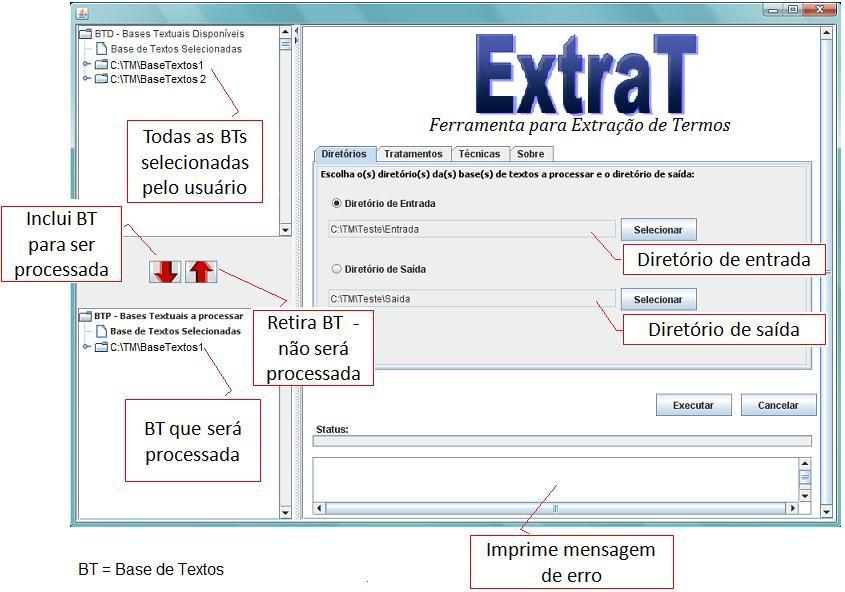
\includegraphics[width=15cm,height=5cm]{figuras/tela1.jpg}
%\caption{Escolha de diret�rios na ferramenta ExtraT}
%\label{fig:tela1}
%\end{figure}


A primeira fase da metodologia, que � a prepara��o dos textos, pode ser executada na ferramenta ExtraT conforme mostrada na Figura \ref{fig:extrat}(b), e a segunda fase da metodologia, que � a extra��o dos termos � ilustrada na Figura \ref{fig:extrat}(c).


%\begin{figure} [h]
%\centering
%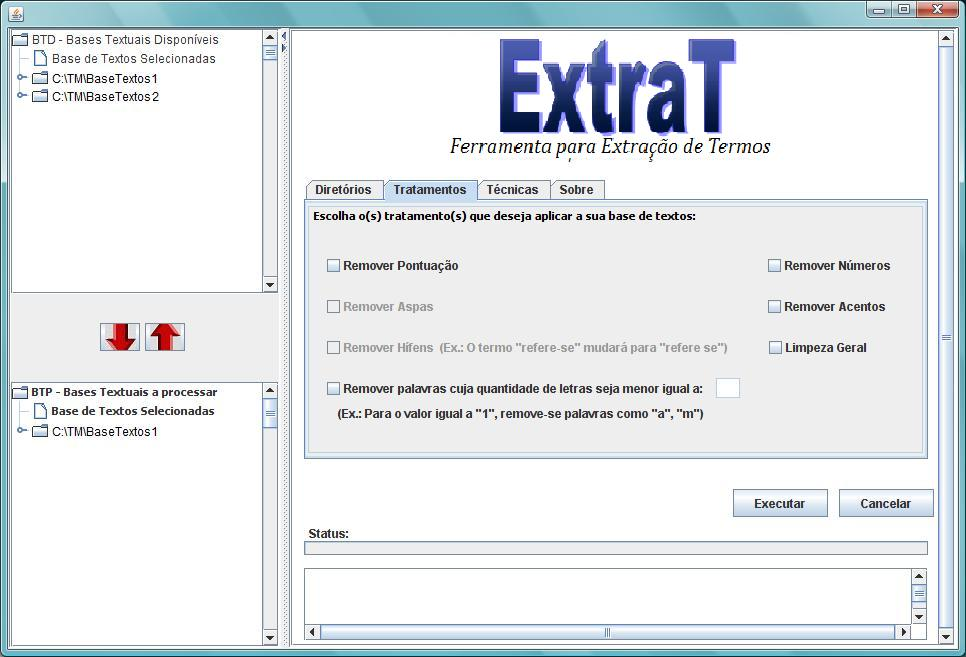
\includegraphics[width=14.5cm,height=5cm]{figuras/tela2.jpg}
%\caption{Prepara��o dos textos na ferramenta ExtraT}
%\label{fig:tela2}
%\end{figure}
%
%
%\begin{figure} [h]
%\centering
%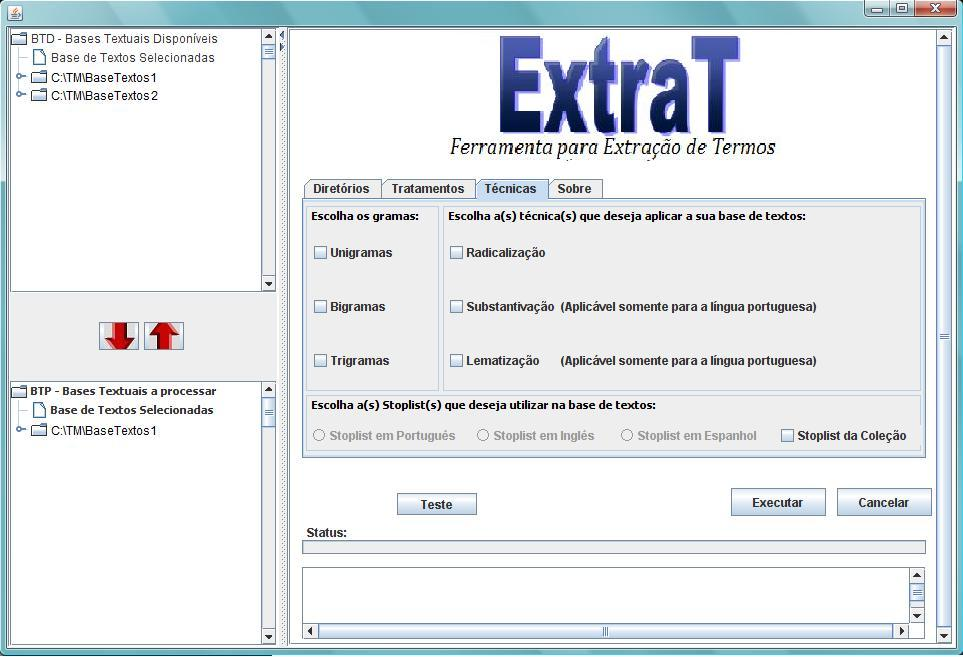
\includegraphics[width=14.5cm,height=5cm]{figuras/tela3.jpg}
%\caption{Extra��o dos termos na ferramenta ExtraT}
%\label{fig:tela3}
%\end{figure}


\begin{figure}
\center
\subfigure[a][Escolha de diret�rios na ferramenta ExtraT]{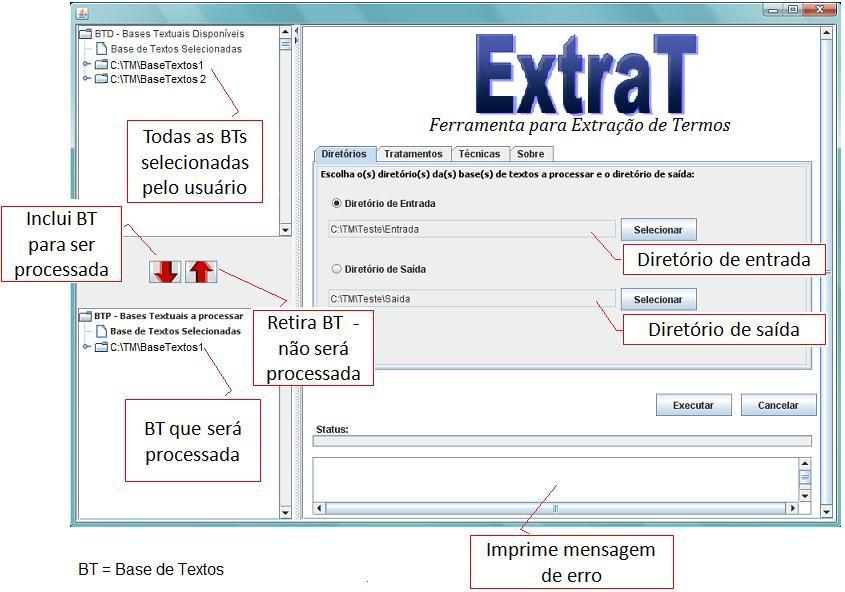
\includegraphics[scale=0.45]{figuras/tela1.jpg}}\\
\subfigure[b][Prepara��o dos textos na ferramenta ExtraT]{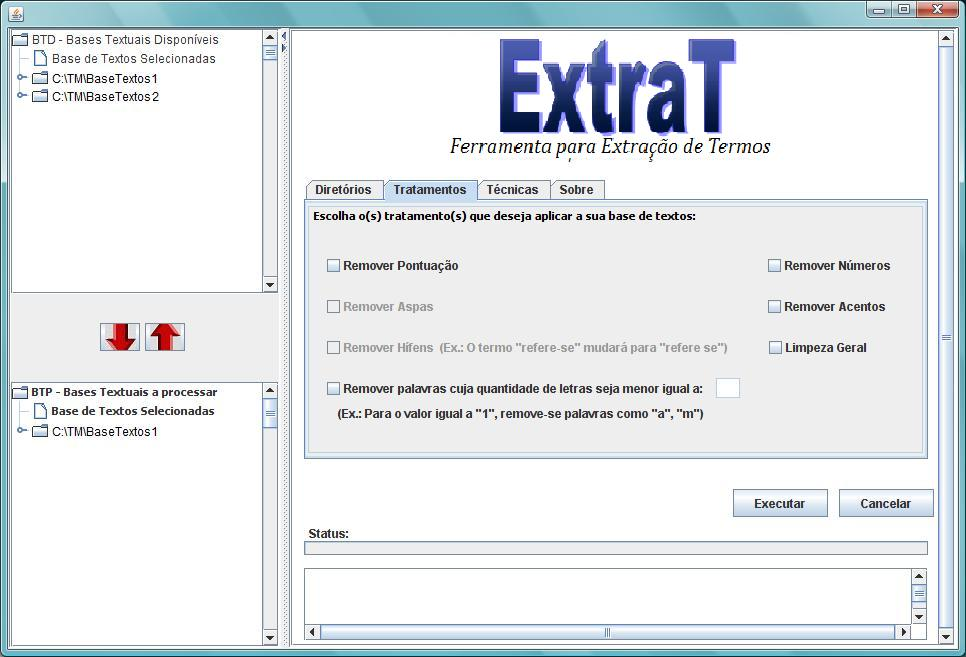
\includegraphics[scale=0.4]{figuras/tela2.jpg}}\\
\subfigure[c][Extra��o dos termos na ferramenta ExtraT]{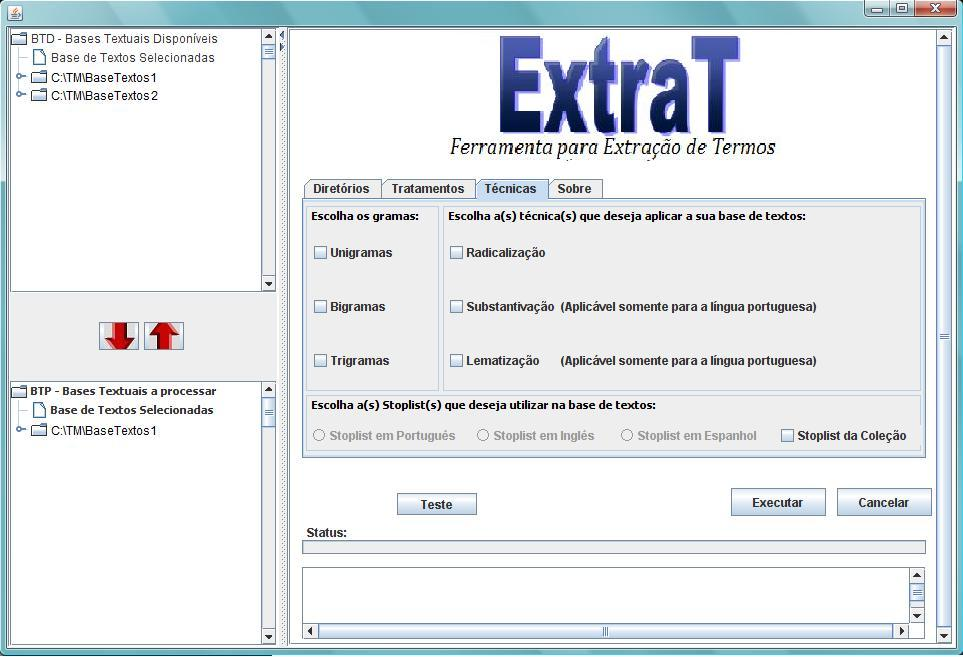
\includegraphics[scale=0.4]{figuras/tela3.jpg}}\\
\caption{Ferramenta para extra��o de termos - ExtraT}
\label{fig:extrat}
\end{figure}

%%%%%%%%%%%%%%%%%%%%%%%%%%%%%%%%%%%%%%%%%%%%%%%%%%%%%%%%%%%%%%%%%
%   Contribui��es Finais
%%%%%%%%%%%%%%%%%%%%%%%%%%%%%%%%%%%%%%%%%%%%%%%%%%%%%%%%%%%%%%%%%
\newpage
\pagebreak[4]
\section{Considera��es Finais}

Neste cap�tulo foi descrita a metodologia para a aplica��o de diferentes formas de extra��o de termos a partir de cole��es textuais de dom�nio espec�fico, bem como a ferramenta ExtraT, que foi desenvolvida para apoiar a utiliza��o de tal metodologia. Essas diferentes formas englobam a utiliza��o de tr�s t�cnicas que simplificam os termos extra�dos: a radicaliza��o, a substantiva��o e a lematiza��o.

Esta metodologia engloba duas fases, que � a prepara��o dos documentos da base de textos da qual � trabalhada e a extra��o dos termos utilizando as t�cnicas anteriormente citadas. Ap�s a obten��o dos termos extra�dos, estes devem ser avaliados garantindo que seu uso contribua positivamente para atingir os objetivos pr�-estabelecidos pelo usu�rio. Sendo assim, neste trabalho tamb�m � proposta uma abordagem de avalia��o, descrita no Cap�tulo \ref{avaliacao}, que faz uso de taxonomias \textit{gold} e a medida de avalia��o de termos CTW (\textit{Context Term Weight}). Al�m disso, a metodologia de extra��o de termos pode ser estendida para outras t�cnicas de simplifica��o de termos al�m das tr�s supra citadas que foram encontradas na literatura.


\chapter{Avalia��o dos Termos Extra�dos}
\label{avaliacao}
%   5.1 Considera��es Iniciais
%		5.2 Descri��o da Forma de Avalia��o dos Termos Extra�dos
%				5.2.1 Avalia��es Subjetivas dos Termos Gerados
%				5.2.2 Avalia��es Objetivas dos Termos Gerados
%		5.3 Avalia��es
%				5.3.1 Descri��o do Avalia��o
%				5.3.2 Bases de Textos Utilizadas
%				5.3.3 Discuss�o dos Resultados
%   4.6 Considera��es Finais

%%%%%%%%%%%%%%%%%%%%%%%%%%%%%%%%%%%%%%%%%%%%%%%%%%%%%%%%%%%%%%%%%
%   Considera��es Iniciais
%%%%%%%%%%%%%%%%%%%%%%%%%%%%%%%%%%%%%%%%%%%%%%%%%%%%%%%%%%%%%%%%%

\section{Considera��es Iniciais}
Na avalia��o dos termos extra�dos � verificado se os resultados obtidos est�o em conformidade com os resultados esperados por meio de avalia��es subjetivas e objetivas. Tanto para as avalia��es subjetivas como para uma avalia��o objetiva, faz-se uso de taxonomias \textit{gold}. Neste trabalho, as taxonomias \textit{gold} s�o taxonomias de refer�ncias, ou seja, s�o consideradas como taxonomias validadas e que podem ser utilizadas como modelo para experimentos. Como exemplo de trabalho que utilizou taxonomias \textit{gold} para avalia��o, pode-se citar o trabalho de \citet{KaEtAl:2005}.

Neste cap�tulo tamb�m � descrita a avalia��o experimental realizada utilizando os passos da metodologia de extra��o de termos detalhada no Cap�tulo \ref{abordExtracao}. Para esse experimento realizado foram feitas sete avalia��es, englobando avalia��es subjetivas, conforme descrito na Se��o \ref{avalSubjetiva}; e avalia��es objetivas, de acordo com a descri��o da Se��o \ref{avalObjetiva}. S�o apresentados os resultados obtidos nessa avalia��o experimental e as an�lises dos mesmos. O experimento tem como objetivo avaliar as formas de extra��o de termos em um dom�nio espec�fico. Al�m de apontar, por meio de avalia��es subjetivas e objetivas, algumas das caracter�sticas positivas e negativas da utiliza��o das t�cnicas de simplifica��o de termos (radicaliza��o, lematiza��o e substantiva��o), quando a compreensibilidade, a representatividade e a quantidade de termos t�m impacto direto na interpreta��o e uso dos resultados.


%%%%%%%%%%%%%%%%%%%%%%%%%%%%%%%%%%%%%%%%%%%%%%%%%%%%%%%%%%%%%%%%%
%   Descri��o das Formas de Avalia��o dos Termos Extra�dos
%%%%%%%%%%%%%%%%%%%%%%%%%%%%%%%%%%%%%%%%%%%%%%%%%%%%%%%%%%%%%%%%%

\section{Abordagem para Avalia��o dos Termos Extra�dos}
\label{formas_avaliacao}
Os termos extra�dos a partir de cole��es de textos podem ser utilizados para diversos fins, al�m de seu uso em taxonomias do dom�nio. Como o foco deste trabalho � avaliar diferentes formas de extra��o de termos de um dom�nio espec�fico, sendo que estas diferentes formas correspondem ao uso principalmente de tr�s t�cnicas de simplifica��o de termos (radicaliza��o, lematiza��o e substantiva��o), deve-se avaliar a compreensibilidade dos mesmos, j� que cada t�cnica de simplifica��o trabalha com m�todos diferentes, extraindo, portanto, termos distintos. Tamb�m � importante avaliar se os termos extra�dos correspondem ao dom�nio em quest�o.

Neste trabalho, a ``qualidade'' dos termos extra�dos abrange tanto a representatividade dos termos no dom�nio como sua compreensibilidade. Neste sentido, para avaliar os termos extra�dos s�o feitas algumas avalia��es subjetivas e objetivas em rela��o ao dom�nio em quest�o, considerando cada uma das t�cnicas de simplifica��o de termos separadamente. As avalia��es subjetivas, ou seja, com o aux�lio de especialistas, abrangem: (i) a representatividade dos termos em seus respectivos documentos; (ii) a compreensibilidade dos termos obtidos ao utilizar cada t�cnica; e (iii) a prefer�ncia geral subjetiva dos especialistas em cada t�cnica. Como exemplo de avalia��o subjetiva pode-se citar o trabalho de \citet{ConradoEtAl:2009}, no qual foram feitas avalia��es semelhantes para o dom�nio de Intelig�ncia Artificial. No trabalho de \citet{ConEtAl:2009} tamb�m foram feitas avalia��es subjetivas, bem como objetivas, ambas voltadas para termos do dom�nio de agroneg�cio.

As avalia��es objetivas levam em considera��o (iv) a quantidade de termos extra�dos por cada t�cnica, al�m de abranger tamb�m (v) a representatividade dos termos extra�dos a partir de cada t�cnica em rela��o aos seus respectivos documentos.

Ap�s feitas todas estas avalia��es, considera-se ser poss�vel ressaltar caracter�sticas positivas e negativas da utiliza��o das t�cnicas de simplifica��o de termos.


%----------------------------------------------------------------
%		Avalia��es Subjetivas dos Termos Extra�dos
%----------------------------------------------------------------
\subsection{Avalia��es Subjetivas dos Termos Extra�dos}
\label{avalSubjetiva}
As avalia��es subjetivas dos termos extra�dos tem como objetivo avaliar (i) o qu�o bem os termos extra�dos representam seus respectivos textos, considerando cada uma das t�cnicas; (ii) a compreensibilidade dos termos extra�dos ao utilizar cada t�cnica de simplifica��o de termos; e (iii) a prefer�ncia geral subjetiva dos especialistas em rela��o �s t�cnicas.
 
Para que tais avalia��es sejam poss�veis, s�o efetuados tr�s passos: (1) a \textbf{gera��o de taxonomias de t�picos utilizando as diferentes t�cnicas de simplifica��o de termos}, em seguida, � feita uma (2) \textbf{an�lise subjetiva das taxonomias por especialistas do dom�nio}, com uma forma clara de apresenta��o dos termos extra�dos, permitindo avaliar qual forma � mais adequada para apoiar os es\-pe\-ci\-a\-lis\-tas do dom�nio em seus objetivos e possibilitar a implementa��o de melhorias na abordagem como um todo. Ap�s esta an�lise, � efetuado um (3) \textbf{c�lculo de precis�o da representatividade dos termos} extra�dos em rela��o ao dom�nio em quest�o. Estes tr�s passos s�o explicados detalhadamente a seguir.

%Por fim, o conhecimento gerado (taxonomia gerada) pode ser finalmente utilizado para o objetivo pr�-estabelecido pelo usu�rio.
 

%----------------------------------------------------------------
%		Passo 1: Gera��o de taxonomias de t�picos utilizando as diferentes formas de gera��o de termos
%----------------------------------------------------------------
\subsubsection{Passo 1: Gera��o de taxonomias de t�picos utilizando as diferentes t�cnicas de simplifica��o de termos}
A metodologia para constru��o de taxonomias de t�picos proposta em \citet{ConradoWTI:2008} � aplicada �s cole��es de textos. Cada cole��o � pr�-processada e os termos representantes da mesma s�o extra�dos utilizando separadamente as t�cnicas de simplifica��o de termos (radicaliza��o, lematiza��o e substantiva��o), conforme detalhado no Cap�tulo \ref{extracaoTermos}. Dessa forma, trabalha-se com tr�s conjuntos de termos representados por suas respectivas matriz atributo-valor, sendo que o primeiro conjunto cont�m termos radicalizados; o segundo � composto por termos lematizados; e o terceiro cont�m termos substantivados.

Para a gera��o das taxonomias, durante a etapa de Extra��o de Padr�es, para cada conjunto de termos, utiliza-se o algoritmo de agrupamento hier�rquico \textit{average-link} sobre cada matriz atributo-valor dos conjuntos de termos. Uma vez obtido um agrupamento hier�rquico para cada conjunto de termos, as taxonomias s�o geradas a partir da rotula��o da hierarquia, na qual s�o considerados os termos mais freq�entes. Os termos s�o selecionados e ordenados de acordo com sua freq��ncia em cada grupo de documentos.

Desta forma, para cada cole��o textual s�o obtidas tr�s vers�es de taxonomias com a mesma estrutura hier�rquica, por�m rotuladas com os termos obtidos em cada t�cnica de simplifica��o, conforme ilustrado na Figura \ref{fig:exemplo_taxonomias}.

\begin{figure} [h]
\centering
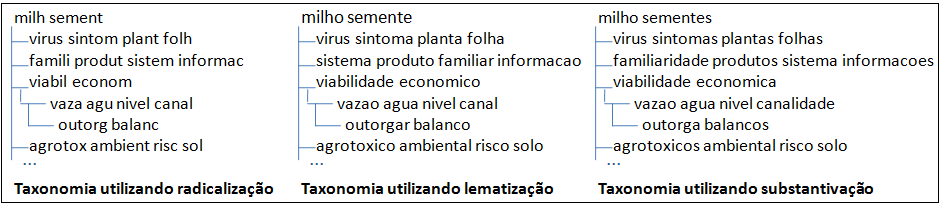
\includegraphics[width=1\textwidth]{figuras/exemplo_taxonomias.png}
\caption{Exemplo de taxonomias com a mesma estrutura hier�rquica utilizando as diferentes t�cnicas de simplifica��o de termos}
\label{fig:exemplo_taxonomias}
\end{figure}


Devido � exist�ncia da mesma estrutura hier�rquica das taxonomias, para cada conjunto de termos, � poss�vel selecionar ramos que representam um mesmo grupo de documentos para avalia��o. Isto permite que os usu�rios comparem a compreensibilidade dos termos utilizados nos r�tulos de cada grupo sobre um mesmo cen�rio, uma vez que o mesmo conceito � apresentado em cada grupo. Al�m disso, espera-se que bons grupos sejam compactos de modo que seus documentos apresentem alta similaridade, enquanto que a similaridade com os elementos de outros grupos seja a menor poss�vel. Neste caso, a similaridade foi calculada utilizando a dist�ncia de cosseno.

Como as taxonomias geradas podem possuir um tamanho elevado para serem avaliadas subjetivamente pelos especialistas, s�o selecionados os 10 (dez) grupos da hierarquia que apresentam a menor variabilidade interna da similaridade entre os documentos (os grupos mais coesos) para facilitar a an�lise subjetiva do conceito representado naquele grupo por parte dos especialistas e permitir a avalia��o da qualidade dos termos ali selecionados.


%----------------------------------------------------------------
%		Passo 2: An�lise subjetiva das taxonomias por especialistas do dom�nio
%----------------------------------------------------------------
\subsubsection{Passo 2: An�lise subjetiva das taxonomias por especialistas do dom�nio}
Como o objetivo deste trabalho n�o � a gera��o de taxonomias e, sim de termos, n�o � considerada a avalia��o de taxonomias em si, pois para isso seria necess�rio uma pesquisa abrangente sobre as formas e m�todos dispon�veis para gera��o das mesmas. Por isso, neste trabalho as taxonomias s�o utilizadas para auxiliar a avalia��o dos termos extra�dos.

Sendo assim, com o aux�lio da ferramenta TaxTools \citep{MarcaciniRezende:2008}, os especialistas do dom�nio em quest�o devem avaliar os ramos escolhidos das taxonomias obtidas e examinar os documentos e descritores (termos) obtidos, sendo que a partir de cada observa��o, os especialistas devem eleger uma nota ao ramo, entre um (1) e quatro (4) correspondente a:

\begin{enumerate}
 	\item Nota 1 - Muito ruim, termos nada discriminativos  	
	\item Nota 2 - Termos pouco discriminativos 	
	\item Nota 3 - Termos bem discriminativos 	
	\item Nota 4 - Termos muito bons
\end{enumerate} 

Esta nota diz respeito a representatividade subjetiva dos termos em rela��o ao dom�nio em quest�o, isto �, o qu�o os termos extra�dos representam seus respectivos documentos.

Em seguida, passa-se para a segunda parte da avalia��o, conforme ilustrado na Figura \ref{fig:notasNoh}. A quest�o (a) avalia a compreensibilidade dos termos, ou seja, qual (ou quais) t�cnica obteve termos mais compreens�veis - f�ceis de serem entendidos pelos especialistas (usu�rios finais dos termos). A quest�o (b) avalia qual das t�cnicas os especialistas consideram como a mais adequada para ser utilizada na cole��o textual no dom�nio.

\begin{figure} [h]
\centering
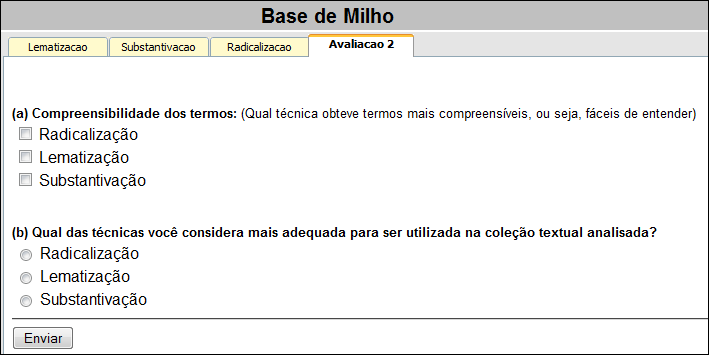
\includegraphics[width=1\textwidth]{figuras/notasNoh.png}
\caption{Avalia��o do ramo selecionado}
\label{fig:notasNoh}
\end{figure}


Assim, considera-se ser poss�vel avaliar os termos extra�dos de acordo com a compreensibilidade dos mesmos a partir da an�lise dos especialistas do dom�nio e ainda por sua prefer�ncia por utilizar alguma das t�cnicas.

%----------------------------------------------------------------
%		Passo 3: C�lculo da representatividade e compreensibilidade dos termos
%----------------------------------------------------------------
\subsubsection{Passo 3: C�lculo da representatividade e compreensibilidade dos termos}

As notas atribu�das pelos especialistas s�o tabuladas de acordo com as notas dadas nos ramos em cada taxonomia de cada cole��o textual. Dessa forma, � poss�vel realizar testes comparativos, com base em an�lise de vari�ncia das notas em fun��o de cada um dos efeitos envolvidos na avalia��o, que s�o: em rela��o ao ramo (n�) avaliado; em rela��o �s diferentes t�cnicas de simplifica��o de termos utilizadas; e em rela��o ao avaliador.

Estes testes comparativos s�o realizados por meio de compara��es m�ltiplas de m�dias, indicando se h� ou n�o diferen�a estatisticamente significativa entre as m�dias de cada t�cnica utilizada. Com isso, � poss�vel indicar se alguma t�cnica obteve resultados melhores nestes testes em rela��o �s outras.


%----------------------------------------------------------------
%		Avalia��es Objetivas da Extra��o de Termos
%----------------------------------------------------------------
\subsection{Avalia��es Objetivas dos Termos Extra�dos}
\label{avalObjetiva}
A quantidade de termos extra�dos com o uso de diferentes t�cnicas de simplifica��o de termos (radicaliza��o, lematiza��o e substantiva��o), utilizando a mesma base de textos, � diferente para cada t�cnica. Neste sentido, � necess�rio considerar na avalia��o dos termos, al�m da compreensibilidade e representatividade dos termos, (iv) a quantidade de termos extra�dos por cada t�cnica.% Por�m, deve-se tamb�m considerar o tempo de execu��o em que cada t�cnica utiliza para gerar os termos.

Para avaliar objetivamente (v) a representatividade dos termos extra�dos a partir de cada t�cnica separadamente em rela��o a um determinado dom�nio, � utilizado um vocabul�rio expandido do mesmo dom�nio.

Foram escolhidas, para caso de uso, algumas �rvores publicadas pela Ag�ncia de Informa��o Embrapa\footnote{Ag�ncia de Informa��o Embrapa - http://www.agencia.cnptia.embrapa.br/} como taxonomias \textit{gold}. Devido a algumas diferen�as entre formas de armazenamento dos dados da Ag�ncia e dos dados no ambiente TopTax, foi feita uma prepara��o dos dados das Ag�ncias de Informa��o Embrapa para o padr�o necess�rio � compara��o com o vocabul�rio automaticamente obtido. Ressalta-se que, em trabalhos futuros, esta prepara��o poder� ser utilizada para auxiliar na avalia��o autom�tica de taxonomias de t�picos automaticamente geradas contra taxonomias de t�picos \textit{gold}. Essa avalia��o poder� ser efetuada comparando-se, por exemplo, cada um dos t�picos de uma taxonomia gerada automaticamente com cada um dos t�picos de uma taxonomia \textit{gold}, assim, poder-se-� avaliar a rotula��o feita para a gera��o da taxonomia, bem como os termos contidos em cada t�pico da mesma.

Para melhor compreens�o dos passos necess�rios para a avalia��o objetiva dos termos e, possivelmente, de taxonomias de dom�nios espec�ficos, � detalhada a taxonomia utilizada do dom�nio de agroneg�cio, que � a taxonomia de t�picos da Ag�ncia de Informa��o Embrapa. Bem como, s�o descritas a adapta��o desta taxonomia para ser utilizada como base na avalia��o (taxonomia \textit{gold}) com a utiliza��o do Thesagro, e as duas poss�veis formas de avalia��o dispon�veis com esse processo.

A escolha pela utiliza��o do Thesagro � devida ao fato que este atende �s necessidades da metodologia de avalia��o apresentada aqui. Tais necessidades s�o: (i) a obten��o de um vocabul�rio expandido; e (ii) o uso de bases de textos do mesmo dom�nio do vocabul�rio expandido. Nesse sentido, como tem-se dispon�veis as bases de textos do dom�nio de agroneg�cio e o Thesagro, que � do dom�nio agr�cola validado e consolidado, torna-se vi�vel e interessante o seu uso.

%----------------------------------------------------------------
%		A Taxonomia de T�picos da Ag�ncia de Informa��o EMBRAPA
%----------------------------------------------------------------
\subsubsection{A Taxonomia de T�picos da Ag�ncia de Informa��o Embrapa}
Uma das formas de divulga��o de informa��o na Embrapa � a Ag�ncia de Informa��o, que ``� um sistema Web que possibilita a organiza��o, o tratamento, o armazenamento, a divulga��o e o acesso � informa��o tecnol�gica e ao conhecimento gerados pela Embrapa e outras institui��es de pesquisa''\footnote{Ag�ncia de Informa��o Embrapa - http://www.agencia.cnptia.embrapa.br/}  \citep{SouzaEtAl:2006}.
%Esta refer�ncia est� com erro em seu formato:
%@INPROCEEDINGS{SouzaEtAl:2006,
%  author = {SOUZA, M. I. F. and SANTOS, A. D. dos and MOURA, Maria Fernanda.
%	and ALVES, M. das D. R.},
%  title = {Ag�ncia de Informa��o Embrapa: uma aplica��o para a organiza��o da
%	informa��o e gest�o do conhecimento},
%  booktitle = {Simp�sio Brasileiro de Engenharia de Software e Simp�sio Brasileiro
%	de Bancos de Dados - Workshop de Bibliotecas Digitais},
%  year = {2006},
%  editor = {Anais... Florian�polis: SBC},
%  pages = {51--56},
%  owner = {Merley},
%  timestamp = {2009.05.12}
%}


Os dados e informa��es contidos na Ag�ncia s�o organizados em hierarquias, denominadas �rvores do conhecimento. Nos primeiros n�veis das hierarquias est�o os conhecimentos mais gen�ricos e, nos n�veis mais profundos, est�o os conhecimentos espec�ficos \citep{Evangelista:2003}. Cada n� da hierarquia corresponde a um tema (t�pico) descrito por um texto, que resulta da compila��o do conhecimento produzido por pesquisadores, t�cnicos extensionistas e agricultores; e, ainda faz refer�ncias a outras obras que complementam essa informa��o. Tais hierarquias s�o visualizadas por meio de �rvores hiperb�licas ou navega��o por hipertexto das p�ginas Web. Adicionalmente, s�o fornecidas ferramentas de busca alimentadas por palavras-chave.

Utilizar �rvores da Ag�ncia de Informa��o Embrapa como taxonomias \textit{gold} � interessante, uma vez que a informa��o � p�blica, consolidada, validada e completa. Mesmo assim, algumas adapta��es foram necess�rias, devido �s caracter�sticas das taxonomias envolvidas no processo.% Tais caracter�sticas diz respeito � constru��o manual das �rvores, sendo que estas devem ser comparadas �s taxonomias automaticamente geradas.

A primeira caracter�stica � que para cada n�, em uma taxonomia de t�picos automaticamente obtida, o t�pico possui um ou mais termos como palavras-chave a serem validadas, e cada um desses termos possui termos similares, que poderiam ter sido tamb�m automaticamente encontrados. Na �rvore de conhecimento da Ag�ncia, cada n� � representado apenas pelos termos mais espec�ficos,  que foram subjetivamente selecionados a partir de um \textit{thesaurus}. Por exemplo, o termo \textit{Abacaxi}, neste dom�nio, poderia tamb�m ser representado pelo termo \textit{Ananas Comosus}, assim, o n� deveria conter os termos \textit{Abacaxi} e \textit{Ananas Comosus}. Dessa forma, para comparar a taxonomia automaticamente gerada com uma \textit{gold}, sem perda de informa��o, foi necess�rio expandir os termos em cada n� das �rvores da Ag�ncia, buscando termos sin�nimos e/ou relacionados no \textit{thesaurus} utilizado, no caso, o Thesagro (\textit{Thesaurus} Nacional Agr�cola).

A segunda caracter�stica � que, taxonomias automaticamente obtidas agrupam documentos em t�picos, e, a seguir procuram palavras-chave para descrever os t�picos nesses documentos. Na Ag�ncia, em cada n� da hierarquia h� uma p�gina Web contendo uma s�ntese assunto do n� em quest�o e, possivelmente mais documentos relacionados ao n� s�o referenciados, bem como metadados desses documentos. Novamente, uma adapta��o faz-se necess�ria, a fim de abstrair esses textos como documentos agrupados sob o n�. 


%----------------------------------------------------------------
%		Adapta��o da �rvores da Ag�ncia a uma Taxonomia Gold
%----------------------------------------------------------------
\subsubsection{Adapta��o da �rvores da Ag�ncia a uma Taxonomia \textit{Gold} }
O processo de obten��o autom�tica de taxonomias de t�picos necessita da extra��o de termos capazes de representar com qualidade cada n�. Al�m disso, esses termos podem e devem ser utilizados como palavras-chave dos documentos, podendo alimentar express�es de busca na cole��o de textos ou em cole��es similares. Deve-se ressaltar que, n�o necessariamente, esses termos representam adequadamente o dom�nio de conhecimento completo, pois s�o obtidos a partir de uma cole��o restrita de documentos.

Adicionalmente, espera-se que o volume de termos extra�dos automaticamente da cole��o seja maior do que um conjunto de termos selecionados por humanos em um \textit{thesaurus}.  Assim, para avaliar a ``qualidade'' dos termos extra�dos das mesmas cole��es de documentos que geraram algumas �rvores da Ag�ncia, implementaram-se os processos de adapta��o de algumas �rvores da Ag�ncia a uma taxonomia \textit{gold}. Para efetuar as adapta��es foi desenvolvida a ferramenta TaXEm (Taxonomia em XML da Embrapa), que utiliza como base de vocabul�rio controlado o contido no Thesagro. Deve-se ressaltar que, apenas Ag�ncias de produto foram utilizadas, a fim de garantir que o \textit{thesaurus} utilizado fosse  o Thesagro; dado que essas �rvores s�o baseadas em cadeia produtiva de produtos agr�colas.

Conforme apresentado na Figura \ref{fig:taxem}, o processo de adapta��o proposto neste trabalho consiste em: a partir dos arquivos que armazenam a estrutura hier�rquica das Ag�ncias, reestrutur�-la de modo que seja poss�vel facilmente vincular os documentos relacionados a cada n�; e que, cada n� seja rotulado com os termos que o representam, viabilizando uma busca mais ampla.

\begin{figure}[ht]
    \centering
        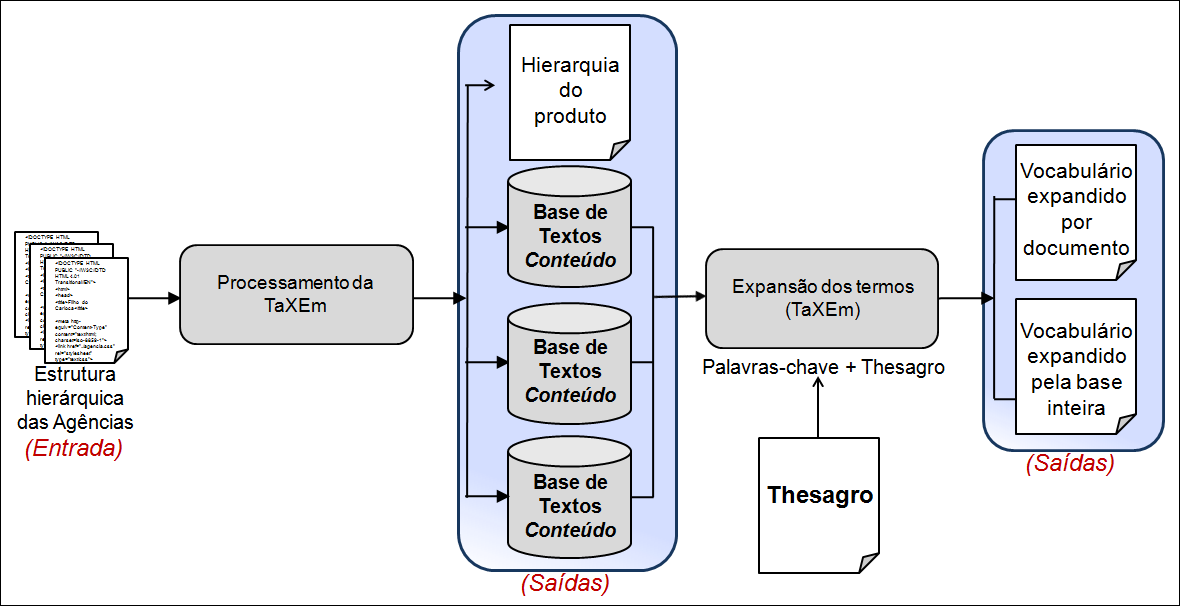
\includegraphics[scale=0.38]{figuras/taxem.png}
    \caption{Processo para a prepara��o do conte�do das Ag�ncias}
    \label{fig:taxem}
\end{figure}

Assim, para cada entrada, a hierarquia dos n�s para o produto � preparada em formato \textit{.xml}, e em cada n�, os documentos relativos ao mesmo s�o referenciados. Estes documentos s�o gerados em formato de texto plano em tr�s diferentes categorias: \textit{conte�do}, \textit{mais detalhes} e \textit{recursos}. Os documentos pertencentes � categoria \textit{conte�do} descrevem o t�pico, nos moldes da Ag�ncia; os documentos da categoria \textit{mais detalhes} s�o os metadados sobre os recursos; e os pertencentes a \textit{recursos} s�o os pr�prios recursos dispon�veis do n�, isto �, as informa��es complementares citadas no texto que descreve o n�.

Os termos originais da hierarquia s�o expandidos com a utiliza��o do Thesagro, isto �, s�o aumentadas as possibilidades de cada palavra-chave acrescentando-lhes sin�nimos ou termos relacionados. As rela��es existentes no Thesagro foram explicadas mais detalhadamente na Se��o \ref{vocabControlado} do Cap�tulo \ref{extracaoTermos}. Utilizando a nota��o do Thesagro, na expans�o de cada termo \textit{T} (descritor), consideraram-se os termos relacionados (\textit{RT}) ao termo buscado \textit{T}; sendo que, os \textit{RT} possuem significados que se relacionam semanticamente com o termo \textit{T}, mas sem nenhuma liga��o hier�rquica entre si. Tamb�m s�o considerados os termos que possuem alguma rela��o de equival�ncia (denominados\textit{USE}), que s�o classificados, neste trabalho, como os termos que possuem alguma rela��o de equival�ncia ao termo \textit{T}. Na Figura \ref{fig:thesagro} s�o mostrados exemplos de (a) \textit{RT} e (b) \textit{USE}. O termo (descritor) \textit{enologia} possui um significado sem�ntico relacionado ao termo (\textit{RT}) \textit{vinho}, e o termo (descritor) \textit{abacaxizeiro} possui uma rela��o de equival�ncia com o termo \textit{abacaxi}, ou seja, o termo \textit{abacaxizeiro} pode ser usado (\textit{USE}) como \textit{abacaxi}.

\begin{figure}[ht]
    \centering
        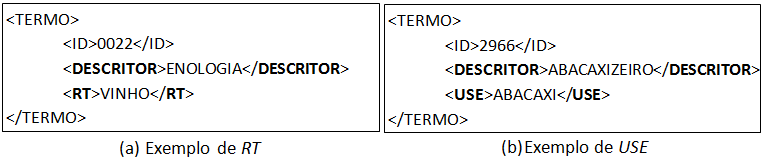
\includegraphics[scale=0.58]{figuras/thesagro.png}
    \caption{Exemplos de \textit{\textbf{RT}} e \textit{\textbf{USE}}}
    \label{fig:thesagro}
\end{figure}

O vocabul�rio expandido, obtido com a utiliza��o do Thesagro, � apresentado de duas formas: (a) separado por documento e (b) referente � base inteira, conforme ilustrado na Figura \ref{fig:vocabulario}.

\begin{figure}[ht]
    \centering
        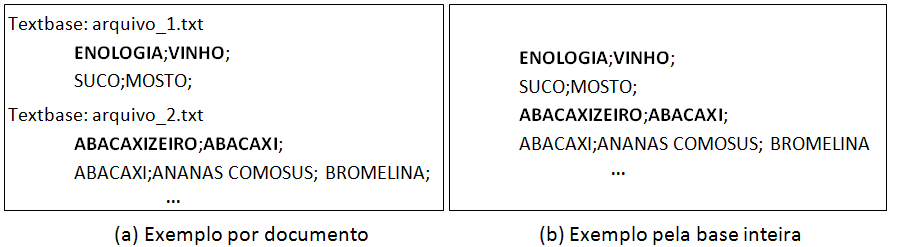
\includegraphics[scale=0.5]{figuras/vocabulario.png}
    \caption{Vocabul�rio expandido}
    \label{fig:vocabulario}
\end{figure}

%----------------------------------------------------------------
%		Formas de Avalia��o Objetiva dos Termos Extra�dos
%----------------------------------------------------------------
\subsubsection{Formas de Avalia��o Objetiva dos Termos Extra�dos}
A primeira forma de avalia��o objetiva visa analisar objetivamente a representatividade dos termos extra�dos em rela��o ao dom�nio da cole��o de textos que os mesmos foram extra�dos. Para isso, utilizou-se como suporte a medida CTW (\textit{Context Term Weight}) \citep{MayAnan:1999}, que avalia a quantidade de vezes (a freq��ncia do termo na cole��o) em que um termo extra�do aparece em um determinado contexto. Neste caso, o contexto � representado por um vocabul�rio expandido obtido pela TaXEm, ou seja, os termos representativos e consagrados do dom�nio juntamente com seus sin�nimos, que s�o obtidos do Thesagro. Sendo assim, para a avalia��o dos termos, os mesmos s�o recuperados no vocabul�rio expandido. A descri��o formal da medida CTW (\textit{Context Term Weight}) adaptada para este trabalho �:

\begin{equation}
CT(a) = \sum_{d \epsilon T_a} f_a (d)
\end{equation}

\noindent no qual $a$ � o termo extra�do seguindo os passos da metodologia de extra��o de termos apresentada neste trabalho; $T_a$ � o conjunto das palavras do vocabul�rio expandido que coincidem com os termos extra�dos; $d$ � a palavra de $T_a$; e $f_a (d)$ � a freq��ncia de $d$ como um termo $a$, que � obtida durante a extra��o de termos seguindo os passos da metodologia apresentada neste trabalho.

Na Tabela \ref{tab:exe_ctw} � mostrado um exemplo do uso da medida CTW (\textit{Context Term Weight}) neste trabalho. Neste exemplo, a pontua��o CTW � igual a 30, que � obtida somente a partir das freq��ncias do termos \textit{abacaxi} (20) e \textit{ananas} (10), pois o termo \textit{ruim} n�o est� presente no vocabul�rio expandido, n�o sendo, portanto, considerado como um termo importante para o dom�nio do vocabul�rio.


\begin{table}[h] 
\centering \footnotesize
\begin{tabular}{|c|c|c|c|} 
\hline
\multicolumn{2}{|c|}{\bf \it Termos extra�dos}
																&	\multirow{2}{*}{\bf \it Termos do vocabul�rio expandido} 	& \multirow{2}{*}{\bf \it Pontua��o da CTW} \\ \cline{1-2}
Termos ($a$)	& Freq��ncias ($f_a$)														&																										& \\ \hline \hline
abacaxi				&	20																						& abacaxi, ananas, abacaxizeiro.										& \multirow{3}{*}{30} \\
ananas				& 10																						&	ma��, macieira.																		& \\
ruim					&	5																							&																										& \\ \hline
\end{tabular}
\caption{Exemplo do uso da medida CTW neste trabalho} \label{tab:exe_ctw}
\end{table}


Al�m disso, com o aux�lio da TaXEm � poss�vel haver uma segunda forma de avalia��o objetiva, na qual considera como base a taxonomia \textit{gold}, com o objetivo de verificar se os termos extra�dos representam os t�picos e sub-t�picos do dom�nio. Dessa forma, as compara��es podem ser feitas verificando os termos de cada n� em cada hierarquia ou verificando a posi��o dos n�s das hierarquias. Isso � poss�vel devido ao padr�o da hierarquia preparada na TaXEm, o que permite sua f�cil visualiza��o, utilizando, por exemplo, a ferramenta TaxTools \citep{MarcaciniRezende:2008}, como ilustrada na Figura \ref{fig:hierarquias} que usa como exemplo o produto Feij�o, conforme publicado na Ag�ncia Embrapa. Nesta figura � mostrada (a) a hierarquia da �rvore do Feij�o reestruturada pela TaXEm contendo somente os termos originais e (b) a mesma hierarquia contendo os termos expandidos com o vocabul�rio.

\begin{figure}[ht]
    \centering
        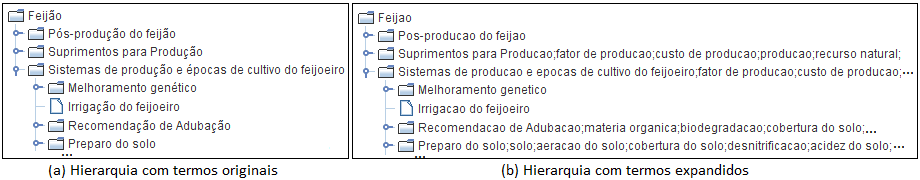
\includegraphics[scale=0.5]{figuras/hierarquias.png}
    \caption{Exemplo da visualiza��o da hierarquia}
    \label{fig:hierarquias}
\end{figure}

Como nesta segunda forma de avalia��o, cada n� da taxonomia \textit{gold} � comparado com o n� da taxonomia obtida. Nesta avalia��o, considera-se os termos extra�dos, a forma como foi gerada a taxonomia com tais termos, como a rotula��o utilizada em cada uma, j� que este pode afetar a posi��o de cada n� e, conseq�entemente, se o resultado obtido desta avalia��o foi afetado por isso. Devido ao foco deste trabalho, n�o ser� considerada esta segunda forma de avalia��o.



%----------------------------------------------------------------
%   Bases de Textos Utilizadas
%----------------------------------------------------------------
\section{Bases de Textos Utilizadas}
As bases de textos a ser utilizadas podem vir de qualquer dom�nio, pois tal metodologia de extra��o termos apresentada neste trabalho � independente do dom�nio. Para experimento, foram utilizadas bases de textos reais dispon�veis na Embrapa, devido � necessidade de possuir os textos das bases e seus respectivos termos originais para poder avaliar se os termos aqui extra�dos obtiveram resultados satisfat�rios.

Para a avalia��o objetiva dos termos extra�dos, foi necess�rio utilizar um \textit{thesaurus} do mesmo dom�nio das bases de textos, sendo assim, houve um refor�o positivo pela escolha destas bases, pois seu dom�nio � o mesmo do dom�nio do \textit{thesaurus} dispon�vel (o Thesagro). Dessa forma, o experimento foi conduzido utilizando oito bases de textos na L�ngua Portuguesa referentes a oito produtos diferentes cultivados na Embrapa. A quantidade de documentos destas bases � mostrada na Tabela~\ref{tab:todasBases}. Estas bases foram pr�-processadas, conforme descri��o do Cap�tulo \ref{pre_processamento}, e, como conseq��ncia, alguns documentos foram removidos por n�o estarem adequados para a extra��o de termos. Portanto, a quantidade de documentos de algumas bases foi diminu�da (documentos finais).


\begin{table}[!ht]
\centering \scriptsize
\begin{tabular}{|l|c|c|c|c|}
\hline
\raisebox{0.0ex}[0pt][0pt]{\bf \it \textbf{Base de Textos (Produto)}} & {\bf \it \textbf{\# Docs Iniciais}} &
 {\bf \it \textbf{\# Docs Finais}} & \bf \it \textbf{M�dia de palavras por texto}
\\
\hline \hline
\textit{Milho} & 511 & 510 & 705.04\\
\hline
\textit{Cana} & 431 & 391 & 1272.81\\
\hline
\textit{Feij�o} & 352 & 348 & 801.63\\
\hline
\textit{Leite} & 332 & 332 & 278.40\\
\hline
\textit{Ma��} & 231 & 230 & 895.97\\
\hline
\textit{Caupi} & 204 & 198 & 1933.70\\
\hline
\textit{Eucalipto} & 100 & 100 & 277.20\\
\hline
\textit{Caju} & 40 & 40 & 531.50\\
\hline

\end{tabular}
\caption{Descri��o das bases de textos} \label{tab:todasBases}
\end{table}
% perda no num de docs, pois alguns n�o converteram de .pdf para .txt (texto plano) e outros eram .wmv


%----------------------------------------------------------------
%   Avalia��o Experimental
%----------------------------------------------------------------
\section{Avalia��o Experimental}
%Sendo assim, na avalia��o dos termos � considerada a quantidade de termos gerados por cada t�cnica utilizando a abordagem proposta neste trabalho e descrita na Se��o~\ref{abordExtracao}. Adicionalmente, para comparar...


Os termos foram extra�dos a partir de cole��es textuais do dom�nio de agroneg�cio de tr�s diferentes formas. Essa extra��o seguiu os passos da metodologia descrita no Cap�tulo \ref{abordExtracao}. Ressaltando que cortes, como Luhn e Salton, n�o foram utilizados no experimento deste trabalho, mesmo que a metodologia apresentada aqui possibilita o uso dos mesmos. Tal escolha tem o objetivo de diminuir a subjetividade da metodologia, j� que estes exigem que sejam fornecidos os pontos de corte.

A primeira forma de extra��o de termos utilizou para a simplifica��o dos termos a t�cnica de radicaliza��o; a segunda forma fez uso da t�cnica de lematiza��o; e a terceira utilizou a t�cnica de substantiva��o. As avalia��es s�o descritos a seguir.


%---------------------- Avalia��o 1
\subsection{Avalia��o 1 - O uso da Metodologia de Extra��o de Termos Proposta}

\textbf{Objetivo:} verificar se a extra��o de termos seguindo os passos descritos na metodologia de extra��o de termos contribui consideravelmente para a diminui��o da quantidade de termos, j� que esta � um problema existente no processo de Minera��o de Textos.

\textbf{Hip�tese:} a extra��o de termos seguindo os passos descritos na metodologia de extra��o de termos contribui consideravelmente para a diminui��o da quantidade de termos.

\textbf{Descri��o:} primeiramente, para cada base de textos e t�cnica utilizada para a extra��o de termos, foram extra�dos (a) os \textit{termos iniciais} (unigramas, bigramas e trigramas), removendo-se somente a lista de \textit{stopwords} padr�o para portugu�s dispon�vel na PreTexT, as conjuga��es do verbo SER e as palavras compostas por apenas um caracter. Logo em seguida, foram extra�dos (b) os termos finais, que foram obtidos seguindo os passos da metodologia descrita no Cap�tulo \ref{abordExtracao}. Para a extra��o dos termos finais, foram considerados apenas os termos que aparecem, no m�nimo, em dois documentos na cole��o textual (\textit{Document Frequency} - $DF>= 2$); e para o teste da raz�o de m�xima verossimilhan�a adotou-se $p\_value = 0.05$, visando manter somente os bigramas e trigramas que contenham algum significado sem�ntico.

Com a extra��o de \textit{termos iniciais} e \textit{finais} separadamente � poss�vel observar a redu��o da quantidade de termos obtida quando a extra��o de termos � feita seguindo os passos da metodologia proposta neste trabalho, ou seja, quando se trabalha com os termos finais. Tal redu��o, utilizando as tr�s t�cnicas de simplifica��o de termos separadamente, � mostrada nas Figuras \ref{fig:num_termos_radic}, \ref{fig:num_termos_lemat} e \ref{fig:num_termos_subst}; e as quantidades \textit{iniciais} e \textit{finais} de unigramas, bigramas e trigramas extra�dos (n�mero de termos e porcentagem de redu��o) s�o mostradas na Tabela \ref{tab:quant_termos}. A porcentagem de redu��o mostrada nessa Tabela, diz respeito ao percentual de redu��o da quantidade de termos quando comparado o total de \textit{termos iniciais (a)} com o total de \textit{termos finais (b)} referentes � cada t�cnica.


\begin{figure}
\centering
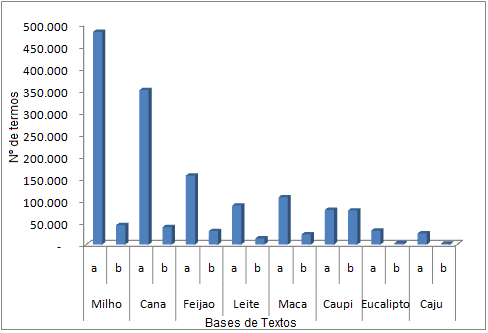
\includegraphics[width=14.5cm,height=6cm]{figuras/num_termos_radic.png}
\caption{Redu��o do n�mero de termos utilizando a t�cnica de radicaliza��o}
\label{fig:num_termos_radic}
\end{figure}


\begin{figure}
\centering
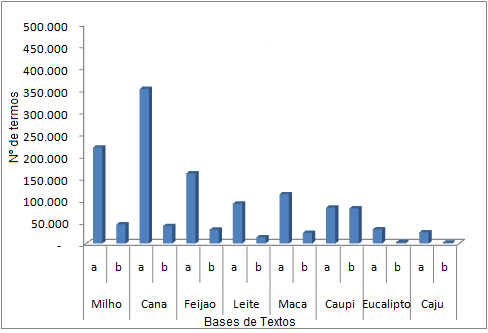
\includegraphics[width=14.5cm,height=6cm]{figuras/num_termos_lemat.png}
\caption{Redu��o do n�mero de termos utilizando a t�cnica de lematiza��o}
\label{fig:num_termos_lemat}
\end{figure}


\begin{figure}
\centering
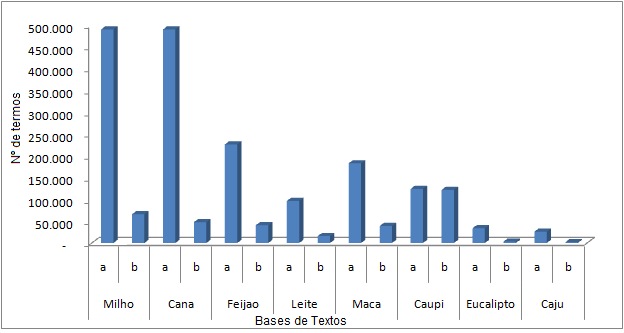
\includegraphics[width=14cm,height=6cm]{figuras/num_termos_subst.png}
\caption{Redu��o do n�mero de termos utilizando a t�cnica de substantiva��o}
\label{fig:num_termos_subst}
\end{figure}


%\definecolor{gray1}{gray}{.85}
%\definecolor{gray2}{gray}{.70}
%\cellcolor[gray]{0.8} - \rowcolor[gray]{.9} - \colorbox{gray2}{...}

\begin{table}[!ht]
\centering \footnotesize
\begin{tabular}{|c|c|c|c|c|c|c|c|}
\hline

	& &\multicolumn{2}{|c|}{\bf \textit{Radicaliza��o}} & \multicolumn{2}{|c|}{\bf \textit{Lematiza��o}} & \multicolumn{2}{|c|}{\bf \textit{Substantiva��o}} \\ \hline
\bf \textit{Bases}							&	\bf \textit{Gramas} &	  (a) 	&	 (b)   &   (a) 	&	  (b)   &	  (a) 	&	 (b)   \\ \hline \hline

\multirow{5}{*}{\bf \textsl{Milho}}			&	Unigramas 	&	19.883  & 6.526	 & 15.791  & 6.934  & 23.556  & 7.744  \\ \cline{2-8}
																				&	Bigramas 		&	167.412 & 15.838 & 93.603  & 21.548 & 197.077 & 28.884 \\ \cline{2-8}
																				&	Trigramas 	& 295.105 & 21.808 & 109.478 & 15.107 & 270.678 & 29.543 \\ \cline{2-8}
																				&	{\bf Total} & 482.400 & 44.172 & 218.872 & \textcolor{blue}{43.589} & 491.311 & 66.171 \\ \cline{2-8}
	& {\bf \% Redu��o$*$} & \multicolumn{2}{|c|}{\bf 91\%} & \multicolumn{2}{|c|}{\bf 80\%} & \multicolumn{2}{|c|}{\bf 87\%} \\ \hline \hline
\multirow{4}{*}{\bf \textsl{Cana}}			&	Unigramas 	&	20.249 	& 8.316  & 21.960  & 8.697  & 23.556 	& 9.501  \\ \cline{2-8}
																				&	Bigramas 		& 177.858 & 21.019 & 153.088 & 21.067 & 197.077 & 24.785 \\ \cline{2-8}
																				&	Trigramas 	& 152.414 & 10.157 & 177.460 & 10.197 & 270.678 & 13.738 \\ \cline{2-8}
																				&	{\bf Total} & 350.521 & \textcolor{blue}{39.492} & 352.508 & 39.961 & 491.311 & 48.024 \\ \cline{2-8}
	& {\bf \% Redu��o$*$} & \multicolumn{2}{|c|}{\bf 89\%} & \multicolumn{2}{|c|}{\bf 89\%} & \multicolumn{2}{|c|}{\bf 90\%} \\ \hline \hline
\multirow{4}{*}{\bf \textsl{Feij�o}}		&	Unigramas &	10.542 	& 5.401  & 11.631  & 5.798  & 12.599 	& 6.243  \\ \cline{2-8}
																				&	Bigramas 		&	78.915 	& 14.321 & 67.835  & 14.572 & 88.311 	& 17.993 \\ \cline{2-8}
																				&	Trigramas 	& 66.881 	& 10.918 & 80.585  & 11.233 & 125.817 & 16.652 \\ \cline{2-8}
																				&	{\bf Total} & 156.338 & \textcolor{blue}{30.640} & 160.051 & 31.603 & 226.727 & 40.888 \\ \cline{2-8}
	& {\bf \% Redu��o$*$} & \multicolumn{2}{|c|}{\bf 80\%} & \multicolumn{2}{|c|}{\bf 80\%} & \multicolumn{2}{|c|}{\bf 82\%} \\ \hline \hline
\multirow{4}{*}{\bf \textsl{Leite}}			&	Unigramas 	& 5.419 	& 3.051  & 6.403 	 & 3.454  & 6.568 	& 3.524  \\ \cline{2-8}
																				&	Bigramas 		&	36.948 	& 6.663  & 37.936  & 6.681  & 40.228 	& 7.257  \\ \cline{2-8}
																				&	Trigramas 	& 46.210 	& 4.130  & 46.789  & 4.132  & 49.807 	& 5.127  \\ \cline{2-8}
																				&	{\bf Total} & 88.577 	& \textcolor{blue}{13.844} & 91.128  & 14.267 & 96.603 	& 15.908 \\ \cline{2-8}
	& {\bf \% Redu��o$*$} & \multicolumn{2}{|c|}{\bf 84\%} & \multicolumn{2}{|c|}{\bf 84\%} & \multicolumn{2}{|c|}{\bf 84\%} \\ \hline \hline
\multirow{4}{*}{\bf \textsl{Ma��}}			&	Unigramas 	& 7.988 	& 4.537  & 9.412 	 & 5.174  & 9.595 	& 5.225  \\ \cline{2-8}
																				&	Bigramas 		&	51.661 	& 12.075 & 53.863  & 12.426 & 74.347 	& 17.556 \\ \cline{2-8}
																				&	Trigramas 	& 47.723 	& 6.545  & 49.115  & 6.654  & 99.375 	& 16.284 \\ \cline{2-8}
																				&	{\bf Total} & 107.372 & \textcolor{blue}{23.157} & 112.390 & 24.254 & 183.317 & 39.065 \\ \cline{2-8}
	& {\bf \% Redu��o$*$} & \multicolumn{2}{|c|}{\bf 78\%} & \multicolumn{2}{|c|}{\bf 78\%} & \multicolumn{2}{|c|}{\bf 79\%} \\ \hline \hline
\multirow{4}{*}{\bf \textsl{Caupi}}			&	Unigramas 	& 10.826 	& 10.826 & 12.064  & 11.989 & 12.196 	& 12.180 \\ \cline{2-8}
																				&	Bigramas 		& 33.180 	& 31.991 & 34.267  & 32.994 & 49.424 	& 48.044 \\ \cline{2-8}
																				&	Trigramas 	& 34.534 	& 34.534 & 35.607  & 35.169 & 62.811 	& 62.029 \\ \cline{2-8}
																				&	{\bf Total} & 78.540 	& \textcolor{blue}{77.351} & 81.938  & 80.152 & 124.431 & 122.253\\ \cline{2-8}
	& {\bf \% Redu��o$*$} & \multicolumn{2}{|c|}{\bf 2\%} & \multicolumn{2}{|c|}{\bf 2\%} & \multicolumn{2}{|c|}{\bf 2\%} \\ \hline \hline
\multirow{4}{*}{\bf \textsl{Eucalipto}}	&	Unigramas 	& 3.185 	& 1.456  & 3.659 	 & 1.564	& 3.692 	& 1.630  \\ \cline{2-8}
																				&	Bigramas 		& 13.243 	& 1.263  & 13.546  & 1.210  & 14.149 	& 1.231  \\ \cline{2-8}
																				&	Trigramas 	& 15.294 	& 413    & 15.431  & 411    & 16.102 	& 434    \\ \cline{2-8}
																				&	{\bf Total} & 31.722 	& \textcolor{blue}{3.132}  & 32.636  & 3.185  & 33.943 	& 3.295  \\ \cline{2-8}
	& {\bf \% Redu��o$*$} & \multicolumn{2}{|c|}{\bf 90\%} & \multicolumn{2}{|c|}{\bf 90\%} & \multicolumn{2}{|c|}{\bf 90\%} \\ \hline \hline
\multirow{4}{*}{\bf \textsl{Caju}}			&	Unigramas 	&  2.703 	& 1.142  & 2.868 	 & 1.152  & 3.053 	& 1.228  \\ \cline{2-8}
																				&	Bigramas 		&  10.513 & 662    & 10.658  & 670    & 10.862 	& 589 	 \\ \cline{2-8}
																				&	Trigramas 	&  12.160 & 148    & 12.261  & 147    & 12.281 	& 135    \\ \cline{2-8}
																				&	{\bf Total} &  25.376 &	\textcolor{blue}{1.952}  & 25.787  & 1.969  & 26.196 	& 1.952  \\ \cline{2-8}
	& {\bf \% Redu��o$*$} & \multicolumn{2}{|c|}{\bf 92\%} & \multicolumn{2}{|c|}{\bf 92\%} & \multicolumn{2}{|c|}{\bf 93\%} \\ \hline \hline
\multicolumn{8}{|c|}{}
\\	\multicolumn{8}{|c|}{$*$Porcentagem de redu��o da quantidade de termos quando comparados}
\\	\multicolumn{8}{|c|}{os totais de \textit{(a)} e \textit{(b)} referentes � cada t�cnica.} \\ \hline
\end{tabular}
\caption{Quantidade de unigramas, bigramas e trigramas extra�dos} \label{tab:quant_termos}
\end{table}



\textbf{An�lise e Resultados:} a extra��o de termos seguindo os passos descritos na metodologia de extra��o de termos contribui consideravelmente para a diminui��o da quantidade de termos quando comparados os \textit{termos inciais} e \textit{finais}. Esta caracter�stica deve-se ao fato que a metodologia visa manter os termos que realmente interessam para o dom�nio e, para isso, faz uso de m�todos estat�sticos descritos no Cap�tulo ~\ref{abordExtracao}. Ressalta-se que, fixando-se os m�todos estat�sticos utilizados, seria interessante avaliar o efeito dessa diminui��o da quantidade de termos no final do processo, por exemplo, avaliar esse efeito em uma taxonomia final obtida que utiliza tais termos.


%---------------------- Avalia��o 2
\subsection{Avalia��o 2 - Quantidade de Termos Obtidos Utilizando as T�cnicas de Simplifica��o de Termos}

\textbf{Objetivo:} avaliar a quantidade de termos obtidos por cada t�cnica de simplifica��o de termos.

\textbf{Hip�tese:} o uso das t�cnicas de lematiza��o e substantiva��o obt�m quantidades de termos maiores do que quando utilizada a t�cnica de radicaliza��o.

\textbf{Descri��o:} conforme descrito no avalia��o 1, foram extra�dos termos seguindo os passos da metodologia apresentada neste trabalho. Para cada base de textos, foram utilizadas as tr�s t�cnicas de simplifica��o de termos, visando observar as diferentes quantidades de termos extra�dos com cada t�cnica. Para melhor compara��o das quantidades de termos obtidos por cada t�cnica, na Figura \ref{fig:num_termos_radic} � mostrada a quantidade de termos obtidos quando utilizada a t�cnica de radicaliza��o. A quantidade de termos obtidos com o uso da lematiza��o � apresentada na Figura \ref{fig:num_termos_lemat}. Por fim, na Figura \ref{fig:num_termos_subst} � a mostrada a  quantidade quando utilizada a t�cnica de substantiva��o. J� na Tabela \ref{tab:quant_termos}, essas quantidades s�o apresentadas como mais detalhes, ou seja, s�o mostrados os n�meros de unigramas, bigramas e trigramas obtidos separadamente para cada t�cnica. Ainda nessa tabela, para cada base de textos, est�o destacadas (em cor azul) as quantidades de termos menores obtidas utilizando as t�cnicas de simplifica��o de termos.

\textbf{An�lise e Resultados:} o uso da t�cnica de radicaliza��o geralmente obt�m uma quantidade de termos inferior do que quando utilizada a t�cnica de lematiza��o. Por �ltimo, o uso da t�cnica de substantiva��o gera mais termos do que as duas outras t�cnicas. Isso pode ser explicado pelo fato da t�cnica de radicaliza��o ser mais agressiva para simplificar os termos em rela��o as t�cnicas de lematiza��o e substantiva��o.



%---------------------- Avalia��o 3
\subsection{Avalia��o 3 - Representatividade Objetiva dos Termos Extra�dos}


\textbf{Objetivo:} verificar objetivamente se o processo de extra��o de termos utilizando cada uma das tr�s t�cnicas (radicaliza��o, substantiva��o e lematiza��o) obteve termos representativos / importantes para o dom�nio em quest�o.

\textbf{Hip�tese:} o processo de extra��o de termos obt�m uma quantidade satisfat�ria de termos representativos/importantes para o dom�nio em quest�o.

\textbf{Descri��o:} para os termos extra�dos com o uso de cada t�cnica separadamente utilizando cada base de textos � verificado objetivamente se os mesmos representam o dom�nio. Tal verifica��o � feita conforme detalhada na Se��o \ref{avalObjetiva}, com a utiliza��o do vocabul�rio expandido do mesmo dom�nio.

\textbf{An�lise e Resultados:} os resultados desta avalia��o s�o mostrados na Tabela \ref{tab:notas_ctw}, na qual a pontua��o CTW para cada t�cnica aplicada em cada base de textos e seus respectivos vocabul�rios expandidos s�o apresentados.

\begin{table}[!ht] \footnotesize
\centering
\begin{tabular}{|l|c|c|c|c|c|}
\hline
{\bf \it Bases} & {\bf \it \# Docs} & {\bf \it \# Termos do} & {\bf \it Radicaliza��o} & {\bf \it Lematiza��o} & {\bf \it Substantiva��o}\\
{} & {} & {\bf \it Vocabul�rio Expandido} & {} & {} & {}\\
\hline
\hline
{\bf \it Milho} & 510 & 1.028 & 358 & 306 & 349\\
\hline
{\bf \it Cana} & 391 & 11.161 & 1.561 & 1.139 & 1.526\\
\hline
{\bf \it Feij�o} & 348 & 8.128 & 809 & 499 & 588\\
\hline
{\bf \it Leite} & 332 & 634 & 1487 & 413 & 993\\
\hline
{\bf \it Ma��} & 230 & 405 & 909 & 379 & 252\\
\hline
{\bf \it Caupi} & 198 & 5469 & 43864 & 14220 & 19304\\
\hline
{\bf \it Eucalipto} & 100 & 237 & 482 & 248 & 348\\
\hline
{\bf \it Caju} & 40 & 65 & 11 & 3 & 7\\
\hline\end{tabular}
\caption{Pontua��o CTW para cada t�cnica} \label{tab:notas_ctw}
\end{table}


As pontua��es CTW (\textit{Context Term Weight}) obtidas com o uso da t�cnica de radicaliza��o foi superior para todas bases de textos do que as pontua��es obtidas quando utilizadas as t�cnicas de lematiza��o e substantiva��o. Ou seja, houve uma quantidade de recupera��o de termos no vocabul�rio expandido maior quando utilizada a t�cnica de radicaliza��o do que as quantidades das outras duas t�cnicas. Assim, pode-se perceber que a t�cnica de radicaliza��o geralmente � mais eficaz na recupera��o de termos do vocabul�rio do dom�nio, indicando, portanto, que esta gerou uma maior quantidade de termos importantes para este dom�nio em rela��o as outras t�cnicas. Este resultado pode ser explicado, assim como no avalia��o 1, pelo fato que a mesma � mais agressiva na simplifica��o dos termos em rela��o �s outras duas t�cnicas. Ressalta-se que a escala das pontua��es � proporcional ao tamanho do vocabul�rio expandido.

%Observa-se que a t�cnica de radicaliza��o geralmente � mais eficaz na recupera��o de termos do vocabul�rio do dom�nio. Isto pode ser explicado pelo fato que a mesma � mais agressiva na simplifica��o dos termos em rela��o �s outras duas t�cnicas. Ressalta-se que a escala das pontua��es � proporcional ao tamanho do vocabul�rio expandido.



%---------------------- Avalia��o 4
\subsection{Avalia��o 4 - Representatividade Subjetiva dos Termos Extra�dos}

\textbf{Objetivo:} verificar junto � especialistas do dom�nio se o processo de extra��o de termos utilizando cada uma das tr�s t�cnicas de simplifica��o de termos (radicaliza��o, substantiva��o e lematiza��o) obteve termos representativos / importantes para o dom�nio em quest�o.

\textbf{Hip�tese:} o processo de extra��o de termos obt�m termos representativos/importantes para o dom�nio em quest�o segundo os especialistas do dom�nio.

\textbf{Descri��o:} para cada uma das oito bases de textos aplicou-se separadamente as tr�s t�cnicas de simplifica��o de termos, gerando, para cada base, tr�s conjuntos de termos. No total, foram obtidos 24 (vinte e quatro) conjuntos de termos, conforme mostrado no avalia��o 1. Por exemplo: para base de textos do Milho foram gerados tr�s conjuntos de termos, sendo o primeiro gerado a partir do uso da t�cnica de radicaliza��o, o segundo gerado com a lematiza��o e o terceiro com a substantiva��o.

Para cada conjunto de termos obtido, foi gerada um taxonomia para possibilitar que os especialistas do mesmo dom�nio da base avaliassem a representatividade destes termos em rela��o aos documentos da base. Conforme a descri��o da Se��o ~\ref{avalSubjetiva}, foram selecionados dez ramos de cada taxonomia. Para melhor entendimento, para a base do Milho, nas Figuras~\ref{fig:taxonomia_radic}, \ref{fig:taxonomia_lemat} e \ref{fig:taxonomia_subst} s�o mostradas as taxonomias geradas e os ramos escolhidos para avalia��o das tr�s t�cnicas (nas figuras, estes ramos s�o representados pela cor azul).


\begin{figure}
\centering
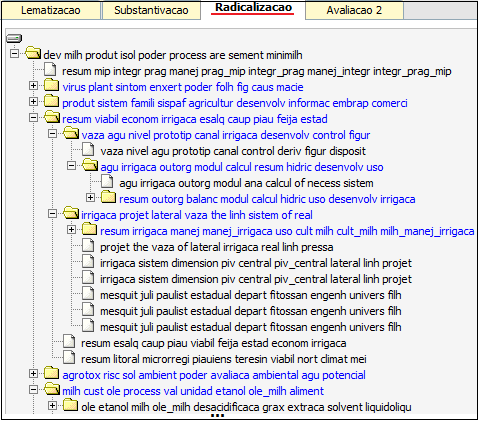
\includegraphics[scale=0.6]{figuras/taxonomia_radic.png}
\caption{Ramos selecionados para avalia��o da t�cnica de radicaliza��o}
\label{fig:taxonomia_radic}
\end{figure}

\begin{figure}
\centering
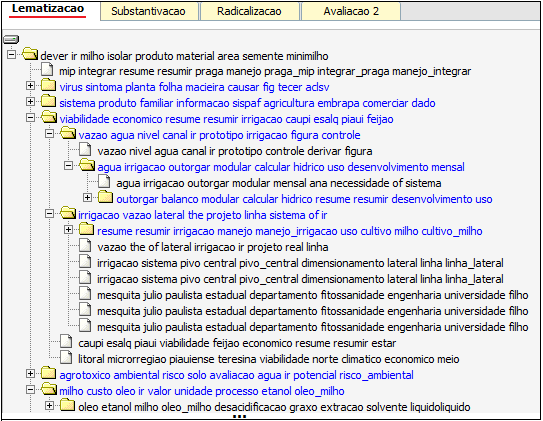
\includegraphics[scale=0.8]{figuras/taxonomia_lemat.png}
\caption{Ramos selecionados para avalia��o da t�cnica de lematiza��o}
\label{fig:taxonomia_lemat}
\end{figure}

\begin{figure}
\centering
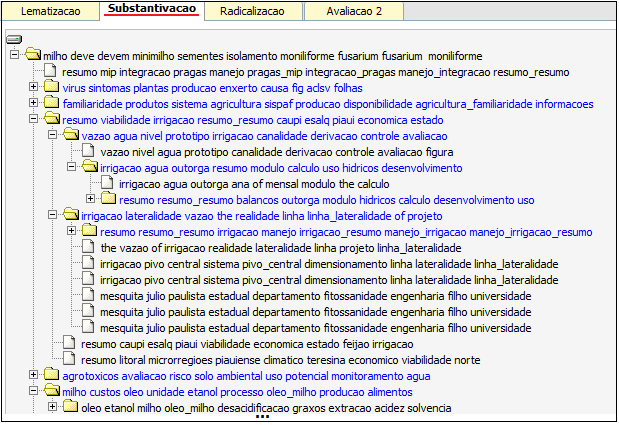
\includegraphics[width=12cm,height=7.7cm]{figuras/taxonomia_subst.png}
\caption{Ramos selecionados para avalia��o da t�cnica de substantiva��o}
\label{fig:taxonomia_subst}
\end{figure}

% Os especialistas foram: Andr� M., Bruno Nogueira, D�bora, Everton Cherman, Fabiano Fernandes, Lucia de Castro, Merley, Rafael Rossi, Ricardo Marcacini, Tatiane Nogueira e V�ctor Laguna.
Onze especialistas do dom�nio atribu�ram � cada ramo das taxonomias uma nota - de um (1) a quatro (4) - em rela��o a representatividade dos termos. Esta avalia��o subjetiva foi auxiliada por meio da ferramenta TaxTool, que possibilidade aos especialistas abrir e ler os documentos que os termos devem representar, permitindo, assim,  uma melhor avalia��o.

Para analisar as notas dadas pelos especialistas, foi utilizado um modelo linear generalizado \citep{Searle:1971} da seguinte forma:

\begin{center}
$\widehat{nota} = \widehat{\mu} + \widehat{noh} + \widehat{tecnica} + \widehat{avaliador} + \widehat{\epsilon}$
\end{center}

\noindent no qual, $\widehat{\mu}$ � a m�dia geral das notas atribu�das pelos especialistas. Os efeitos do modelo, que correspondem aos desvios em rela��o � m�dia geral, s�o representados por $\widehat{noh}$, que corresponde ao n� (ramo) da taxonomia que foi avaliado; $\widehat{tecnica}$, que corresponde a t�cnica avaliada; e $\widehat{avaliador}$, que corresponde ao avaliador. Por fim, tem-se o erro aleat�rio ($\widehat{\epsilon}$), sendo que este n�o � explicado pelos efeitos citados.

As compara��es m�ltiplas de m�dias foram realizadas com o uso do teste SNK  \citep{SneCoch:1967}, considerando 95\% de certeza, no qual os grupos de notas foram representados por letras, ou seja, na tabela que segue, letras iguais correspondem a grupos estatisticamente iguais. Na Tabela \ref{tab:agrup_notas} encontram-se os resultados das compara��es das notas das tr�s t�cnicas utilizadas para cada base de textos, bem como os valores do quadrado m�dio do erro aleat�rio (qme) e os graus de liberdade (g.l) de cada base. Para este teste foi utilizado o software livre MODLIN pertencente � Rede de Software Livre para Agropecu�ria\footnote{Rede de Software Livre para Agropecu�ria - http://www.agrolivre.gov.br/} (Software Cient�fico - SOC) da Embrapa.

% nota-se que apesar da expectativa inicial de que a substantiva��o deveria ser melhor classificada, isso n�o ocorreu. A ``radicaliza��o'' foi ligeiramente melhor classificada que as demais, sendo que as duas outras t�cnicas foram consideradas estatisticamente iguais. 

\begin{table}
	\centering
		\begin{tabular}{|c|c|c|c|c|c|c|}
		\hline
			\it \textbf{Bases} & \it \textbf{g.l} & \it \textbf{qme}	& \it \textbf{T�cnicas}	& \it \textbf{\# notas dadas} & \it \textbf{Ramos} & \it \textbf{Grupos} \\
			\hline
			\hline
			\multirow{3}{*}{Milho} & \multirow{3}{*}{307} & \multirow{3}{*}{0.3875}	& Radicaliza��o 		& 110			& 2.754545			& milho\_b \\ \cline{4-7}
															&&	& Substantiva��o 			& 110 									& 3.009091				& milho\_a \\ \cline{4-7}
															&&	& Lematiza��o 				& 109 									& 2.926606				& milho\_a \\ \cline{4-7}
			\hline
			\hline
			\multirow{3}{*}{Cana} 	&	\multirow{3}{*}{290} & \multirow{3}{*}{0.3634}	& Radicaliza��o 		& 104 	& 2.355769 			& cana\_b \\ \cline{4-7}
															&&	& Substantiva��o 			& 104 										& 2.634615 				& cana\_a \\ \cline{4-7}
															&&	& Lematiza��o 				& 104 										& 2.596154 			& cana\_a \\
			\hline
			\hline
			\multirow{3}{*}{Feij�o} &	\multirow{3}{*}{276} & \multirow{3}{*}{0.3837}	& Radicaliza��o 		& 98 		& 2.551020			& feijao\_b \\ \cline{4-7}
															&&  & Substantiva��o 			& 96 											& 2.979167				& feijao\_a \\ \cline{4-7}
															&&	& Lematiza��o 				& 104											& 2.634615 			& feijao\_b \\
			\hline
			\hline
			\multirow{3}{*}{Leite} 	&	\multirow{3}{*}{307} & \multirow{3}{*}{0.3875}	& Radicaliza��o 		& 110		& 2.754545			& leite\_b \\ \cline{4-7}
															&&	& Substantiva��o 			& 110 										& 3.009091			& leite\_a \\ \cline{4-7}
															&&	& Lematiza��o 				& 109											& 2.926606 			& leite\_a \\
			\hline
			\hline
			\multirow{3}{*}{Ma��} 	&	\multirow{3}{*}{291} & \multirow{3}{*}{0.3720}	& Radicaliza��o 		& 105		& 2.409524			& maca\_b \\ \cline{4-7}
															&&	& Substantiva��o			& 105 										& 3.085714			& maca\_a \\ \cline{4-7}
															&&	& Lematiza��o 				& 106											& 3.009434			& maca\_a \\
			\hline
			\hline
			\multirow{3}{*}{Caupi} 	&	\multirow{3}{*}{267} & \multirow{3}{*}{0.3296}	& Radicaliza��o 			& 97	& 2.381443			& caupi\_b \\ \cline{4-7}
															&&	& Substantiva��o 			& 97 											& 2.793814 							& caupi\_a \\ \cline{4-7}
															&&	& Lematiza��o 				& 97 											& 2.752577 							& caupi\_a \\
			\hline
			\hline
			\multirow{3}{*}{Eucalipto} &		\multirow{3}{*}{185} & \multirow{3}{*}{0.4381}	& Radicaliza��o 	& 57	& 2.543860		& eucalipto\_b \\ \cline{4-7}
															&&	& Substantiva��o 			& 57 											& 2.929825				& eucalipto\_a \\ \cline{4-7}
															&&	& Lematiza��o 				& 99 											& 3.141414 				& eucalipto\_a \\
			\hline
			\hline
			\multirow{3}{*}{Caju} &		\multirow{3}{*}{333} & \multirow{3}{*}{0.3837}	& Radicaliza��o 		& 118		& 2.669492				& caju\_c \\ \cline{4-7}
															&&	& Substantiva��o 			& 118											& 3.211864 				& caju\_a \\ \cline{4-7}
															&&	& Lematiza��o 				& 120 										& 3.025000 				& caju\_b \\
			\hline
		\end{tabular}
		\caption{Agrupamento das notas nos ramos} \label{tab:agrup_notas}
\end{table}



\textbf{An�lise e Resultados:} os resultados das compara��es das notas das tr�s t�cnicas utilizadas para cada base de textos mostraram que, para a base do Caju, houve diferen�a estatisticamente significativa para as tr�s t�cnicas, sendo que o uso da t�cnica de substantiva��o gerou termos mais representativos para esta base, seguida da t�cnica de lematiza��o e, por fim, da radicaliza��o. Este fato provavelmente � explicado pelo tamanho da base, pois a base do Caju � a menor de todas, com apenas 40 (quarenta) documentos. Como a quantidade de termos � pequena, tem-se menos chance de serem escolhidos termos que n�o representam a cole��o, dessa forma, os termos extra�dos com o uso das tr�s t�cnicas tendem a ser mais semelhantes (exceto pela forma de simplifica��o). Isso pode fazer com que os especialistas elejam as t�cnicas cujos termos estejam mais compreens�veis.

J� para a base do Feij�o, o uso da t�cnica de substantiva��o obteve termos mais representativos do que as t�cnicas de lematiza��o e radicaliza��o. Para as demais bases, houve diferen�a estatisticamente significativa positiva para as t�cnicas de substantiva��o e lematiza��o em rela��o � radicaliza��o.

Esta avalia��o mostrou que, segundo os especialistas, exceto para as bases do Feij�o e Caju, obt�m-se termos mais representativos quando utilizada a t�cnica de lematiza��o ou substantiva��o.



%---------------------- Avalia��o 5
\subsection{Avalia��o 5 - Compreensibilidade dos Termos Extra�dos}

\textbf{Objetivo:} avaliar a compreensibilidade dos termos extra�dos utilizando as diferentes t�cnicas de simplifica��o dos termos, bem como analisar os impactos que as diferentes formas de extra��o de termos causaram nos especialistas.

\textbf{Hip�teses:}
\begin{enumerate}
	\item com esta avalia��o ser� poss�vel eleger uma ou mais t�cnica que melhor se aplica ao dom�nio em quest�o, segundo a avalia��o subjetiva dos especialistas;
	\item a extra��o de termos utilizando diferentes t�cnicas, gerar� impactos diferentes nos especialistas;
	\item a t�cnica de radicaliza��o, provavelmente, ser� eleita como a que gera termos menos compreens�veis por ser a mais agressiva em sua aplica��o.%, por�m o custo computacional desta t�cnica em rela��o a radicaliza��o provavelmente ser� maior. Enquanto a lematiza��o equilibrar� estes dois par�metros (custo computacional e compreensibilidade).
\end{enumerate}

\textbf{Descri��o:} a compreensibilidade dos termos extra�dos foi avaliada subjetivamente pelos especialistas do dom�nio, sendo feita separadamente para cada base de textos, conforme mostrado anteriormente na Figura \ref{fig:notasNoh}. Para isso, os especialistas elegeram uma ou mais t�cnicas que consideraram gerar termos mais compreens�veis para a base de textos analisada, isto �, qual (ou quais) t�cnica obteve termos mais f�ceis de serem entendidos pelos especialistas (neste caso, os especialistas s�o os usu�rios finais dos termos). Ressalta-se que, os termos foram avaliados n�o levando em considera��o as taxonomias, sendo que estas foram utilizadas somente para facilitar � avalia��o.

\textbf{An�lise e Resultados:} o resultado desta avalia��o � mostrado na Figura \ref{fig:compreensibilidade}. Pode-se observar que a t�cnica de substantiva��o foi eleita como a que gera termos bem mais compreens�veis do dom�nio de agroneg�cio se comparada com as outras duas t�cnicas. Sendo, portanto, a mais indicada para ser utilizada neste dom�nio quando necessita-se de compreensibilidade nos resultados. Enquanto a t�cnica de radicaliza��o foi eleita como a que gera termos menos compreens�veis, por ser a mais agressiva em sua aplica��o.

\begin{figure}[h]
\centering
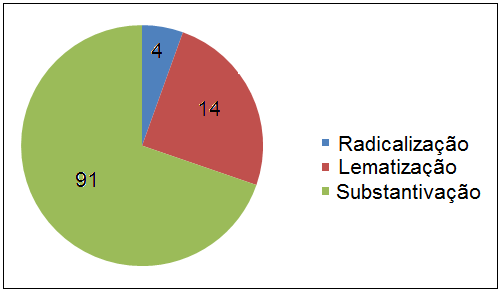
\includegraphics[scale=0.75]{figuras/compreensibilidade.png}
\caption{Avalia��o subjetiva quanto a compreensibilidade dos termos obtidos utilizando as t�cnicas}
\label{fig:compreensibilidade}
\end{figure}

Provavelmente o impacto causado nos especialistas em rela��o � compreensibilidade dos termos, afetou tamb�m a avalia��o subjetiva dos termos quanto �s suas representatividades. Uma poss�vel explica��o seria que, como em alguns casos, determinados termos foram obtidos de uma forma mais f�cil de serem entendidos (menos simplificados) e outros menos f�cil de serem entendidos, mesmo os dois termos estarem se referindo ao mesmo tema, os termos mais compreens�veis podem ser entendidos mais facilmente e, portanto, serem eleitos como mais representativos.


%---------------------- Avalia��o 6
\subsection{Avalia��o 6 - Prefer�ncia dos Especialistas}

\textbf{Objetivo:} apontar, para todas as bases de textos, qual a prefer�ncia geral subjetiva dos especialistas em rela��o �s t�cnicas de simplifica��o de termos, isto �, qual t�cnica os especialistas consideraram melhor para ser utilizada neste dom�nio.

\textbf{Hip�tese:} as t�cnicas de substantiva��o e lematiza��o ser�o eleitas pelos especialistas por gerarem, possivelmente, termos mais compreens�veis do que a t�cnica de radicaliza��o.

\textbf{Descri��o:} os especialistas do dom�nio indicaram suas prefer�ncias gerais por alguma das t�cnicas utilizadas elegendo, para cada base de textos, a t�cnica que consideraram mais adequada para a base, conforme mostrado anteriormente no item ``B'' da Figura \ref{fig:notasNoh}.

\textbf{An�lise e Resultados:} como todas as bases de textos pertencem a um subdom�nio do dom�nio de agroneg�cio, estas prefer�ncias foram consideradas como prefer�ncia geral do dom�nio, sendo que o resultado pode ser observado na Figura \ref{fig:preferencia}.

\begin{figure}[h]
\centering
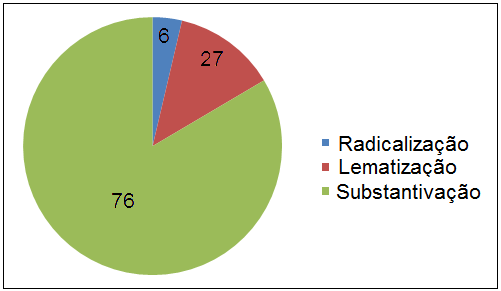
\includegraphics[scale=0.75]{figuras/preferencia.png}
\caption{Avalia��o subjetiva quanto a t�cnica de prefer�ncia dos especialistas}
\label{fig:preferencia}
\end{figure}

Observa-se que a t�cnica de substantiva��o, assim como na avalia��o anterior, foi eleita como a t�cnica que os especialistas preferem para ser utilizada neste dom�nio, seguida da t�cnica de lematiza��o e, depois, da radicaliza��o. Tal escolha tamb�m � devido a compreensibilidade dos termos extra�dos por esta t�cnica, pois esta caracter�stica atrai o usu�rio humano.


%---------------------- Avalia��o 7
\subsection{Avalia��o 7 - Complexidades dos Algoritmos das T�cnicas de Simplifica��o de Termos}

\textbf{Objetivo:} analisar as complexidades dos algoritmos utilizados para a aplica��o das t�cnicas de simplifica��o de termos.

\textbf{Hip�tese:} com a an�lise das complexidades de cada t�cnica � poss�vel escolher qual t�cnica utilizar para auxiliar a extra��o de termos.

\textbf{Descri��o:} foram analisadas as complexidades, no pior caso, dos algoritmos de radicaliza��o, lematiza��o e substantiva��o, considerando somente os passos para a simplifica��o dos termos de cada t�cnica. A descri��o dos algoritmos e de suas complexidades � apresentada a seguir.

Para o algoritmo de radicaliza��o voltado � L�ngua Portuguesa, \citet{pretext2:2008} criaram uma estrutura de dados para armazenar as palavras do documento e cada palavra desse documento � submetida ao processo de radicaliza��o. Conforme pode ser observado no Algoritmo \ref{ALG:radic}, a complexidade do algoritmo de radicaliza��o para cada documento, no pior caso, � $O(|P|)$, sendo $|P|$ a quantidade de palavras do documento.

\begin{algorithm}[h!]
\floatname{algorithm}{Algoritmo}	
	\caption{Radicaliza��o}
	\label{ALG:radic}
	\algsetup{indent=2em}
	\begin{algorithmic}[1]
	\REQUIRE documento original
	\ENSURE documento com palavras radicalizadas
	
		\FORALL {palavras do documento}			
			\IF {palavra � um verbo irregular} %irregPt: no pior caso, faz 986 compara��es.
				\STATE retornar o infinitivo do verbo
			\ELSE
				\IF {tamanho da palavra � menor ou igual a tr�s} %length($word): faz 1 compara��o.
					\STATE retornar a pr�pria palavra
				\ELSE
					\STATE remover os pronomes obl�quos e o plural da palavra %basicStemPt: faz 4 compara��es.
					\STATE remover os sufixos da palavra %stemmerPt: no pior caso, faz 11 compara��es.
					\IF {palavra n�o foi reduzida}
						\IF {palavra � um verbo} %verboPt: no pior caso, faz 3 compara��es.
							\STATE remover sufixos do verbo
						\ENDIF
					\ENDIF
				\ENDIF
			\ENDIF
		\ENDFOR
		
	\end{algorithmic}
\end{algorithm}

%    # Caso seja um verbo irregular, retorna o seu infinitivo
%    $stem = $self->irregPt($word);
%    
%    if ($stem) {
%        return $stem;
%    }
%
%    if (length($word) <= 3) {
%        # Palavras muito pequenas retornam sem stem
%        return $word;
%    } else {
%        # Chama subrotina pra transformar a palavra
%        # em seu stem em Portugues
%        $word = $self->basicStemPt($word);
%        $stem = $self->stemmerPt($word);
%
%        # Se a palavra n�o tem stem, checar se � um verbo
%        if ($word eq $stem) {
%            $stem = $self->verboPt($word);
%        }
%
%        return $stem;
%    }
%}

%%Lematizador de Nunes:
%A complexidade do algoritmo de lematiza��o, como pode ser observados no Algoritmo XX, � constante ($O(1)$), se considerado que o acesso a tabela \textit{hash} tamb�m � constante. Este Hash � gerado, em um processo pr�vio a este algoritmo, a partir de uma base de palavras can�nicas pr�pria do Lematizador de Nunes.
%st = palavra
%se existir palavra no HashDeLema entao
%	MainForm.Table1.FindKey = hashDeLema -> atribui-se a forma can�nica da palavra a vari�vel lema
%else atribui-se a palavra original a vari�vel lema
%
%function lema(st: string): string;
%begin
%        st:=minuscula(st);
%        if (MainForm.Table1.FindKey([st]))
%          then lema:=MainForm.Table1.FieldByName('Can�nica').Value
%          else lema:=st;
%end;

O lematizador utilizado neste trabalho faz uso da base de palavras can�nicas do Lematizador de Nunes \citep{Nunes:1996}. Conforme descrito no Algoritmo \ref{ALG:lemat}, cada palavra presente no documento � substitu�da por seu respectivo lema buscado na base de palavras. Para isso, foi criada uma estrutura \textit{hash} para armazenar os lemas da base, na qual as buscas s�o feitas a partir das palavras originais do documento e s�o retornados seus respectivos lemas encontrados. Considerando que a complexidade de busca da estrutura \textit{hash} � $O(1)$ devido a sua caracter�stica, a complexidade, para cada documento, do algoritmo de lematiza��o desenvolvido neste trabalho � $O(|P|)$, sendo $|P|$ a quantidade de palavras do documento.

%Lematizador adaptado de Nunes:
\begin{algorithm}[h!]
\floatname{algorithm}{Algoritmo}	
	\caption{Lematiza��o}
	\label{ALG:lemat}
	\algsetup{indent=2em}
	\begin{algorithmic}[1]
	\REQUIRE documento original
	\ENSURE documento com palavras lematizadas
	
		\FORALL {palavras do documento}
			\IF {se palavra do documento existe na lista de lemas}		
				\STATE retornar o lema encontrado da palavra
			\ELSE
				\STATE retornar a palavra do documento
			\ENDIF
		\ENDFOR
		
	\end{algorithmic}
\end{algorithm}

		
%		public static void trocar_palavra (File caminhoorigem, File caminhodestino) {
%		try {
%			BufferedReader in = new BufferedReader(new FileReader(caminhoorigem));
%			FileWriter writer = new FileWriter(caminhodestino, true);
%			PrintWriter saida = new PrintWriter(writer, true);
%
%			String palavra_texto = null,
%			palavra_trocada = null,
%			line = in.readLine();
%
%			//while: O(n) sendo n o numero de tokens do arquivo
%			while (line != null) {
%				StringTokenizer tk = new StringTokenizer(line);
%				while (tk.hasMoreTokens()) {
%					palavra_trocada = null;
%					palavra_texto = tk.nextToken();
%
%					palavra_trocada = procuraPalavraTrocada(palavra_texto);					
%
%					if (palavra_trocada == null)
%						saida.print(palavra_texto + " ");
%					else
%						saida.print(palavra_trocada + " ");
%				}
%				line = in.readLine();
%				saida.println();
%			}
%			saida.flush();
%			saida.close();
%			writer.close();
%			in.close();
%
%		} catch (Exception e) {
%			e.printStackTrace();
%		}
%	}
%
%
%	private static String procuraPalavraTrocada(String palavra){
%
%		int posicaoHash = posicaoHash(palavra);
%		String palavraTratada = tratamento(palavra);
%		String palavraTrocada = null;
%		boolean found = false;
%		for(int i = 0; i < tabelaHash.get(posicaoHash).size() && !found; i++){
%			if (tratamento(tabelaHash.get(posicaoHash).get(i).palavra).equals(palavraTratada)){
%				palavraTrocada = tabelaHash.get(posicaoHash).get(i).lema;
%				found = true;
%			}
%		}
%		return palavraTrocada;
%
%	}


Segundo \citet{Gonzalez:2005}, a complexidade do algoritmo de substantiva��o para cada documento, descrito no Algoritmo \ref{ALG:lemat}, � $O(|P|)$, considerando que as �rvores utilizadas no algoritmo est�o parcialmente balanceadas e que o n�mero de adjetivos, adv�rbios, verbos ou substantivos �, no m�ximo, igual a $|P|$, sendo sendo $|P|$ a quantidade de palavras do documento.

\begin{algorithm}[h!]
\floatname{algorithm}{Algoritmo}	
	\caption{Substantiva��o \citep{Gonzalez:2005}}
	\label{ALG:subst}
	\algsetup{indent=2em}
	\begin{algorithmic}[1]
	\REQUIRE documento original
	\ENSURE documento com palavras substantivadas
	
	\FORALL {p $\epsilon$ P = {palavras do documento}}			
		\STATE verificar etiqueta morfol�gica de p
		\IF {p � adv�rbio} 
		        \STATE transformar em adjetivo correspondente
		\ENDIF
		\IF {p � adjetivo ou verbo} 
	        	\STATE pesquisar em aut�mato de exce��es implementado em �rvore tern�ria de pesquisa com $N_E$ nodos
	        	\IF {pesquisa tem sucesso}
	        		\STATE derivar substantivos de p
			\ELSE
				\STATE pesquisar p em aut�mato de adjetivos ou de verbos implementado em �rvore tern�ria de pesquisa com $N_A$ (para adjetivos) ou $N_V$ (para verbos) nodos
			 	\IF {pesquisa tem sucesso}
	      				\STATE derivar substantivos de p
	      			\ELSE
	      				\STATE n�o h� nominaliza��o (substantiva��o) para p
	        		\ENDIF
			\ENDIF
		\ELSE
			\IF {p � substantivo}
				\STATE pesquisar em aut�mato de sin�nimos implementado em �rvore tern�ria de pesquisa com $N_S$ nodos
				\IF {pesquisa tem sucesso}
					\STATE derivar sin�nimo de p
				\ELSE
					\STATE n�o h� sin�nimo de p
				\ENDIF
			\ENDIF
		\ENDIF
	\ENDFOR
	\end{algorithmic}
\end{algorithm}

Logo, a complexidade dos algoritmos de radicaliza��o, lematiza��o e substantiva��o, para cada documento, pertence � classe linear $O(|P|)$.

\textbf{An�lise e Resultados:} ao contr�rio da hip�tese apresentada nesta avalia��o, as complexidades dos algoritmos utilizados para a aplica��o de cada t�cnica n�o s�o um fator determinante na escolha de uma das t�cnicas para auxiliar a extra��o de termos, j� que os tr�s pertencem � classe linear. Por�m, deve-se levar em considera��o que o algoritmo de substantiva��o necessita de que as palavras do documento j� estejam etiquetadas morfologicamente. Al�m disso, neste trabalho, ap�s a obten��o dos substantivos por este algoritmo, � necess�rio escolher qual substantivo ser� considerado (substantivo abstrato ou concreto), conforme explicado anteriormente na Se��o \ref{extracao} do Cap�tulo ~\ref{abordExtracao}. Estes detalhes podem aumentar o custo computacional da aplica��o da t�cnica de substantiva��o em rela��o as outras duas t�cnicas.

%Utilizando os termos gerados no experimento 1, foram calculados os tempos em que cada t�cnica utiliza para simplificar os termos de cada base de textos, conforme mostrado na Tabela~\ref{tab:tempo_tecnicas}.
%
%\begin{table}[!ht]
%\centering \scriptsize
%\begin{tabular}{|c|c|c|c|c|c|c|c|c|}
%\hline
%\multirow{2}{*}{\it \textbf{Tempo por t�cnica}} & \multicolumn{8}{|c|}{\it \textbf{Base de Textos (Produto)}}\\ \cline{2-9}
%& Milho & Cana & Feij�o & Leite & Ma�� & Caupi & Eucalipto & Caju\\ \hline \hline
%Radicaliza��o & & & & & & & & \\ \hline
%Lematiza��o &810.221&1.059.655&613.138 & 201.806 & 440.089 & 952.364 & 67.128 & 50.835 \\ \hline
%Substantiva��o & 63.569 & 51.965 & 43.906 & 39.593 & 29.559 & 29.405 & 12.186 & 5.073\\ \hline
%\end{tabular}
%\caption{Tempo da aplica��o de cada t�cnica (em milisegundos)} \label{tab:tempo_tecnicas}
%\end{table}

%\textbf{An�lise e Resultados:}
%Quanto ao tempo de simplifica��o de termos, observa-se que, geralmente, a t�cnica de radicaliza��o foi executada em um tempo inferior as outras t�cnicas, seguida da substantiva��o e depois da lematiza��o. Deve-se ressaltar que os autores destas t�cnicas visavam seus pr�prios objetivos em suas implementa��es, mas tamb�m deve-se lembrar que o tempo de execu��o de alguma tarefa pode influenciar na escolha do uso de alguma das t�cnicas quando se necessita de um desempenho melhor ou quando a base de textos possui um tamanho muito elevado.


%%%%%%%%%%%%%%%%%%%%%%%%%%%%%%%%%%%%%%%%%%%%%%%%%%%%%%%%%%%%%%%%%
%   Considera��es Finais
%%%%%%%%%%%%%%%%%%%%%%%%%%%%%%%%%%%%%%%%%%%%%%%%%%%%%%%%%%%%%%%%%
\newpage
\section{Considera��es Finais}
Neste cap�tulo foram descritas as avalia��es subjetivas e objetivas adotadas para avaliar os termos extra�dos deste trabalho. As avalia��es subjetivas tendem a ser custosas, pois demandam mais tempo para sua execu��o, e al�m de necessitar da disponibilidade de especialistas do dom�nio pode ser influenciada por prefer�ncias pessoais dos mesmos. Mesmo com estas dificuldades, a presen�a dos especialistas � vantajosa, j� que os mesmos, neste caso, s�o os usu�rios finais dos termos. Adicionalmente, estas avalia��es subjetivas s�o necess�rias para avaliar a compreensibilidade dos termos obtidos.

Neste cap�tulo tamb�m foi realizada a avalia��o experimental seguindo os passos da metodologia de extra��o de termos. Com isso foi poss�vel observar que, conforme mostrado na Tabela \ref{tab:quant_termos}, o uso da metodologia contribui consideravelmente para a diminui��o da quantidade de termos extra�dos, pois al�m de simplificar os termos com tr�s diferentes t�cnicas, faz uso de m�todos estat�sticos para remover as palavras que n�o s�o bons candidatos a termos.

Mesmo assim, foram mantidos alguns termos que deveriam ter sido exclu�dos, como termos que possuem algum verbo que n�o contribui para a obten��o de termos representativos da cole��o (como \textit{manejo\_integrar}), ou ainda bigramas e trigramas compostos por palavra repetidas (como \textit{resumo\_resumo}). Estes termos podem ser vistos, respectivamente, nas Figuras \ref{fig:taxonomia_lemat} e \ref{fig:taxonomia_subst} deste cap�tulo. Uma poss�vel solu��o para este problema, seria incrementar a metodologia com t�cnicas ling��sticas capazes de identificar se a presen�a de determinados verbos � relevante ou n�o para o termo.

Tamb�m foram descritos experimento e avalia��es desses experimentos, juntamente com os resultados e an�lises dos mesmos, sobre a representatividade dos termos extra�dos sob a vis�o subjetiva dos especialistas e sob uma medida objetiva, a CTW (\textit{Context Term Weight}). Bem como, segundo os especialistas, sobre a compreensibilidade dos termos extra�dos com o uso de cada t�cnica e a que os especialistas sugerem para ser utilizada no dom�nio de agroneg�cio.
 
No cap�tulo a seguir, s�o apresentadas as conclus�es e as principais contribui��es alcan�adas com o desenvolvimento deste trabalho, bem como sugest�es de trabalhos futuros.


\chapter{Conclus�es} \label{acabou}


\section{Contribui��es}

Este trabalho teve por objetivo identificar um processo para desenvolvimento de projetos de pesquisa envolvendo software, tendo em vista o aux�lio � evolu��o desses projetos. Uma das principais dificuldades relatadas na literatura est� relacionada � car�ncia de documenta��o em um ambiente em que h� alta rotatividade dos membros que participam das equipes. Esta foi uma importante motiva��o para que o processo de documenta��o fosse investigado de forma mais detalhada, considerando-se a abordagem de {\it design rationale}. 

As principais contribui��es deste trabalho e as experi�ncias relacionadas podem ser resumidas conforme apresentadas a seguir:

\begin{enumerate}

\item Identifica��o de um processo para desenvolvimento de projetos de pesquisa, utilizando-se uma abordagem sistem�tica proposta na literatura. O uso da abordagem proposta por Humphrey para a defini��o do processo foi relevante, pois indicou etapas fundamentais, como a identifica��o de requisitos para o processo, que guiaram efetivamente o desenvolvimento da proposta. Al�m disso, acredita-se que a documenta��o gerada com o cumprimento de cada etapa contribuir� para a evolu��o e melhoria da proposta.    

\item Identifica��o de um modelo de {\it design rationale} para projetos de pesquisa, considerando-se caracter�sticas do dom�nio. Estudos de caso foram realizados no decorrer do trabalho e os resultados obtidos, as experi�ncias realizadas e as li��es aprendidas fundamentaram a elabora��o da proposta. Al�m disso, o fato de ter sido cumprido um ciclo de desenvolvimento para a obten��o do modelo, incluindo identifica��o de requisitos, projeto, implementa��o e experimenta��o, foi fundamental no sentido de possibilitar o refinamento gradual da proposta.   

\end{enumerate}    

Nota-se que as contribui��es est�o inseridas em um contexto de pesquisa que est� sendo valorizado atualmente. H� diversos incentivos para que projetos de pesquisa sejam desenvolvidos de forma colaborativa, envolvendo pesquisadores de diferentes �reas de conhecimento, tendo em vista aos avan�os cient�ficos e tecnol�gicos. Como resultado, a comunidade cient�fica est� come�ando a propor discuss�es de amplo alcance em torno do tema de \textbf{processos} para o desenvolvimento de projetos de pesquisa. Um exemplo disso � a realiza��o do {\it First International Workshop on Improving Research Productivity in Computing}\footnote{http://www.iaria.org/conferences2007/IRP.html}, a ser realizado em agosto de 2007 na Fran�a, que tem por objetivo discutir {\it como} os projetos de pesquisa est�o sendo desenvolvidos e quais s�o as alternativas para melhorar os processos utilizados.   

\section{Limita��es} \label{limita}

Algumas limita��es deste trabalho foram:

\begin{itemize}

\item Alguns requisitos identificados pelos usu�rios, por exemplo, gerenciamento de conhecimentos, n�o foram cobertos pois optou-se por propor uma solu��o inicial que dever� ser avaliada, melhorada e estendida de forma incremental; 

\item A descri��o das atividades, tarefas e artefatos do processo � simplificada e oferece apenas uma vis�o geral do trabalho que precisa ser realizado;

\item A abordagem iterativa, mencionada como um requisito de um processo para desenvolvimento de projetos de pesquisa em software, n�o foi experimentada;

\item A avalia��o e a valida��o do processo proposto foram pouco enfatizadas, sendo necess�ria, principalmente, a realiza��o de experimentos reais no contexto de desenvolvimento de projetos de pesquisa colaborativos e distribu�dos;

\item A proposta envolvendo {\it design rationale} n�o foi analisada em rela��o �s atividades de captura e recupera��o das informa��es. � importante averiguar o quanto essas atividades podem ser cumpridas satisfatoriamente quando o modelo � utilizado.  

\end{itemize}

\section{Trabalhos futuros}

Al�m das propostas de trabalhos futuros indicadas nos cap�tulos anteriores, podem ser destacadas:  

\begin{itemize}

\item Definir formalmente a sint�tica e a sem�ntica do processo; 

\item Desenvolver um ambiente que auxilie a execu��o das atividades propostas e o armazenamento e a recupera��o de informa��es relacionadas aos projetos de pesquisa. Uma possibilidade � a investiga��o da adequa��o de ambientes que j� foram desenvolvidos, por exemplo, a esta��o TABA \citep{roch05} nesse escopo. Certamente este ser� um facilitador para o cumprimento das etapas 7 e 8 propostas por Humphrey, que se referem � valida��o e melhoria do processo; 

\item Investigar se os modelos de avalia��o de processos de software atuais s�o aplic�veis ao contexto de desenvolvimento de projetos de pesquisa. Caso n�o sejam, investigar quais elementos devem compor tais modelos. Observa-se que alguns pesquisadores est�o come�ando a se interessar em avaliar os processos que cumprem nos laborat�rios de pesquisa, com o objetivo de atrair e viabilizar novas parcerias com outros centros de pesquisa e com o setor industrial. Um modelo de avalia��o, portanto, complementa a proposta apresentada neste trabalho;

\item Investigar as principais caracter�sticas que definem um ambiente {\it collaboratory} e determinar o quanto a proposta apresentada est� alinhada aos seus objetivos, propondo e realizando as modifica��es necess�rias;

\item Dar continuidade �s investiga��es relacionadas a um modelo de maturidade para o desenvolvimento de projetos de pesquisa envolvendo software, observando a viabilidade em tratar a especializa��o dos n�veis 4 e 5 do CMMI para esse contexto;

\item Realizar experimentos com o modelo de {\it design rationale} em um ambiente de desenvolvimento de pesquisas;

\item Investigar a possibilidade de aplica��o da abordagem de {\it design rationale} como uma forma de capturar o conhecimento dos pesquisadores em rela��o a cada um dos processos apresentados na Figura \ref{fig1};

\item Cobrir os requisitos de {\it evolu��o de design rationale} e {\it informa��es de contexto} do modelo de representa��o, discutidos na Se��o \ref{mod_re}.
  
\end{itemize}


\section{Produ��o cient�fica}

A seguir est�o as refer�ncias das publica��es decorrentes dos estudos realizados e dos resultados obtidos durante o desenvolvimento da pesquisa descrita nesta tese.  

\subsubsection{Artigos completos em peri�dicos}

\begin{enumerate}

\item Paiva, D. M. B.; Freire, A. P.; Lucr�dio, D.; Braga, R. T. V.; Fortes, R. P. M. ``Reinforcing Design Rationale in Software Projects Developed in Academic Environment.'' \textit{International Transactions on Systems Science and Applications}, 2007. Aceito para publica��o.

\item Freire, A. P.; Paiva, D. M. B.; Fortes, R. P. M. ``Implanta��o de Gest�o Descentralizada de Recursos Acad�micos - um estudo de caso.'' \textit{Revista Brasileira de Inform�tica na Educa��o}, v. 12, n. 2, p. 78-85, 2004. 

\end{enumerate}

\subsubsection{Artigos completos em congressos}

\begin{enumerate}

\item Paiva, D. M. B.; Turine, M. A. S.; Fortes, R. P. M. ``Processo de Software Livre em Ambiente Acad�mico: Experi�ncias e Li��es Aprendidas.'' \textit{Proceedings}. In: CLEI 2006 - XXXII Conferencia Latinoamericana de Inform�tica, Chile, 2006.  

\item Paiva, D. M. B.; Lucr�dio, D.; Fortes, R. P. M. ``MVCASE - Incluindo Design Rationale para Aux�lio � Modelagem em Projetos de Pesquisa.'' \textit{Anais.} In: XVIII Sess�o de Ferramentas do XX Simp�sio Brasileiro de Engenharia de Software,  Florian�polis-SC, p. 73-78, 2006.  

\item Paiva, D. M. B.; Fortes, R. P. M. ``Design Rationale in Software Engineering: A Case Study.'' \textit{Proceedings.} In: Seventeenth International Conference on Software Engineering \& Knowledge Engineering (SEKE), Taiwan, p. 342-348, 2005.

\item Paiva, D. M. B.; Manduca, A. M.; Silva, M. A. G.; Quemello, L. J.; Braga, R. T. V.; Fortes, R. P. M.  ``Refor�ando a Comunica��o com Uso de uma Ferramenta de Software Livre em Ensino de Engenharia de Software.'' \textit{Anais.} In: XIII Workshop sobre Educa��o em Computa��o (WEI 2005), XXV Congresso da Sociedade Brasileira de Computa��o (SBC 2005), S�o Leopoldo-RS, 2005. 

\item Paiva, D. M. B.; Fortes, R. P. M. ``Model for Academic Software Development Including Design Rationale Elements.'' \textit{Proceedings.} In: I IFIP Academy on the State of Software Theory and Practice - PhD Colloquium, Porto Alegre-RS, 2005.  

\item Cagnin, M. I.; Paiva, D. M. B.; Maldonado, J. C.; Penteado, R. D.; Fortes, R. P. M.; Germano, R. S. ``From Design Rationale to Reengineering Rationale: Lessons Learned in a Maintenance Pilot Case Study.'' \textit{Proceedings.} In: 4� Jornadas Iberoamericanas de Ingenier�a del Software e Ingenier�a del Conocimiento, Espanha, p. 231-243, 2004.  

\item Paiva, D. M. B.; Freire, A. P.; Sanches, R.; Fortes, R. P. M. ``Definindo, Implantando e Melhorando Processos de Software em Ambiente Acad�mico.'' \textit{Anais.} In: VI Simp�sio Internacional de Melhoria de Processo de Software (SIMPROS), S�o Paulo-SP, p. 71-82, 2004.  

\item Paiva, D. M. B.; Sanches, R.; Fortes, R. P. M. ``Melhoria de Processo de Software no Contexto do Desenvolvimento Acad�mico de uma Agenda na {\it Web}.'' \textit{Anais.}  In: 14o Congresso Internacional de Tecnologia de Software (CITS 2003), Curitiba-PR, p. 56-68, 2003. 

\item Francisco, S. D.; Izeki, C. A.; Paiva, D. M. B.; Fortes, R. P. M. ``Um Sistema de Apoio � Utiliza��o de Design Rationale de Artefatos de Software.'' \textit{Proceedings.} In: CLEI 2003 - XXIX Conferencia Lationoamericana de Inform�tica, Bol�via, 2003.

\item Francisco, S. D.; Izeki, C. A.; Paiva, D. M. B.; Fortes, R. P. M. ``DocRationale: Um Aux�lio a Design Rationale na Documenta��o de Software.'' \textit{Anais.} In: X Sess�o de Ferramentas, XVII Simp�sio Brasileiro de Engenharia de Software (SBES2003), Manaus-AM, p. 61-66, 2003.  

\end{enumerate}

\subsubsection{Resumos}

\begin{enumerate}

\item Paiva, D. M. B.; Freire, A. P.; Fortes, R. P. M. ``Design Rationale in Academic Software Development: Requirements for a Representation Model.'' \textit{Proceedings.} In: Eighteenth International Conference on Software Engineering \& Knowledge Engineering (SEKE), USA, p. 469-472, 2006.

\item Lara, S. M.; Freire, A. P.; Paiva, D. M. B.; Fortes, R. P. M. ``Registering Design Rationale in Collaborative Software Projects: a Case Study.'' \textit{Proceedings.} In: 4th International Information and Telecommunication Technologies Symposium (I2TS), Florian�polis-SC, p. 163-164, 2005.

\item Freire, A. P.; Paiva, D. M. B.; Fortes, R. P. M. ``Manuten��o de Aplica��es {\it Web} Utilizando Separa��o de Interesses: Um Estudo de Caso.'' \textit{Proceedings.} In: 4th International Information and Telecommunication Technologies Symposium (I2TS), Florian�polis-SC, 2005.  

\item Fortes, R. P. M.; Freire, A. P.; Vieira, V. H.; Paiva, D. M. B. ``An Academic Web-Based Agenda and its Engineering Process.'' \textit{Proceedings.} In: VII Workshop Iberoamericano de Ingenier�a de Requisitos Y Desarrollo de Ambientes de Software, Peru, p. 151-156, 2004. 

\end{enumerate}

\subsubsection{Relat�rio t�cnico}

\begin{enumerate}

\item Paiva, D. M. B.; Freire, A. P.; Fortes, R. P. M. ``Web Engineering Process - a Case Study from Academic Development.'' Relat�rio T�cnico do ICMC-USP, n. 79, 2004. 


\end{enumerate}

\subsubsection{Outras publica��es} 

\begin{enumerate}

\item Freire, A. P.; Paiva, D. M. B.; Turine, M. A. S.; Fortes, R. P. M. ``Using Screen Readers to Reinforce Web Accessibility Education.'' \textit{Proceedings.} To Appear in: 12th Annual Conference on Innovation and Technology in Computer Science Education, Esc�cia, 2007. 

\item Martins Netto, O. A.; Paiva, D. M. B.; Pimentel, M. G. C. ``Abordagem para Deriva��o de Regras de Usabilidade Especializadas em Contextos de Aplica��o Espec�ficos.'' \textit{Proceedings.} In: CLEI 2004 - XXX Conferencia Latinoamericana de Inform�tica, Peru, p. 789-800, 2004. 

\item Fortes, R. P. M.; Silva, E. A.; Paiva, D. M. B. ``Utilizando a Norma ISO/IEC 14598-5 na Avalia��o da Qualidade de Hiperdocumentos {\it Web}.'' \textit{Anais.} In: I Simp�sio Brasileiro de Qualidade de Software (SBQS), Gramado, p. 128-142, 2002. 

\end{enumerate}

\subsubsection{Artigo em avalia��o}

\begin{enumerate}

\item Paiva, D. M. B.; Sanches, R.; Fortes, R. P. M. ``Um Processo para Desenvolvimento de Projetos de Pesquisa Envolvendo Software.'' Submetido ao VI Simp�sio Brasileiro de Qualidade de Software (SBQS), 2007.

\end{enumerate}

%\chapter{Teste}
%\versal{T}este

%\bibliographystyle{apalike} -> aparece n�meros qdo a bibliografia � citada
\bibliographystyle{icmc2} %  -> aparece o nomes dos autores e ano qdo a bibliografia � citada

%%% arquivo .bib
\addcontentsline{toc}{chapter}{Refer�ncias}
\bibliography{root}


%\appendix % Ap�ndices:
%\input{apendice_complexidade}
%\input{apendice_termos}

% Set the ending of a LaTeX document
\end{document}
